\chapter{Traffic analysis using Application Flow Monitoring}\label{chap:traffic-analysis-using-application-flow-monitoring}

\begin{chapintro}

There are many usages for application traffic monitoring. The common goal is to extend the set of collected information elements and thus provide a deeper understanding of network traffic. This chapter shows several use cases for application flow monitoring, that were published in separate papers. The contribution of this chapter is a summary of the contributions of those papers.

As a first example of traffic analysis with the use of application flow monitoring, we show how information from HTTP headers can be used to detect new classes of attacks on the application layer. This is the most common use case for application flow monitoring. 

% Basic flow monitoring usually stops after the first header following the IP layer. However, the IPv6 protocol allows header chains of an arbitrary length. Therefore, we have extended the analysis of IPv6 protocol so that information about multiple chained headers are collected for each flow. An analysis of chained headers is performed and we attempted to interpret their usage. Moreover, we show that these chained headers can be used for attacks and also show, how to detect such attacks using the application flow monitoring. In addition to this work, we also show how IPv6 transition mechanisms can be monitored so that even tunnelled IPv6 traffic can be monitored.

Basic flow monitoring usually stops after the first header following the IP layer. However, many networks and networking protocols utilize encapsulation to traverse over network segments with unsupported equipment or to allow aggregating of traffic into virtual networks. IPv6 transition mechanism are a special class of protocols used to provide IPv6 connectivity over IPv4 networks. Most operating systems provide means to deliver IPv6 connectivity even when native IPv6 is not available. Therefore, we extended the basic flow monitoring with information from the IPv6 transition mechanisms and we report on the IPv6 deployment and the use of the transition mechanisms.

Inserting information to the flow records from external sources is also considered to be a variant of application flow monitoring. We show an example of adding geolocation information both in the flow exporter and collector. We show that both implementations scale very well and that the geolocation data can be used for advanced traffic analysis.

Since most flow monitoring experiments are performed on a live network, it is impossible to exactly replicate the results. We show a method of characterising network traffic so that it is possible to compare multiple network traces and search for similarities. This allows us not only to compare different networks but to quantify changes in network profile in time.

% Martin Husák, Petr Velan, and Jan Vykopal. “Security Monitoring of HTTP Traffic Using Extended Flows”.
% Martin Elich, Petr Velan, Tomáš Jirsík, and Pavel Čeleda. “An Investigation Into Teredo and 6to4 Transition Mechanisms: Traffic Analysis”.
% Pavel Čeleda, Petr Velan, Martin Rábek, Rick Hofstede, and Aiko Pras. “Large-Scale Geolocation for NetFlow”
% Luuk Hendriks, Petr Velan, Ricardo de O. Schmidt, Pieter-Tjerk de Boer, and Aiko Pras. “Threats and Surprises Behind IPv6 Extension Headers”.
% Luuk Hendriks, Petr Velan, Ricardo de O. Schmidt, Pieter-Tjerk de Boer, and Aiko Pras. “Flow-Based Detection of IPv6-specific Network Layer Attacks”
% Petr Velan, Jana Medková, Tomáš Jirsík, and P. Čeleda. “Network Traffic Characterisation Using Flow-Based Statistics”. - needs proper intro in chapintro, or move to next chapter
The papers included in this chapter are~\cite{Husak-2015-Security, Elich-2013-Investigation, Celeda-2013-Large, Velan-2016-Network}. Other papers related to this chapter are~\cite{Hendriks-2017-Flow, Hendriks-2017-Threats}.

The organisation of this chapter is as follows:
\begin{itemize}
  \item Section~\ref{sec:analysis-http-flows} analyses HTTP traffic in a large-scale environment with the use of application flow monitoring. The added value of application flow monitoring is established by detection of several previously undetected attacks.
  \item Section~\ref{sec:analysis-ipv6-transition} reports on IPv6 deployment and the use of transition mechanisms. The basic flow monitoring is extended by the capability of analysing a tunnelled IPv6 traffic.
  \item Section~\ref{sec:analysis-geolocation} shows how flow records can be extended with geolocation information and how this additional information can be employed for network analysis.
  \item Section~\ref{sec:analysis-characterisation} proposes a network traffic characterisation method using flow-based statistics. The characteristics are used to better understand and describe the nature of the traffic and to compare different network traces against each other.
  \item Section~\ref{sec:use-cases-summary} summarizes the chapter.
\end{itemize}

\end{chapintro}

\newpage

\section{Security Monitoring of HTTP Traffic Using Extended Flows}\label{sec:analysis-http-flows}

HTTP is currently the most widely used protocol which takes up a significant portion of network traffic. Due to its popularity, it is beneficial to have a deeper understanding of HTTP network traffic and its content. From a network security perspective, we would like to know who is accessing our network and what the requested resources are. Patterns in network traffic and outstanding numbers of visited hosts and requested resources would help us to distinguish between legitimate and malicious traffic. The most suitable way of gaining an overview of HTTP traffic in a large-scale network is application flow monitoring, as defined in the previous chapter.

We address two problems in this section. The first one is the lack of an overview of network traffic and insufficient security awareness. This applies especially in heterogeneous networks with distributed administration. Many administrators oversee web servers in their administration and may oversee their neighbourhood, but they are not aware of security threats in the rest of the network. The second problem is to find a suitable set of tools to analyse HTTP traffic and distinguish between legitimate and malicious traffic.

To formalize the scope of our work, we pose two research questions which we shall answer:
\begin{itemize}
\item[\emph{(i)}] \emph{What classes of HTTP traffic relevant to security can be observed at network level and what is their impact on attack detection?}
\item[\emph{(ii)}] \emph{What is the added value of application flow monitoring compared to basic flow monitoring from a security point of view?}
\end{itemize}

The first question is focused on common types of HTTP traffic that we can observe in the network. We expect to extend the traditional division of network hosts into clients and servers. We focus on the behaviour of hosts regardless of their client/server role: we are particularly interested in detecting security-related patterns produced by attackers, proxies, and crawlers. We search for implications of the presence of particular traffic patterns. We aim to improve malicious traffic detection, filter out false positives, apply better security policy, and set up trustworthy honeypots.

The second question is focused on evaluating the contribution of application flow monitoring with respect to the detection of malicious behaviour in the network. We focus on the detection of patterns in the network traffic that are hard to observe using basic flow. Application flow would make detecting these events straightforward.

Our work contributes to a better understanding of current security threats. For example, we can detect vulnerability scanners and learn about vulnerability itself at the same time.

The answers to both questions are based on an analysis of real traffic in a campus network. We use network application flow monitoring processing the information from HTTP application layer, which provides HTTP elements to application flow records. Although it is possible to extract some information, such as the Server Name Indication, from the HTTPS protocol, this work focuses on the HTTP protocol only.

We also use auxiliary methods to verify and validate the results, i.e., to confirm the membership of detected IP addresses into the proposed behaviour classes. Legitimate sources of traffic should be identifiable, e.g., Googlebot can be identified by a reverse DNS record of the source IP address~\cite{Google--Verifying}. We check User-Agents in HTTP traffic to differentiate legitimate and illegitimate traffic, e.g., requests with forged User-Agent. Finally, we check the reachability of traffic destination through search engines to see if it is possible to find the resource without accessing it. We follow the principle of ``Google Hacking''~\cite{Billig-2008-Evaluation}, a technique used for finding vulnerabilities on web pages indexed by search engines.

This section is divided into six subsections. Subsection \ref{subsec:httpsecurity-related_work} presents previous work in this field. Measurement tools and environment are described in Subsection \ref{subsec:httpsecurity-measurement}. The results are presented in Subsection \ref{subsec:httpsecurity-results} and discussed in Subsection \ref{subsec:httpsecurity-discussion}. Finally, Subsection \ref{subsec:httpsecurity-conclusion} concludes the section.

\subsection{Related work}\label{subsec:httpsecurity-related_work}

Although research has focused on analysis of HTTP traffic in recent years, there is only a small number of papers relevant to our work. To the best of our knowledge, we are not aware of any paper dealing with HTTP analysis using a flow-based approach. In addition to this, the motivation of the relevant papers is different, typically focusing on efficient traffic management, with only a minor focus on security, specifically attack detection and prevention. One exception is the work by~\citeauthor{Perdisci-2010-Behavioral}~\cite{Perdisci-2010-Behavioral}. They employed network-level behavioural clustering of HTTP requests generated by malware. Their motivation was to provide quality input for algorithms that automatically generate network signatures. The second exception is the work by~\citeauthor{Husak-2014-PhiGARo}~\cite{Husak-2014-PhiGARo} in which they use flow-based HTTP analysis to detect users who contacted malicious websites.

Other related papers dealing with HTTP traffic analysis are listed in this paragraph. \citeauthor{Augustin-2011-Traffic}~\cite{Augustin-2011-Traffic} published a classification of web applications according to three traffic features: intensity (total volume of exchanged traffic), symmetry (ratio between upstream and downstream traffic) and shape (burstiness over time). \citeauthor{Xie-2013-ReSurf}~\cite{Xie-2013-ReSurf} addressed reconstructing web surfing behaviour from network packet traces. \citeauthor{Xu-2014-Toward}~\cite{Xu-2014-Toward} analysed User-Agents strings captured at the edge of a campus network using an extension of UASparser~\cite{Mallat-2017-UASparser}. They identified operating systems, types of devices (mobile, desktop) and applications (browser, crawler, P2P, automated updates and requests). A similar work by~\citeauthor{Jin-2012-Integrated}~\cite{Jin-2012-Integrated} is motivated by efficient traffic management. \citeauthor{Hur-2012-Towards}~\cite{Hur-2012-Towards} proposed a smart phone traffic classification based on grouping User-Agent fields and extracting common strings.

\subsection{Measurement tools and environment}\label{subsec:httpsecurity-measurement}

This section describes the methods and tools used for acquiring the data from our campus network. We shall also provide characteristics of the network, in terms of its size and utilization.

We performed all measurements on the campus network of Masaryk University. The network has more than 40,000 users and 15,000 active IP addresses each day in /16 network segment. The network contains both servers and client stations, including proxy servers and a segment of honeypots. Any incoming traffic to the honeypots is by nature suspicious~\cite{Provos-2007-Virtual}, which helps us to recognize malicious network traffic, e.g., HTTP requests on a honeypot web server. Only moderate filtering rules are applied globally to preserve the network neutrality of the academic environment.

Our primary source of data for network traffic analysis are FlowMon~\cite{FlowmonNetworks--Flowmon} probes located throughout the campus network. These probes use NetFlow and IPFIX protocols to export measured traffic as flow records to central collectors~\cite{Hofstede-2014-Flow}. The collected flows are processed by various anomaly and intrusion detection systems, which report incidents to our CSIRT team. This network-centric approach allows us to monitor a complex network with many servers and services managed by different entities as opposed to host-based approaches such as log analysis. In such a case, it would be very difficult to even obtain system logs from every web server in such a varied environment. The monitored links are mostly 1\,Gb/s and 10\,Gb/s which makes the use of DPI systems impractical, or even impossible in the case of 10\,Gb/s links, due to high processing requirements.

To capture data for this section, we used a probe measuring traffic from a 10\,Gb/s link which connects the campus to the ISP. We deployed measurement of the HTTP traffic on this probe using an application flow exporter. The exporter software supports the extraction of basic elements from HTTP headers, such as host name, document URL (split into hostname and path), User-Agent string, and response code. These elements are then exported using the IPFIX protocol as enterprise elements~\cite{rfc7011}. We used an IPFIXcol~\cite{Velan-2012-Flow} flow collector to receive and store the application flow records.

A basic flow record usually consists of flow keys~\eqref{eq:httpsecurity-flow-key} and of other properties providing detailed information about the flow~\eqref{eq:httpsecurity-flow-additional}. The most common flow keys are L3/L4 protocol numbers, IP addresses, and ports. Additional elements usually contains information from packet headers together with statistical counters, e.g., timestamps, number of packets and bytes, and autonomous system numbers.

\begin{equation} \label{eq:httpsecurity-flow-key}
    \begin{split}
        F_{key} =\ &(L3Proto, srcIP, dstIP, \\
        & L4Proto, srcPort, dstPort)
    \end{split}
\end{equation}

\begin{equation} \label{eq:httpsecurity-flow-additional}
    \begin{split}
        F_{additional} =\ &(timeStart, timeEnd, packets, octets, \\
        & TCPflags, ToS, srcAS, dstAS )
    \end{split}
\end{equation}

A basic flow record is then a concatenation of $F_{key}$ and $F_{additional}$. The HTTP measurement~\cite{Velan-2013-Design} adds information from the HTTP application layer~\eqref{eq:httpsecurity-key-http}. 

\begin{equation} \label{eq:httpsecurity-key-http}
    \begin{split}
        F_{HTTP} =\ &(hostname, path, userAgent, requestMethod, \\
        & responseCode, referrer, contentType )
    \end{split}
\end{equation}

By concatenating a basic flow record with additional application elements an application flow record is created. In this case, it contains HTTP elements~\eqref{eq:httpsecurity-app-flow}.

\begin{equation} \label{eq:httpsecurity-app-flow}
        F_{app} = F_{key} \cdot F_{additional} \cdot F_{HTTP}
\end{equation}

We measured the $F_{app}$ vector in the environment of our campus network for three weeks over the summer break and three weeks in the semester. Thus, we could compare the amount of overall network traffic and suspicious events over two distinct time periods and traffic loads of the network. The amount of the traffic is lower in the summer break, although still comparable to the rest of the year. However, we assume that the amount of malicious traffic is constant over the year and is more apparent in the summer break.

Table~\ref{tab:httpsecurity-data-sets} shows the size of each data set in packets, bytes, and flows. Moreover, it contains the number of HTTP requests observed. Although the number of requests is not high compared to the number of flows, there are at least as many responses, which often carry multimedia content. Therefore, the portion of HTTP traffic in bytes is very significant, despite the lower number of requests.

\begin{table}[ht]
\centering
\begin{tabular}{| c | c | c | c | c |} \hline
Data set &  Flows & Packets & Bytes & HTTP Req.\\ \hline
Summer 2014 & 3.733\,G & 188.953\,G & 198.362\,TB & 0.310\,G \\ \hline
Spring 2015 & 6.680\,G & 552.523\,G & 604.704\,TB & 0.720\,G \\ \hline
\end{tabular}
\caption{Data Sets}
\label{tab:httpsecurity-data-sets}
\end{table}


\subsection{Results}\label{subsec:httpsecurity-results}

Four characteristics of network flows were monitored: source IP address, destination IP address, hostname, and HTTP request. We analysed only HTTP traffic incoming to our network. The destination IP addresses were restricted to the /16 IP range of Masaryk University, while the source IP addresses were restricted to all other IP ranges. In some selected cases, we evaluated also the HTTP requests in opposite direction, i.e., source IP was in our network range and the destination IP was not. We used the hostnames and destination IP addresses interchangeably during the analysis due to a negligible amount of multi-hosting in our network. Overall, we observed HTTP traffic sent to almost 500 web servers, i.e., approximately 3\,\% of all hosts in our network. IPv6 traffic and measurement artifacts were observed in the measurement, but were omitted from the analysis due to their negligible impact on results.

The network traffic was analysed over five-minute and one-day intervals. A five-minute interval is the default granularity of data capture in network flow monitoring, i.e., one output file contains records of five minutes of network traffic. It allowed us to observe local anomalies, not only anomalies in the overall sample traffic. The one-day interval allowed us to compare anomalies over different days and discover repeated events and typical patterns. The one-day time window was chosen as it is long enough to contain an anomaly, while it is short enough in respect to the processing time of an analysis. The statistics presented in this section are based on an analysis of one-day intervals. However, for practical reasons, the five-minute interval is more convenient for detecting malicious events. We checked that the observed events can be detected even in the shorter time window.

We classified the network traffic according to the three main parameters of an application flow record: guest (source IP address), host (destination IP address or hostname), and HTTP request. We were interested in the cardinality of the relation between the parameters rather than values of the parameters. A high occurrence of flows sharing one or more parameters would suggest unusual activity in the network and is key for the classification. The number of flows which share the three main parameters is, therefore, an additional parameter for classification. The parameters and selected classes are presented in Table~\ref{tab:httpsecurity-classes}.

\begin{table}[ht]
\centering
\begin{tabular}{| c | c | c | c | c |} \hline
 &\#Guests & \#Host & \#HTTP Requests & \#Flows \\ \hline
Class I   & 1 &              1 & 1 & n \\ \hline
Class II  & 1 &              n & 1 & n \\ \hline
Class III & 1 & \textgreater 1 & n & \textgreater n \\ \hline
\end{tabular}
\caption{Traffic Classes}
\label{tab:httpsecurity-classes}
\end{table}

\begin{figure}
  \centering
  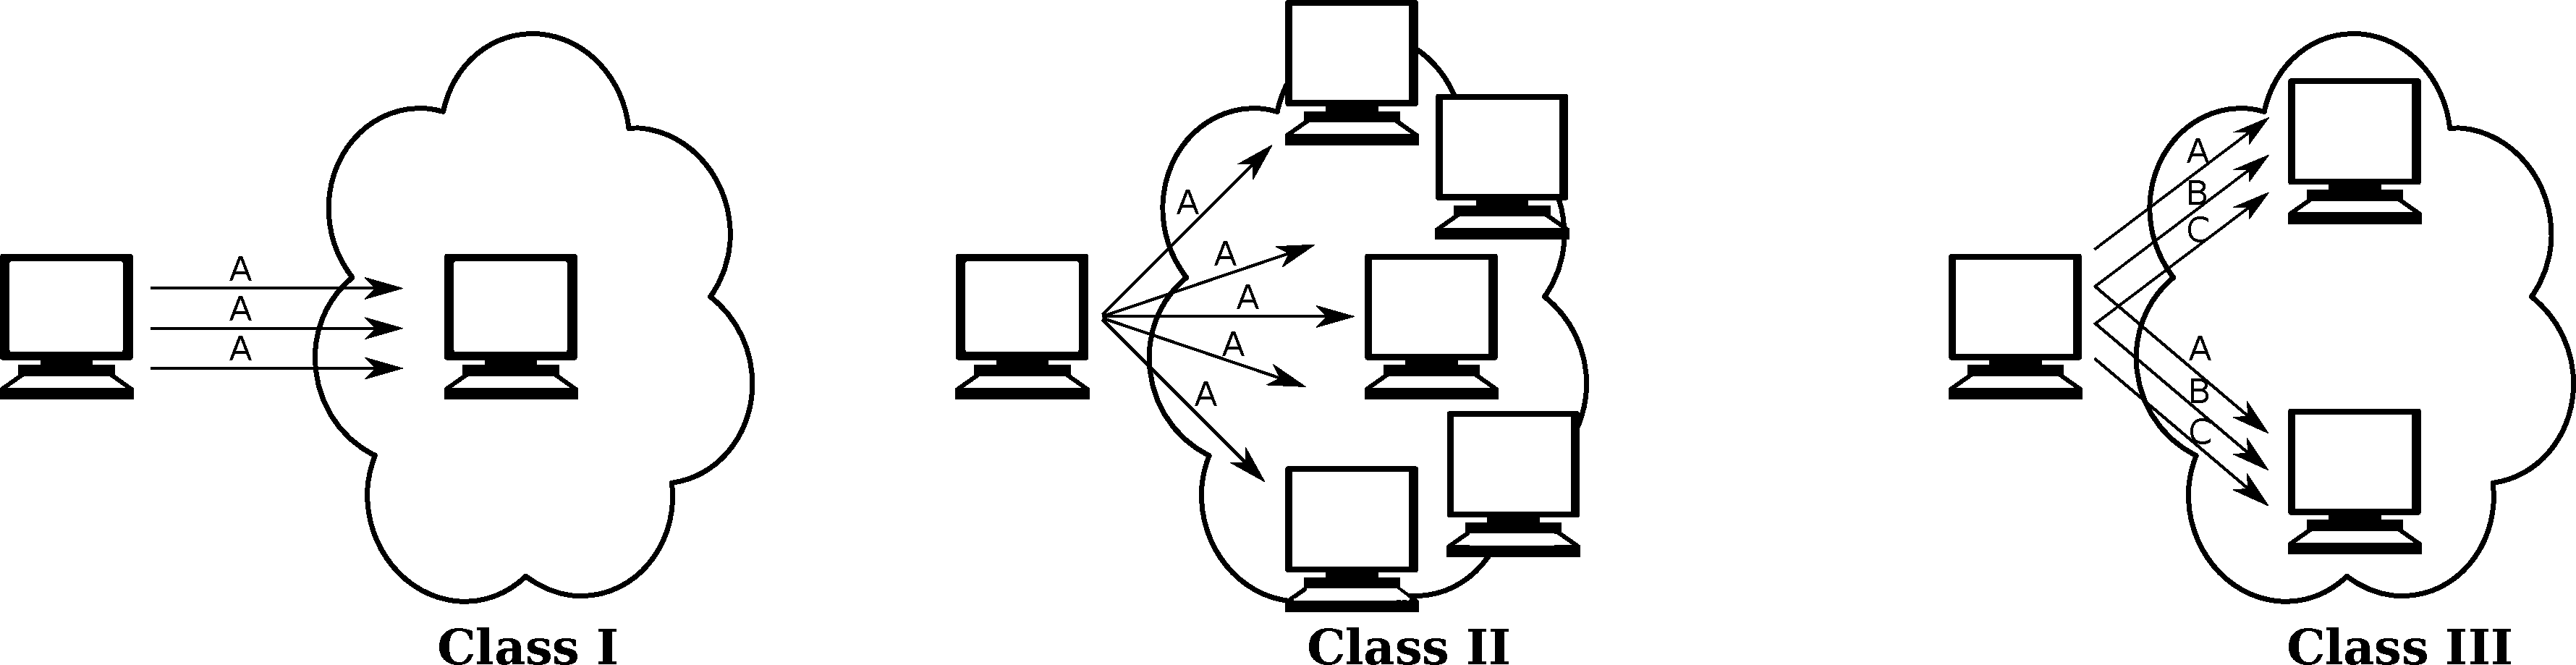
\includegraphics[width=\textwidth]{figures/paper-httpsecurity/classes}
  \caption{Selected Classes of HTTP Traffic}
  \label{fig:httpsecurity-classes}
\end{figure}


We were particularly interested in the results of three queries. First, how many similar requests were demanded by one source IP to one destination IP? Second, how many destination IP addresses were contacted by one source IP address with the same request? And third, how many requests were demanded by one source IP to one destination IP? Each query is represented by a class, as shown in Table~\ref{tab:httpsecurity-classes}. The classes correspond to patterns in the network traffic as depicted in Figure~\ref{fig:httpsecurity-classes}. A detailed description of each query and class can be found in the following subsections.

There are many other possible classes, although we found them to not be relevant from a security perspective. For example, many guests accessing a single host with a request suggests the popularity of a resource at the host. Such classes, however, could be interesting for general traffic classification, not security analysis.

\subsubsection{Class I: Repeated requests}

The first query asks for repeated requests between one guest and one host. We measured the number of occurrences of each triple, consisting of source IP, destination IP, and requested URL. Our assumption was that the repetition itself is common, but outstanding numbers may point to undesired behaviour. For example, password-protected web services may be exposed to brute-force attacks, which we can observe as a series of similar requests. The repeated request (A) is defined as follows:
\begin{equation*}
\begin{split}
Repeated&Request(A) \iff A = \{F \mid \forall F, F':\\
&F(srcip) = F'(srcip) \: \land \: F(dstip) = F'(dstip)\\
&\land \: F(path) = F'(path)\} \: \mbox{ and } |A| > threshold
\end{split}
\end{equation*}
All flows in the set share the same source IP address, destination IP address, and requested HTTP path. The total number of flows in the set is bigger than the threshold.

Sample results are presented in Table~\ref{tab:httpsecurity-repeat} from one day in summer 2014. As we can see, the numbers of repeated flows reaches tens of thousands, which represents outstanding traffic patterns. There is a disproportion in the numbers of flows with the same source IP, destination IP, and HTTP request. While the majority of the triples were unique or repeated several times, a small number of triples were observed to be repeated several thousand times or more. The nature of these repeated requests was revealed by analysing the request. The majority of repeated requests contained a substring such as \textit{admin} or \textit{login}, which suggests that these traffic patterns were caused by brute-force attacks against password-protected web services. Other interesting repeated requests contained the substring \textit{proxy}, which suggests communication between a client and a web-based proxy server. Furthermore, we found other repeated requests accessed large downloadable files, e.g., ISO images of Linux distributions.

\begin{table}[ht]
\centering
\begin{tabular}{| c | c | l | r|} \hline
Guest & Host & HTTP Path & \#Flows \\ \hline
G1  & H1 &                 /wp-\textbf{login}.php & 46,031 \\ \hline
G2  & H2 &      /\textbf{admin}istrator/index.php & 27,965 \\ \hline
G3  & H2 &      /\textbf{admin}istrator/index.php & 27,798 \\ \hline
G4  & H3 &                 /wp-\textbf{login}.php & 25,316 \\ \hline
G5  & H4 & \parbox[t]{5cm}{/pub/linux/slax/Slax-7.x/7.0.8/slax-Chinese-Simplified-7.0.8-i486.iso} & 5,921 \\ \hline
G6  & H5 &           /\textbf{proxy}/lib\textbf{proxy}.pac & 5,036 \\ \hline
G7  & H6 &                        /node/ & 4,286 \\ \hline
G8  & H4 & \parbox[t]{5cm}{/pub/linux/slax/Slax-7.x/7.0.8/slax-English-US-7.0.8-i486.zip} & 4,170 \\ \hline
G9  & H7 &                 /wp-\textbf{login}.php & 3,632 \\ \hline
G10 & H7 &           /polit/wp-\textbf{login}.php & 3,632 \\ \hline
\end{tabular}
\caption{Top Repeated Requests from One Day (Data Set Summer 2014)}
\label{tab:httpsecurity-repeat}
\end{table}

The second sample of results presented in Table~\ref{tab:httpsecurity-repeat2} was observed in one day in spring 2015. As we can see, there is a significant difference in the number of flows. However, the distribution of various types of repeated request is similar. One interesting anomaly is the guest G3, which performed repeated requests on 8 different hosts. This guest used different requests on different hosts, however the number of flows on each host is similar.

\begin{table}[ht]
\centering
\begin{tabular}{| c | c | l | r|} \hline
Guest & Host & HTTP Path & \#Flows \\ \hline
G1  & H1 & /\textbf{proxy}/lib\textbf{proxy}.pac & 5,147 \\ \hline
G2  & H2 & \parbox[t]{5cm}{/pub/linux/fedora/epel/6/x86\_64/repodata/ e63d28ff5a765b11a7052496f481f31aebab\\17c28545908d54e65904a1046ec8-filelists.sqlite.bz2} & 4,244 \\ \hline
G3  & H3 & /senat/studenti/wp-\textbf{login}.php & 3,992 \\ \hline
G3  & H4 & /\textbf{admin}istrator/index.php & 3,945 \\ \hline
G3  & H5 & /slovnik/\textbf{admin}istrator/index.php & 3,934 \\ \hline
G3  & H6 & /\textbf{admin}istrator/index.php & 3,926 \\ \hline
G3  & H7 & /capv2011/\textbf{admin}istrator/index.php & 3,924 \\ \hline
G3  & H8 & /index.php & 3,921 \\ \hline
G3  & H9 & /\textbf{admin}istrator/index.php & 3,794 \\ \hline
G3  & H10 & /wp-\textbf{login}.php & 3,701 \\ \hline
\end{tabular}
\caption{Top Repeated Requests from One Day (Data Set Spring 2015)}
\label{tab:httpsecurity-repeat2}
\end{table}

As we can see in Table~\ref{tab:httpsecurity-repeat-statistics}, which displays statistics for the whole monitored time window, almost half of the detected events were related to using a proxy. Brute-force password attacks were recognized only in 10.6\,\% of events. On the other hand, brute-force password attacks may generate more flows than other events in this class. They were the only events which generated more than 10,000 flows with the same source IP, destination IP, and HTTP path. However, we have also observed brute-force attacks of approximately a few thousand flows, but targeting multiple hosts over a short period of time.

\begin{table}[ht]
\centering
\begin{tabular}{l l r}
Subclass & Path regular expression & Portion [\%] \\
\hline
\textbf{Proxy} & & \textbf{49.4} \\
& .*libproxy.pac & 45.0 \\
& .*sviproxy.pac &  4.3 \\
& .*proxy.php    &  0.1 \\
\hline
\textbf{Brute-force} & & \textbf{10.6} \\
& .*admin.*            &  6.7 \\
& .*login.*            &  3.9 \\
\hline
\textbf{Others} & & \textbf{40.0} \\
\end{tabular}
\caption{Distribution of Repeated Request}
\label{tab:httpsecurity-repeat-statistics}
\end{table}

\subsubsection{Class II: Similar requests on many hosts}

The second query addresses identical requests from one source IP address to many destination IP addresses. Our assumption was that a guest accesses only a limited number of hosts or at least requests different paths from different hosts. Therefore, a guest accessing a large number of hosts with the same request (with the exception of ``/'') is suspicious and worth noting. We would also like to point out the similarity between this traffic pattern and network port scanning, e.g., TCP SYN scan~\cite{Bhuyan-2011-Surveying}. Therefore, we propose the name HTTP scan for this traffic class. HTTP scan (B) is defined as follows:
\begin{equation*}
\begin{split}
HTTP&Scan(B) \iff B = \{F \mid \forall F, F':\\
&F(srcip) = F'(srcip) \: \land \: F(dstip) \neq F'(dstip)\\
&\land \: F(path) = F'(path) \} \mbox{ and } |B| > threshold
\end{split}
\end{equation*}
All flows in the set share the same source IP address and requested HTTP path, while there are no flows with the same destination IP address. The total number of flows in the set is bigger than threshold.

First, we analysed only the scans of our monitored network by external hosts. Sample results from one day in summer 2014 are displayed in Table~\ref{tab:httpsecurity-scanners}. For each scan we state a guest, i.e., the scanner, the requested HTTP path, the number of visited hosts, and the percentage of visited hosts of all hosts in the monitored network. There were two outstanding source IP addresses identified, one accessed almost all the web servers in our network and requested six paths. The second scanner accessed significantly less hosts with only one requested path. The other combinations of Source IP address and path, including the ``/'' request, were not observed to access more than ten hosts a day. We observed up to nineteen events a day in the measurement, including events where a guest requested more than one path. The same paths were also observed to be requested by different guests.

\begin{table}[ht]
\centering
\begin{tabular}{| c | l | c | r |} \hline
Guest & HTTP Path & \#Hosts & \% \\ \hline
G1 & /myadmin/scripts/setup.php                 & 497 & 100 \\ \hline
G1 & /pma/scripts/setup.php                     & 497 & 100 \\ \hline
G1 & /w00tw00t.at.blackhats.romanian.anti-sec:) & 497 & 100 \\ \hline
G1 & /phpmyadmin/scripts/setup.php              & 495 &  99 \\ \hline
G1 & /phpMyAdmin/scripts/setup.php              & 494 &  99 \\ \hline
G1 & /MyAdmin/scripts/setup.php                 & 491 &  99 \\ \hline
G2 & /manager/html                              & 118 &  24 \\ \hline
\end{tabular}
\caption{Top HTTP Scanners from One Day (Data Set Summer 2014)}
\label{tab:httpsecurity-scanners}
\end{table}

The number of detected HTTP scans varied from 3 to 19 per day over the monitored time window. Ten scans per day were detected on average and scanning for multiple paths was common. The scan for six paths, displayed in Table~\ref{tab:httpsecurity-scanners}, was observed from four different IP addresses in one week. The other multiple-path scans did not use more than three paths in one scan.

The second sample results are from one day in spring 2015. We can see an interesting similarity of request in the first and second classes. The guest G1 was scanning for HTTP paths which also appeared in the results of the previous class. This suggests that the first class includes brute-force attacks and the second class some sort of network reconnaissance. Therefore, we may have observed the two phases of a complex attack.

\begin{table}[ht]
\centering
\begin{tabular}{| c | l | c | r |} \hline
Guest & HTTP Path & \#Hosts & \% \\ \hline
G1 & /wordpress/wp-login.php & 337 & 68 \\ \hline
G1 & /site/wp-login.php & 335 & 67 \\ \hline
G1 & /wp-login.php & 332 & 67 \\ \hline
G1 & /blog/wp-login.php & 201 & 40 \\ \hline
G2 & /bins.php & 183 & 37 \\ \hline
G3 & /cgi-bin/test-cgi & 102 & 21 \\ \hline
\end{tabular}
\caption{Top HTTP Scanners from One Day (Data Set Spring 2015)}
\label{tab:httpsecurity-scanners2}
\end{table}

Second, we searched for the HTTP scans in the opposite direction, i.e., scanning external networks by a host from our network. The detection in this direction is tricky as there are no clear boundaries of scanned networks and it is hard to set an appropriate threshold. In addition to this, even a common user may generate hundreds of similar requests such as \textit{/favicon.ico}. Therefore, we do not present any significant results. However, it would be possible to identify a scan by searching for continuous scanned network segments or the longest common prefix of the scanned IP addresses to estimate a scan of a subnet.

\subsubsection{Class III: Varying multiple requests on multiple hosts}

The third query addressed the guests which requested a large number of unique paths on a single host. In this case, we seek guests which requested the majority of content from our hosts. Our assumption is that a large number of different requests from one guest to one host is a legitimate traffic pattern. On the other hand, outstanding numbers worth noting can also be observed. Then we looked for guests which requested an outstanding number of unique paths on more than one host. We assume that only crawlers behave in this way and it is unusual that any other guest would request such a large number of unique URLs on more hosts. The activity of a crawler (C) is defined as follows:
\begin{equation*}
\begin{split}
Crawler&Candidate(C') \iff C' = \{F \mid \forall F, F':\\
&F(srcip) = F'(srcip) \: \land \: F(dstip) = F'(dstip)\\
&\land \: F(path) \neq F'(path)\} \: \mbox{ and } |C'| > threshold_1
\end{split}
\end{equation*}
\begin{equation*}
\begin{split}
Crawler&(C) \iff C = \{F \mid \forall C^\prime_i, C^\prime_j:\\
&F_i \in C^\prime_i \land F_j \in C^\prime_j \land F_i(srcip) = F_j(srcip)\}\\
&\mbox{and } |C| > threshold_2
\end{split}
\end{equation*}
We detect crawlers as guests which requested many resources from more hosts. First, all flows which have the same source IP address and destination IP address, but distinct requested HTTP paths, are grouped to sets. The first threshold is a minimal number of distinct requests on a single host. Second, we select source IP addresses which appeared in more sets. The second threshold is a minimal number of crawled hosts. The thresholds were selected to include at most 10\,\% of sets.

In the first phase, we confirmed that the assumed traffic pattern occurs frequently with a varying number of requested URLs. We were not able to unambiguously mark outstanding numbers. In the second phase, we filtered out the guests which did not access more than one host. The remaining guests were characterized by common signs, e.g., they accessed similar sets of hosts and requested a similar number of URLs. We have marked these guests as crawlers and present sample results from a one-day measurement in Tables~\ref{tab:httpsecurity-crawlers} and \ref{tab:httpsecurity-crawlers2}.

\begin{table}[ht]
\centering
\begin{tabular}{| l | l | c |} \hline
Guest & Domain Name & \#Hosts \\ \hline
207.46.13.62    & msnbot-207-46-13-62.search.msn.com  & 7 \\ \hline
157.55.39.107   & msnbot-157-55-39-107.search.msn.com & 6 \\ \hline
137.110.244.137 & bnserver2.sdsc.edu                  & 4 \\ \hline
157.55.39.156   & msnbot-157-55-39-6.search.msn.com   & 4 \\ \hline
157.55.39.6 & msnbot-157-55-39-156.search.msn.com & 4 \\ \hline
37.187.28.19    & z3.sentione.com                     & 4 \\ \hline
137.110.244.139 & integromedb-crawler.integromedb.org & 3 \\ \hline
5.135.154.106   & nks02.sentione.com                  & 3 \\ \hline
5.135.154.98    & nks03.sentione.com                  & 3 \\ \hline
77.75.73.32 & fulltextrobot-77-75-73-32.seznam.cz & 3 \\ \hline
77.75.77.17 & fulltextrobot-77-75-77-17.seznam.cz & 3 \\ \hline
% 151.228.8.115 & 97e40873.skybroadband.com           & 2 \\ \hline
% 157.55.39.13  & msnbot-157-55-39-13.search.msn.com  & 2 \\ \hline
% 157.55.39.155 & msnbot-157-55-39-155.search.msn.com & 2 \\ \hline
% 157.55.39.184 & msnbot-157-55-39-184.search.msn.com & 2 \\ \hline
% 5.255.253.60  & spider-5-255-253-60.yandex.com      & 2 \\ \hline
% 77.75.77.32   & fulltextrobot-77-75-77-32.seznam.cz & 2 \\ \hline
\end{tabular}
\caption{Top HTTP Crawlers from One Day (Data Set Summer 2014)}
\label{tab:httpsecurity-crawlers}
\end{table}
% requests per host? zajimave pro implementaci

Out of 11 crawlers detected in one day in summer 2014, 4 were identified as a well-known MSN search bot. The others were mostly local search engines, i.e., the Czech search engine Seznam (2 guests) and social media monitoring tool Sentione (3 guests). The two remaining guests were identified as a part of an IntegromeDB crawler collecting biomedical data.

The second sample results are based on a one-day measurement in spring 2015. In the course of this day, we detected a higher activity of crawlers in our network. The recognized crawlers accessed significantly more hosts and generated more unique HTTP requests. We mostly observed well-known crawlers, such as the MSN search bot and two local search engines. One interesting finding was the detection of an unknown guest behaving like a crawler. The guest's IP address had no reverse domain name assigned and its WHOIS record pointed to a hosting company, which indicates a potentially malicious crawler.

\begin{table}[ht]
\centering
\begin{tabular}{| l | l | c |} \hline
Guest & Domain Name & \#Hosts \\ \hline
157.55.39.97  & msnbot-157-55-39-97.search.msn.com  & 24 \\ \hline
207.46.13.11  & msnbot-207-46-13-11.search.msn.com  & 23 \\ \hline
157.55.39.28  & msnbot-157-55-39-28.search.msn.com  & 18 \\ \hline
157.55.39.209 & msnbot-157-55-39-209.search.msn.com & 17 \\ \hline
157.55.39.41  & msnbot-157-55-39-41.search.msn.com  & 15 \\ \hline
195.113.155.3 & severus.mzk.cz & 11 \\ \hline
77.75.77.123  & screenshotgenerator-77-75-77-123.seznam.cz & 11 \\ \hline
77.75.77.200  & screenshotgenerator-77-75-77-200.seznam.cz & 11 \\ \hline
46.229.164.99 & NOT FOUND & 10 \\ \hline
\end{tabular}
\caption{Top HTTP Crawlers from One Day (Data Set Spring 2015)}
\label{tab:httpsecurity-crawlers2}
\end{table}

Similarly to HTTP scans, we were looking for the described activity in the opposite direction, i.e., crawling of external web servers by a crawler from our network. Again, the detection in the opposite direction is harder as there no clear thresholds and many potential false positives. The thresholds for crawler detection had to be set considerably higher to avoid false positives. However, no significant results demonstrating the advantages of this method were found.


\subsection{Discussion}\label{subsec:httpsecurity-discussion}

In previous section we outlined three relevant classes of network traffic. The classes cover similar traffic patterns and can be characterized by outstanding numbers of observed network flows. The first class revealed several interesting patterns with ambiguous results as it can be split into several subclasses according to the HTTP request used. The second class is assumed to be solely malicious as it contains scanning for application vulnerabilities. The third class is considered mostly legitimate and is assumed to cover the activity of search bots and crawlers. However, not all the bots and crawlers are welcome in the network. Impacts on network security and the confirmation of the assumptions are discussed in this section for each class. There is also an interesting correlation between the first and second class which suggests that the malicious activity may be observed in both classes.

\subsubsection{Class I: Brute-forcing and proxy servers}

The first class is characterized by a large number of the same HTTP request from one guest to one host. As we can see in the results, several types of network activity are covered by this class. Generally, we cannot distinguish between them by the number of observed flows. The subclasses are easily distinguishable by analysing the requested path.

The first subclass was observed most often and was identified as communication between client and proxy. This subclass can be easily recognized by the substring \textit{proxy} in a requested path. All the detected hosts were legitimate proxy servers in our network. The clients were located in networks of ISPs in our country, so we suppose the clients were legitimate. The implication for network security monitoring in this case is the possibility of proxy detection. We are able to detect active proxy servers in the network and identify their clients. Therefore, we should be able to reveal illegitimate proxy servers in the network or the illegitimate use of a proxy by unauthorized clients, e.g., from networks with a bad reputation~\cite{MoreiraMoura-2013-Internet}.

The second subclass was not observed often, but generated the record number of flows. Paths containing a substring such as \textit{admin} or \textit{login} suggest a request to a resource protected by authentication. Paths ending in \textit{wp-login} indicate the presence of an administrative interface of a well-known content management system WordPress, which is prone to brute-force password attacks~\cite{WordPressCodex-2014-Brute}. This path was observed very often and the high number of flows, typically over a short period of time, indicates an attack. We accessed the requested URLs and confirmed that the hosts are running WordPress and provide a login page at the requested path. Another well-known content management system, Joomla!, was also a target of brute-force password attacks. The login page of Joomla! is located under a generic-looking path \textit{/administrator/index.php} and we have confirmed the presence of Joomla! at the observed URLs.

An interesting conclusion is that the dictionary attacks are rarely accompanied by any other network traffic from the source IP address. There were neither scans nor any other access to the host preceding the attack as is common among SSH brute-force attacks~\cite{Vykopal-2013-Flow}. We suppose this is due to attackers using a ``Google Hacking'' technique~\cite{Billig-2008-Evaluation}. In this technique, a search engine (e.g. Google, hence the name) is abused to do the reconnaissance for the attacker. The attacker searches a string typical for a WordPress login page and the search engine returns a list of WordPress instances which can be accessed instantly. Several well-aimed Google searches proved this assumption.

Although we can easily identify the two subclasses by the presence of characteristic substrings, the group of requested path is uncategorized and creates a third subclass. Paths such as \textit{/node/} and \textit{/wiki/} do not indicate a vulnerable resource. Dynamically generated content was observed on the requested URLs which suggests that the requests were legitimate. Highly repeated requests for URLs of files for downloading can be explained by partitioning the download, e.g., by download managers, and, thus, is legitimate traffic.

\subsubsection{Class II: HTTP scanners}

The second class was marked as HTTP scanning. Requested paths suggest that the scanning guests are searching for specific web applications and their vulnerabilities. It is also common that more paths, versions, or applications are probed during one scan. This type of traffic is easily detectable and highly interesting from a network security perspective. We have not observed any traffic that could be mistaken for a scan or marked as a false positive in this class. Even the low threshold of scanned hosts is sufficient for detection of a scanner as not every scanner accesses every host in the network. Fairly good results can be achieved with a threshold set to one fifth of the number of web servers in the network.

The HTTP scans were further analysed and correlated to TCP SYN scans on port 80. The results confirm the malicious nature of the scans. 46 \% of the HTTP scans were preceded or accompanied by a TCP SYN scan of the full range of our network. The first option is that the scanner first obtains the list of IP addresses with port 80 opened and then scans them with HTTP requests. The delay between the two phases varies from one hour to several days. The second option of HTTP scanning is to send a HTTP request instantly after receiving a response to the TCP SYN packet.

TCP SYN scanning is easily detectable using network flow monitoring~\cite{Sperotto-2010-Overview}, but scanners can avoid detection by scanning ``low \& slow''~\cite{Kang-2007-Distributed}. We propose using application flow monitoring to increase the detection rate of network scanning and lower the amount of false positives. We observed scanners that scanned no more than 5,000 IP addresses out of a /16 network range with a TCP SYN packet and continued HTTP scanning the web servers they found. Naturally, the scanners did not scan all the web servers, they typically found 100--250 hosts. On the other hand, as we stated earlier, more than 100 scanned hosts is enough to identify a scanner, at least in a network containing around 500 web servers. Therefore, we are able to identify a scanner which would otherwise avoid detection due to the high threshold of the TCP SYN scan detection method.

Another interesting property of the HTTP scans is that some of the requested HTTP paths were observed as a target of brute-force attack as well. For example, the scanners were looking for running instances of WordPress by requesting paths ending in \textit{wp-login}. The same paths were subjects of thousands of repeated request, which we consider as a brute-force attack. This lead us to suggestion that the attackers search for victim of a brute-force attack using the HTTP scans, just like it is common for attackers to perform port scan before a brute-force attack against services such as SSH~\cite{Vykopal-2013-Flow}.

\subsubsection{Class III: Web crawlers}

The third recognized class of HTTP traffic was marked as crawlers. The query had to be further specified due to the interchangeability of crawlers and common guests when measured on a single host. Covering more hosts in the network provided us with a set of crawlers active in our network. The crawlers were further analysed to filter out false positives. Filtering methods consisted of querying reverse DNS records, querying the WHOIS database, and checking User-Agents used in HTTP requests. We confirmed the identified set was populated by legitimate crawlers. The User-Agents in the HTTP headers pointed to well-known search engines such as Googlebot, Bing, and Baidu. Reverse DNS and WHOIS records further confirmed the presumptions by referring to domains names of the search engine owners.

Crawlers are mostly legitimate and welcome in the network~\cite{Sun-2010-Ethicality}. Almost all the crawlers we discovered were confirmed as legitimate. However, there are two reasons why we included them in a security-related analysis. First reason is small number of IP addresses that were identified as crawlers using the flow-based method, but we were not able to tell which any further information about them. Missing reverse DNS records or empty User-Agent fields in HTTP queries lead to suggestion that these IP addresses performed illegitimate crawling, e.g., e-mail harvesting that aims at discovering spam recipients~\cite{Hohlfeld-2012-Longtime}.

The second reason of including crawlers in the analysis is the large number of flows they generate. Any potential detection method based on application flow analysis would have to deal with false positive alerts. Legitimate web crawlers can be easily mistaken for malicious traffic due to their omnipresence and large number of requests. On the other hand, we have to be careful about false negatives, i.e., malicious hosts disguising as crawlers to avoid attention. In addition to this, operators of web crawlers may change the addresses of their bots over time or not publish them at all, which makes creating a whitelist a difficult task. Our method is based on monitoring the behaviour of the potential crawler, which alleviates the possibility of false positives or false negative detections. The User-Agent field of HTTP application flow record can also be used for validation of the results.


\subsection{Conclusion}\label{subsec:httpsecurity-conclusion}

We presented an analysis of HTTP traffic using application flow monitoring in a large campus network. Contrary to previously published analyses, we were the first to focus on the security aspects.
We identified three security-related traffic classes: repeated requests, HTTP scans, and web crawlers. Repeated request were further split into brute-force password attacks and proxies according to the observed HTTP request.

This classification is based on an analysis of selected elements of application flow: source IP, destination IP, and requested URL split into domain and path.
Our analysis supported the hypothesis that flow application monitoring with HTTP headers (Layer 7) enables the straightforward detection of current security issues compared to basic flow monitoring performed at Layers 3 and 4. Particularly, the brute-force password attacks and proxies are hard to differentiate using only basic flow monitoring.

Malicious traffic is contained in the classes of HTTP scans and repeated request, in which we were able to identify brute-force attacks against well-known content management systems. Web crawlers represent a class of legitimate traffic that can be mistaken for malicious activity due to its large number of generated flows. However, suspicious crawlers can also be observed. We have also identified the use of proxies as a traffic class. Using a proxy is not malicious by nature, but is interesting for security enforcement. For example, the presence of an unauthorized proxy may violate security policy in the network.

The classification is based on counting number of application flows which share one or more parameters. The classification can be thus easily converted into a threshold-based detection method. 
We were able to detect malicious HTTP traffic in large-scale network and process it from one point with a low amount of false positives. Ten previously undetectable brute-force password attacks and 10 HTTP scans per day were detected on average in our campus network. In addition, previously unknown proxies and web crawlers were observed. 
The large-scale network monitoring approach proved beneficial particularly during the detection of HTTP scans and web crawlers, which are hardly detectable using only local system logs or local monitoring.

Further work will involve the integration of the proposed methods into the existing detection framework in the campus network. False positive and false negative ratios of the detection methods based on our proposed methods will be evaluated. The security incidents concerning HTTP will be resolvable globally in the whole network and the security awareness can be spread more effectively. 
Additionally, we will use the discovered classes for setting up more efficient honeypots to respond to the requested vulnerability. This applies particularly to HTTP scanners and brute-force password attacks. We should be able to equip a honeypot with an appropriate resource, e.g., vulnerable web application that the adversaries were looking for, to attract and analyse specific attacks. 
The honeypot use case involves both network monitoring and security incident analysis and can lead to an effective reaction to upcoming threats including a reaction to zero-day attacks.

%%%%%%%%%%%%%%%%%%%%%%%%%%%%%%%%%%%%%%%%%%%%%%%%%%%%%%%%%%%%%%%%%%%%%%%%%%%%%%%%%%%%%%%%%%%%%%%%%%%

\section{An Investigation Into Teredo and 6to4 Transition Mechanisms: Traffic Analysis}\label{sec:analysis-ipv6-transition}

Despite IPv6 being the standard for several years its adoption is still in process~\cite{Claffy-2011-Tracking}. There are several ways of getting IPv6 connectivity, the dual-stack being the preferred one. Most IPv6 studies deal with native IPv6. However, there are other globally used options known as transition mechanisms. They can provide IPv6 connectivity on networks without native IPv6 connectivity enabled or without an IPv6 ready infrastructure.

The transition mechanisms tunnel IPv6 traffic through IPv4 network. Despite being supported by major operating systems, there is a lack of studies investigating the characteristics of the tunneled IPv6 traffic. In this context, this section investigates border traffic of the Czech national research and education network operator (CESNET) and attempts to answer the following question: \emph{What are the characteristics of IPv6 transition mechanisms, in terms of their usage, popularity and impact on native IPv4 and IPv6?}

Our research is mainly motivated by an exhaustion of the IPv4 address space and an exerting pressure on network operators and content providers to deploy IPv6. The transition mechanisms are used to facilitate the IPv6 adoption. Unfortunately, they introduce extra elements in the network which add to complexity and decrease performance and security. As a result, many existing methods for measuring and monitoring large-scale networks become ineffective.

The contribution of our work is threefold: Firstly, we provide an enhanced version of our flow-based IPv6 measurement system prototype, which enables IPv6 visibility in large-scale networks. Secondly, we analyze and show IPv6 transition mechanisms traffic characteristics including a tunneled one and thirdly, we show how the traffic of IPv6 transition mechanisms has evolved since 2010.

The section is organized as follows. Subsection~\ref{subsec:ipv6-tunnels-related-work} outlines related work. Subsection~\ref{subsec:ipv6-tunnel-traffic} provides an overview of Teredo and 6to4 transition mechanisms. Subsection~\ref{subsec:ipv6-tunnels-met-mon-setup} describes the methodology and measurement setup. Subsection~\ref{subsec:ipv6-tunnels-outer-traffic-evaluation} investigates properties of IPv4 traffic carrying IPv6 payload. Subsection~\ref{subsec:ipv6-tunnels-inner-traffic-evaluation} focuses on the characteristics of encapsulated IPv6 traffic. Subsection~\ref{subsec:ipv6-tunnels-evaluation-of-ipv6} evaluates the use of IPv6 tunneled traffic. Finally, we draw conclusions in Subsection~\ref{subsec:ipv6-tunnels-conclusion}.

\subsection{Related Work} \label{subsec:ipv6-tunnels-related-work}

The most widely used and discussed tunneling transition mechanisms are Teredo and 6to4. Although there are several studies focusing on performance evaluation of transition mechanisms listed below, the characteristics of the traffic generated by the tunneling transition mechanisms are not well known.

A study by~\citeauthor{Aazam-2010-Comparison}~\cite{Aazam-2010-Comparison} provides a performance evaluation and a comparison of Teredo and Intra-Site Automatic Tunnel Addressing Protocol (ISATAP) mechanisms with focus on certain parameters like throughput, end to end delay, round trip time and jitter. A study by~\citeauthor{Zander-2012-Investigating}~\cite{Zander-2012-Investigating} compares Teredo tunneling capability and performance with native IPv6 and 6to4 using measurements related to web services. Teredo increases the time needed to fetch web objects compared to IPv4 or native IPv6. The conclusion is that Teredo seems to be limited by a lack of Teredo infrastructure forcing encapsulated packets to travel long distances. Moreover, the throughput is partially limited by the performance of Teredo relay servers.

A study by~\citeauthor{Bahaman-2012-Network}~\cite{Bahaman-2012-Network} discusses the performance of 6to4 with focus on communication over TCP. It states that the TCP transmission ability is reduced by the use of 6to4. However, it is still suitable for early stages of the transition period.

Other papers discuss the impact of transition tunnels on network security. Krishnan et al.~\cite{rfc6169} present security concerns with recommendations on how to minimize security exposure due to tunnels. It is pointed out that tunnels can have negative impact on deep packet inspection and that transition mechanisms such as Teredo allow inbound access from the public Internet to a device through an opening created in a network address translation (NAT) device. This increased exposure can be used by attackers to effectively attack a device hidden behind a NAT device. A generally proposed security practice is to avoid the usage of tunnels at all and deploy other transition schemes like dual-stack.

Finally,~\citeauthor{Sarrar-2012-Investigating}~\cite{Sarrar-2012-Investigating} provides a brief insight into tunneled traffic in a study of the world IPv6 day impact on IPv6 traffic. The Teredo and 6to4 transition mechanisms were monitored and the Teredo was discovered to carry mainly control traffic. The study also showed that IPv6 fragments were responsible for a significant portion of 6to4 traffic. The authors suspect that these fragments were caused by broken software which most likely forgot to take the IPv6 header size into account.

\subsection{Investigated IPv6 Transition Mechanisms} \label{subsec:ipv6-tunnel-traffic}

The IPv6 traffic is usually divided between \emph{native} traffic and \emph{tunneled} traffic. The tunneled traffic is considered the one encapsulated using other protocols, e.g. UDP or IP protocol 41. This division is not necessarily accurate, since the traffic that seems to be native IPv6 can in fact originate from a client using some transition mechanism like Teredo or 6to4. To clarify this point we will differentiate between native IPv6 traffic, encapsulated tunnel traffic (IPv4 traffic containing IPv6 payload) and decapsulated tunnel traffic. The word tunnel might be omitted for the sake of brevity. 

Teredo and 6to4 are the two most frequently used transition mechanisms in the CESNET network. Mechanisms like ISATAP, Anything in Anything (AYIYA) and others based on IP protocol 41 (6in4, 6over4) do not contribute to the tunneled traffic significantly and do not appear in our analysis, therefore we will not describe them in detail. We did not analyze NAT64 and DNS64 mechanisms since they should appear as a native IPv6 traffic on the outside.

Teredo~\cite{rfc4380} is designed to provide IPv6 connectivity to an endpoint behind a NAT device. It requires two network components for operation: \emph{relays} and \emph{servers}. Teredo servers are used for initialization of Teredo (Figure~\ref{fig:ipv6-tunnels-monitoring-schema}, communication \ding{172}), and after that for opening a port on the user's NAT device in case of communication which is not initialized by the user. Relays are used for routing and bridging the IPv4 and IPv6 networks. Each Teredo endpoint uses a statically configured server and a relay, which can cause increased latency and low throughput in case of a distant server or relay. Teredo uses UDP for packet encapsulation making the traffic harder to identify.

6to4~\cite{rfc3056} is only suitable for hosts with a public IPv4 address. It uses encapsulation in IP protocol 41 packets hence it is relatively easy to detect and monitor. The 6to4 relay servers are acting as a bridge between the IPv4 and IPv6 networks. These relays use any-cast prefix 192.88.99.0/24 therefore the optimal (nearest) relay server should automatically be used for communication.

Figure~\ref{fig:ipv6-tunnels-monitoring-schema} shows traffic between two endpoints (communication \ding{175}), one of which uses Teredo and the other one 6to4. The IPv6 traffic from Teredo client travels part of its path in Teredo tunnel to be later decapsulated on the edge of IPv6 Internet and shortly after that to be encapsulated again, this time by 6to4 to travel the rest of its path over IPv4 Internet to the network of its destination. Depending on where the observation point is located, the tunnel (either Teredo or 6to4) or native IPv6 traffic can be observed.

\begin{figure}[!tb]
        \centering
        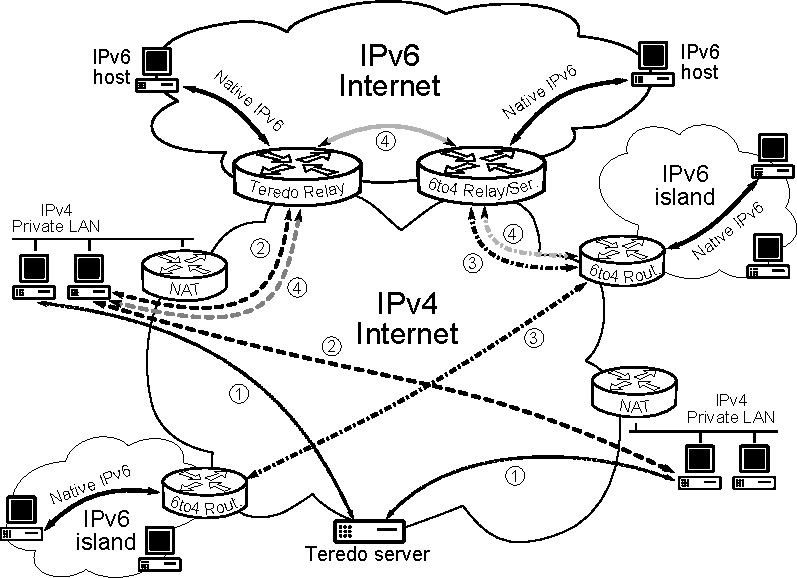
\includegraphics[width=1.00\linewidth]{figures/paper-tunnels/tunely-schema}
        \caption{Teredo and 6to4 Principles: \ding{172} Teredo Start Setup, \ding{173} Teredo Traffic Transiting over IPv4 Network, \ding{174} 6to4 Traffic Transiting over IPv4 Network, \ding{175} Communication between Teredo and 6to4 Endpoint}
        \label{fig:ipv6-tunnels-monitoring-schema}
\end{figure}

% Depending on where the observation point is stationed, the tunnel or native IPv6 traffic is observed.
% Most of the our analysis refers to encapsulated tunnel traffic, since we are able to analyze both encapsulating and encapsulated packet headers and therefore gain more extensive information.

\subsection{Methodology and Measurement Setup} \label{subsec:ipv6-tunnels-met-mon-setup}

To perform a thorough inspection of tunneled traffic, we need to decapsulate packet headers of inner packets. We use the same flow-based framework as in~\cite{Elich-2011-Monitoring} which has been further modified~\cite{Elich-2013-FlowMon} to extract more detailed information from tunneled data. The main part of the framework is a plug-in which replaces input and processing parts of existing flow generator FlowMon Exporter~\cite{FlowmonNetworks--Flowmon}. 
% The older version of framework extracted only a subset of fields the newer version is capable of. 

Every packet is being processed to extract basic flow statistics and the processing of inner headers continues to the point when previously extracted fields indicate absence of observed encapsulation types.

Teredo protocol is detected when IPv6 header is found encapsulated in UDP packet, AYIYA is searched for in packets on TCP or UDP port 5072. Other protocols are recognized by IPv6 address format, which is protocol specific and the 6to4 protocol can be additionally identified by usage of IPv4 anycast address belonging to 6to4 relay. If encapsulation is present, its type and encapsulated IPv6 header fields are used to extend the set of extracted fields and to identify individual flows taking place inside the tunnel. 

Since we need to define new elements for application flow records, Internet Protocol Flow Information Export (IPFIX) protocol is used. It allows using \emph{Enterprise Elements} which can extend the application flow records with additional tunnel information. 
The framework is able to recognize and extract information from Teredo, AYIYA and other protocols that are based on IP protocol 41 such as ISATAP, 6to4 and 6over4. 
We provide the source code of the measuring tool under BSD license at the project web page~\cite{Elich-2013-FlowMon}.

\begin{figure}[!tb]
\centering
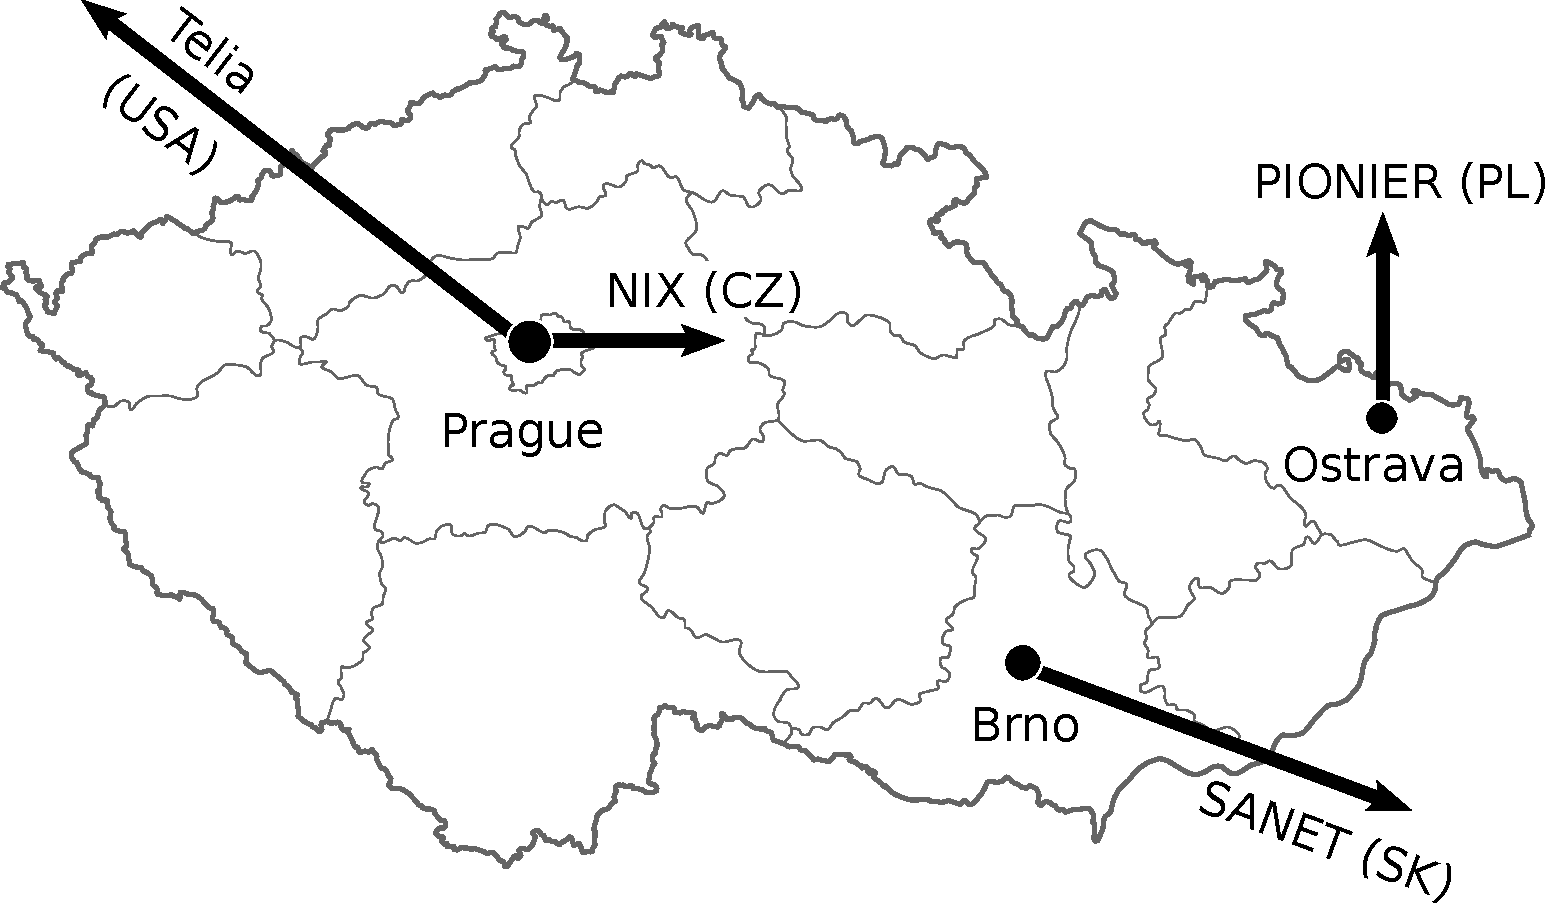
\includegraphics[width=0.9\linewidth]{figures/paper-tunnels/cesnet-map}
\caption{CESNET monitored links}
\label{fig:ipv6-tunnels-topology}
\end{figure}

\begin{table}[!tb]
\centering
        \begin{tabular}{lccc}
        \textbf{Probe} & \textbf{Bits/s} & \textbf{Packets/s} & \textbf{Flows/s} \\ \toprule 
        Telia & 1.65\,G & 274.9\,k & 22.1\,k \\
        NIX & 7.17\,G & 1072.4\,k & 26.7\,k \\
        PIONIER & 0.51\,G & 75.6\,k & 2.8\,k \\
        SANET & 1.87\,G & 242.3\,k & 5.3\,k \\ \bottomrule
        \end{tabular}
        \caption{Observation Points IPFIX Statistics}
        \label{tab:ipv6-tunnels-collected-data}
\end{table}

Resulting flow data provides us with information about the encapsulated source and destination addresses, ports and transport protocol, which is a common five-tuple used to distinguish individual flows. We respect this principle and thus have separated the flows encapsulated in the same tunnel based on the value of these elements. Apart from these key elements the framework gives information about \emph{Time to Live} (TTL), \emph{encapsulated HOP limit}, \emph{TCP flags} and \emph{ICMPv6 type} and \emph{code}, when present. Moreover, additional information about tunnel type is provided, including Teredo header and trailer types when present. The framework also newly supports geolocation using MaxMind~\cite{MaxMind-2013-MaxMind} GeoIP database for both outer and encapsulated addresses.

The data are collected from several observation points located at the borders of CESNET network by passive probes; see Figure~\ref{fig:ipv6-tunnels-topology}. All measured lines are at least 10\,Gbit/s and together transport about 80,000\,flows/s during work hours, which results in total traffic of 15.4\,Gbit/s. We use IPFIXcol~\cite{Velan-2012-Flow} framework to collect the extended flow data over TCP and to store them. New elements can therefore be defined and used without any further difficulties or limitations.

The IPFIX data was collected over one week in January 2013 without use of any sampling. Table~\ref{tab:ipv6-tunnels-collected-data} shows the average amount of traffic for all observation points. The total amount of stored data took approximately 2,485\,GB of disk space. All statistics presented below are based on flow count.

\subsection{Characteristics of IPv4 Tunnel Traffic} \label{subsec:ipv6-tunnels-outer-traffic-evaluation}

In this section we describe characteristics of IPv4 traffic containing IPv6 payload. The analysis is based purely on information from IPv4 headers and extended flow data are only used to accurately identify relevant flows. Three characteristics that can give us insight into tunneled traffic are addressed. Firstly, we describe TTL values of the various traffic sets, and then we look into a geolocation aspect. Lastly, the basic flow statistics are presented.

\subsubsection{Frequency of TTL and HOP Values}
We study the distribution of \textit{TTL values} of the observed flows. It is known that some operating systems use specific values, as shown in~\cite{Davids-2017-Initial}. Microsoft Windows has the default TTL set to 128. The value of 64 is mostly used by Mac~OS~X and Linux devices, including devices running Android. We expect that these operating systems form a majority and are therefore the most significant. Figure~\ref{fig:ipv6-tunnels-ipv4-ttl} shows the most frequently used TTL values for IPv4 flows carrying IPv6 payload. The TTL values are most frequent near the values set by OS vendors and the frequency is decreasing rapidly in less than ten hops. Therefore, we assume that most of the packets reach their destination in less than 32 hops. Thus we classify the flows according to their TTL numbers into four significant groups. The Windows traffic seems to be the most frequent one taking 60.3\,\% of the total, while Linux machines are not present so often with only 23.8\,\%. Apart from the Windows and Linux ranges, there are devices that set TTL to 255 and 32. Although the 255 are usually Cisco routers, in case of tunneled traffic we observed that the 6to4 traffic from anycast addresses have TTL set to 255 as well. The portion of the 255 range is 3.8\,\% and most of it originates from 6to4 relays. TTL numbers 24 and 26 are dominant in the group of values from 1 to 32, which makes 12.2\,\% of the total number of flows. We discovered that this is caused by a 6to4 tunnel that passes two observation points. The tunnel is heavily used and causes a large portion of tunneled traffic, which also affects other 6to4 measurements.

Overall, the TTL distribution of IPv4 traffic is different as shown in Figure~\ref{fig:ipv6-tunnels-ipv4-ttl4}. The Linux portion of the traffic is higher and the TTL values of 32 and 255 are not as significant. A more detailed examination of the flow records shows that this is caused mainly by a high ratio of HTTP traffic. Even though there are more clients using Windows operating system, most of the web servers are based on Linux and therefore the responses have TTL less than 64. The DNS protocol shows similar characteristics except that the DNS traffic that we observe at our metering points is mostly generated by recursive domain name servers. Since the Linux DNS servers are the most widely used, they significantly contribute to the traffic generated by Linux machines.

\begin{figure}[tb]
    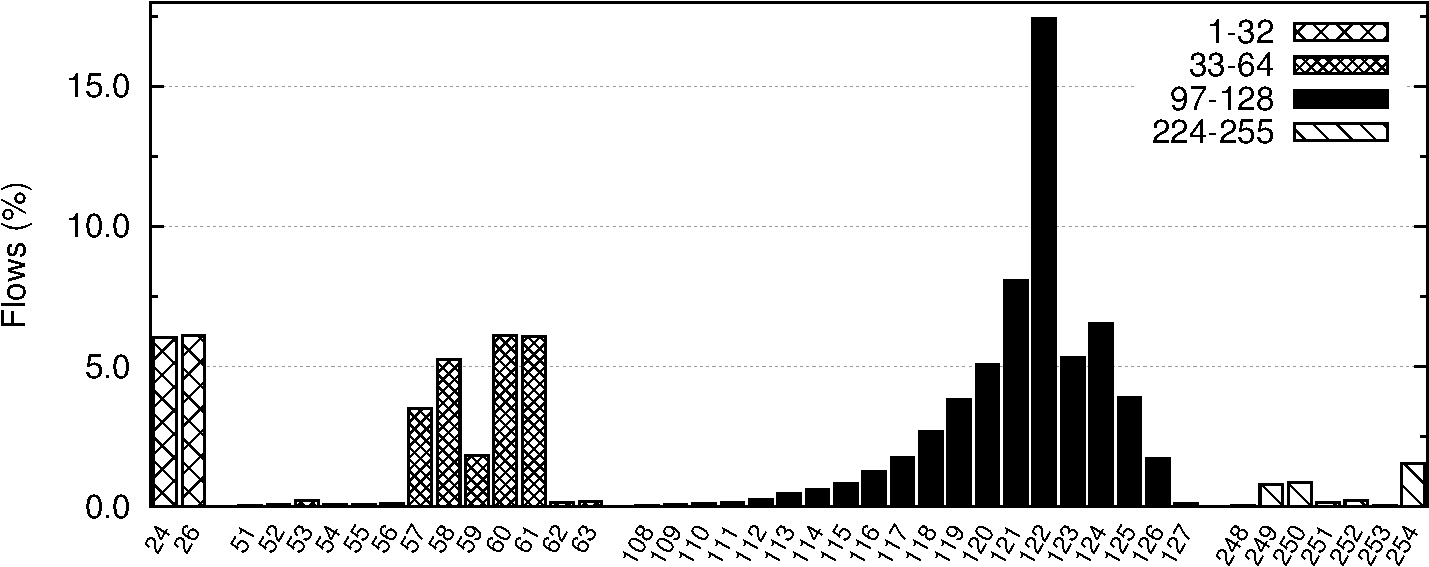
\includegraphics[width=1.00\linewidth]{figures/paper-tunnels/ttl/ttl}
    \caption{TTL Value Distribution of IPv4 Traffic Containing IPv6 Payload}
    \label{fig:ipv6-tunnels-ipv4-ttl}
\end{figure}

\begin{figure}[tb]
    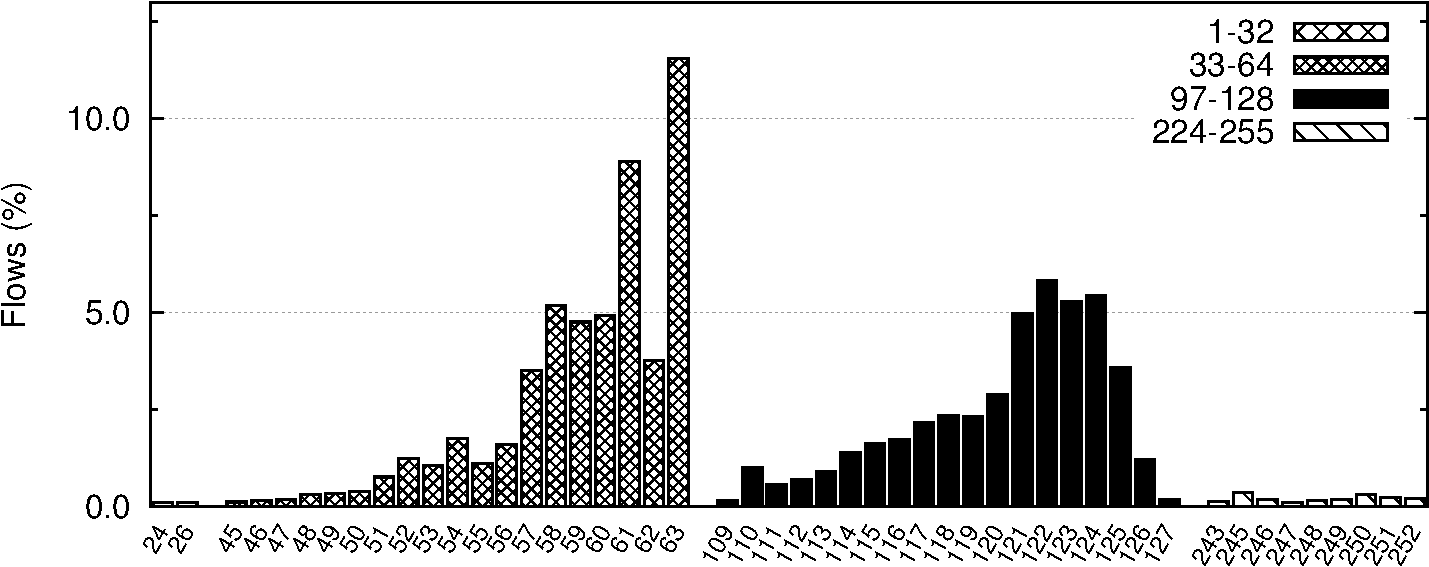
\includegraphics[width=1.0\linewidth]{figures/paper-tunnels/ttl/ttl4}
    \caption{TTL Value Distribution of Total Observed IPv4 Traffic}
    \label{fig:ipv6-tunnels-ipv4-ttl4}
\end{figure}

IPv6 uses \textit{HOP limit} instead of TTL. Figure~\ref{fig:ipv6-tunnels-ipv6-native-hop} shows HOP limit distribution of native and decapsulated IPv6 traffic. Unlike IPv4, the HOP limit of 64 is the most frequent. We assume that Linux based machines use default HOP limit 64 and Windows machines use default HOP limit 128. This setting can be overridden by Stateless Address Autoconfiguration. Therefore, clients in managed networks (e.g. universities) might have the HOP limit set to different value, regardless of their operating system. We verified this fact on several Linux and Windows based machines. Due to significant share of HTTP(S) in IPv6 traffic, large portion of Windows traffic is expected. Since the share of HOP limit 128 is negligible, we expect that common HOP limit in observed IPv6 networks is set to 64.

% pocitano z 29 a  30.1, bez nix2
\begin{figure}[tb]
        \centering
        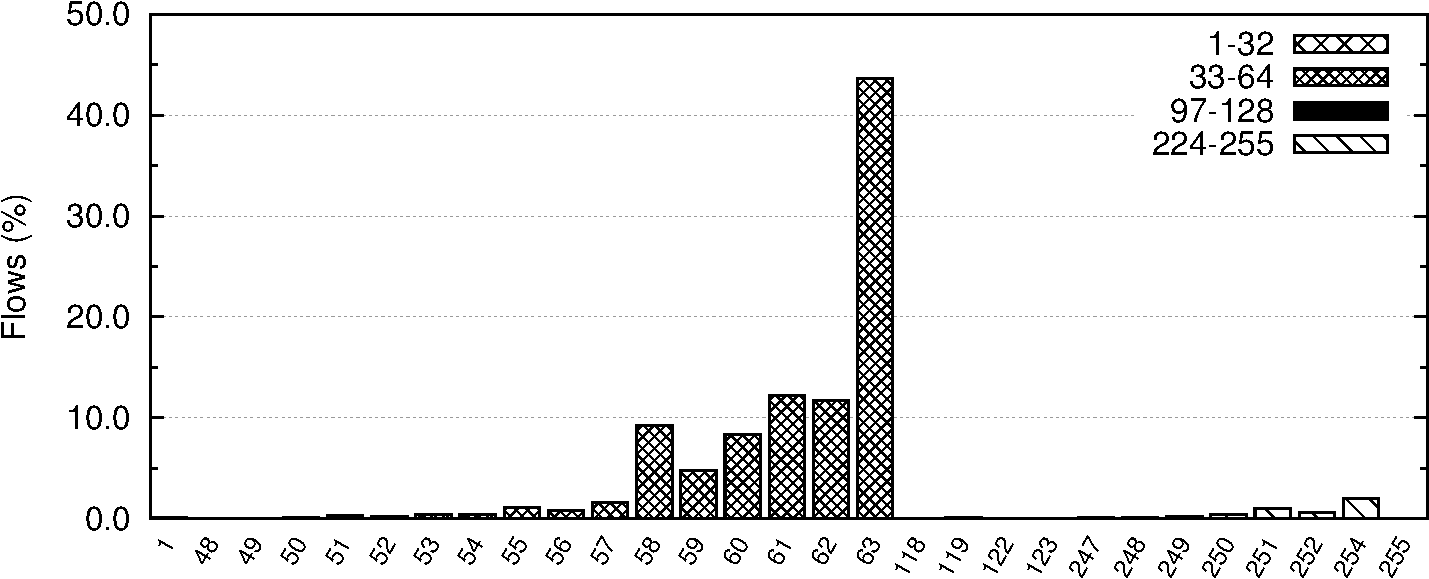
\includegraphics[width=1.00\linewidth]{figures/paper-tunnels/ttl/native-hop}
        \caption{HOP Value Distribution of IPv6 Traffic}
        \label{fig:ipv6-tunnels-ipv6-native-hop}
\end{figure}


\subsubsection{Location of IPv4 and IPv6 Endpoints}
The second characteristic that we evaluate is \textit{geolocation aspect} of the IPv4 and IPv6 traffic. We focus on data from Telia link only, which connects the CESNET network to the United States. This highlights the differences in geolocation characteristics better. The statistics are computed separately for the incoming and outgoing lines and are shown in Figure~\ref{fig:ipv6-tunnels-top-ten-geo}. The IPv4 is more symmetric since the country statistics for both directions are similar. This is a normal behavior since most of the requests initiate a response and the routes are also symmetric. The IPv6 have different properties. We discovered that the addresses that cannot be geolocated are mostly link-local addresses (fe80::/10) or local-link multicast addresses (ff02::/16). Such addresses should not be routed at all, which indicates that there are routers with erroneous IPv6 configuration. This misconfiguration also causes the asymmetry of the traffic, as such requests cannot be answered.

\begin{figure}[!tb]
     \begin{subfigure}{\textwidth}
        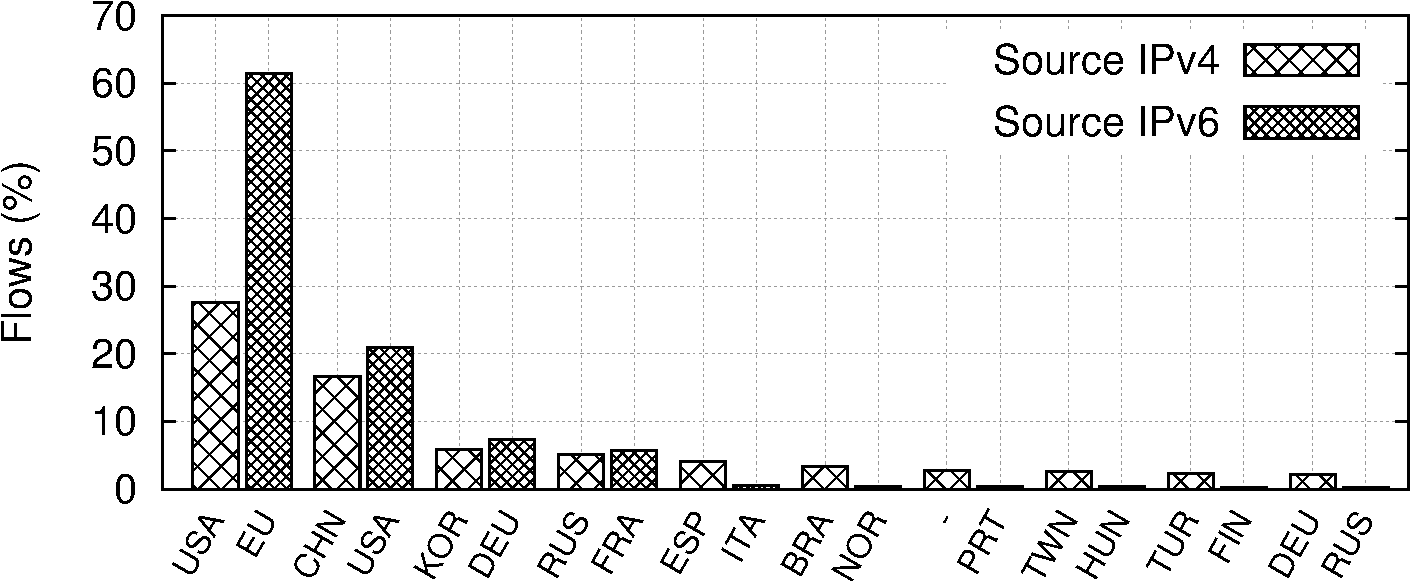
\includegraphics[width=0.97\linewidth]{figures/paper-tunnels/ctry_distribution/ctry_distribution-native-in}
        \caption{Incoming Traffic}
        \label{fig:ipv6-tunnels-geo-native-in}
    \end{subfigure}
    \hfill
    \begin{subfigure}{\textwidth}
        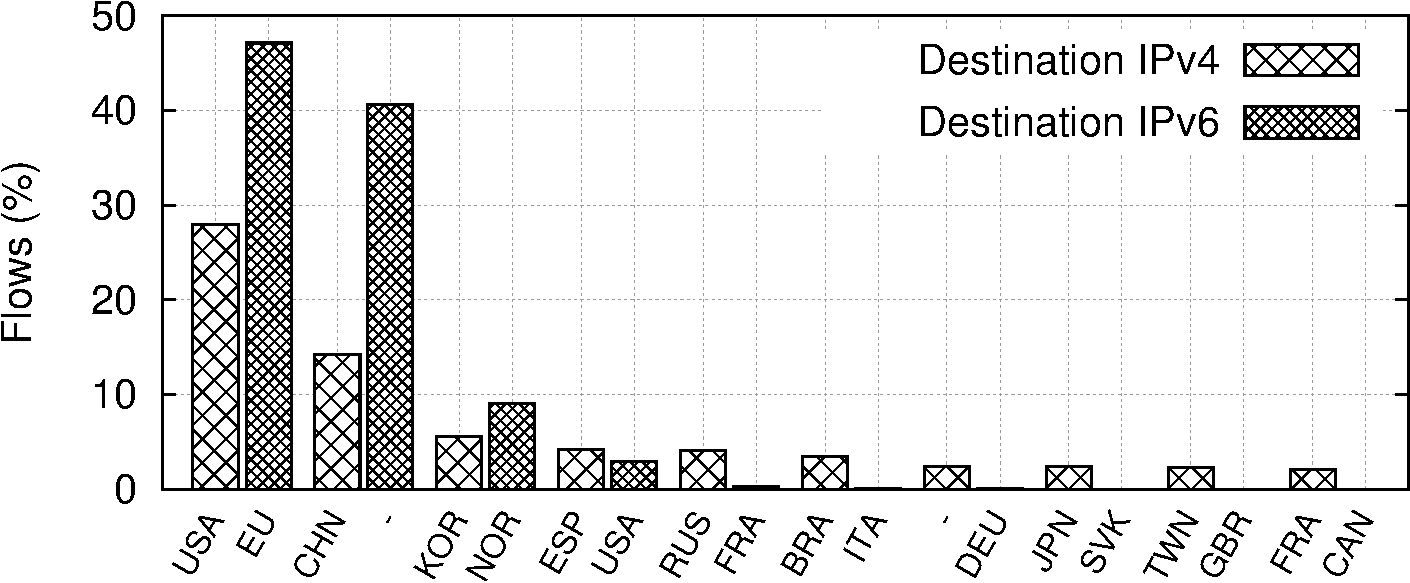
\includegraphics[width=0.97\linewidth]{figures/paper-tunnels/ctry_distribution/ctry_distribution-native-out}
        \caption{Outgoing Traffic}
        \label{fig:ipv6-tunnels-geo-native-out}
    \end{subfigure}
    \caption{Top 10 Country Distribution for Native IPv4, IPv6 and Decapsulated IPv6 Addresses}
    \label{fig:ipv6-tunnels-top-ten-geo}
\end{figure}

\subsection{Duration and Size of Flows}
The third group of characteristics is represented by flow duration, number of packets per flow and packet size (bytes per packet) statistics. For evaluation we employ \textit{empirical complementary distribution function} (CCDF). We use the following formula to compute CCDF values:

\begin{align}
    \bar{F}(x)= P(X>x)=1-\frac{1}{n}\sum^{n}_{i=1}\mathbf{1}\{x_{i}\leq x\}
\end{align}

where $\mathbf{1}\{x_{i}\leq x\}$ is the indicator whether the event $\{x_{i}\leq x\}$ has occurred or not. The CCDF function describes how often the selected variable is above a particular level. From all traces we filtered out four subsets of traffic: TCP or UDP encapsulated traffic (TCP/UDP), all encapsulated traffic (ALL), IPv6 native or decapsulated traffic (IPv6) and IPv4 traffic (IPv4). The subsets were chosen in order to compare the tunneled traffic with other common traffic types. Further, for each of the subsets and each of the characteristics CCDF has been computed. Figure~\ref{fig:ipv6-tunnels-cdf_duration}, \ref{fig:ipv6-tunnels-cdf_packets} and \ref{fig:ipv6-tunnels-cdf_bytes} show the calculated CCDFs.

\begin{figure}[!tb]
     \centering
     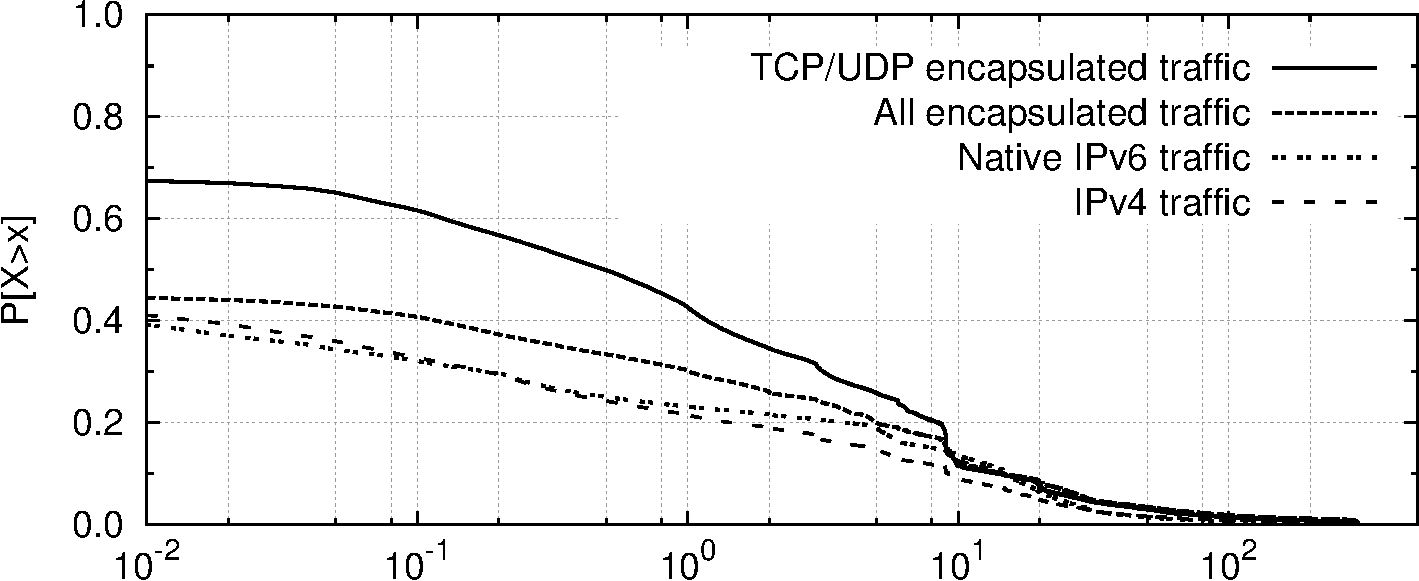
\includegraphics[width=1.00\textwidth]{figures/paper-tunnels/cdf_functions/cdf_duration}
     \caption{CCDF of Flow Duration}
     \label{fig:ipv6-tunnels-cdf_duration}
\end{figure}

\begin{figure}[!tb]
     \centering
     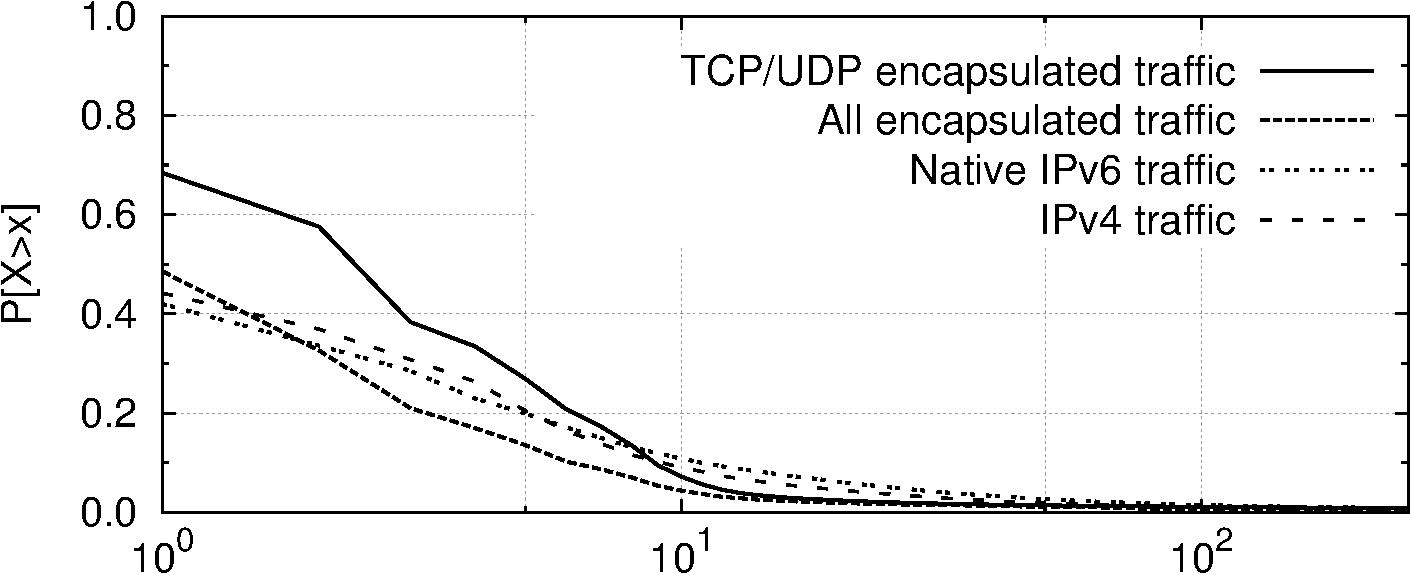
\includegraphics[width=1.00\textwidth]{figures/paper-tunnels/cdf_functions/cdf_packets}
     \caption{CCDF of Packets per Flow}
     \label{fig:ipv6-tunnels-cdf_packets}
\end{figure}

\begin{figure}[!tb]
     \centering
     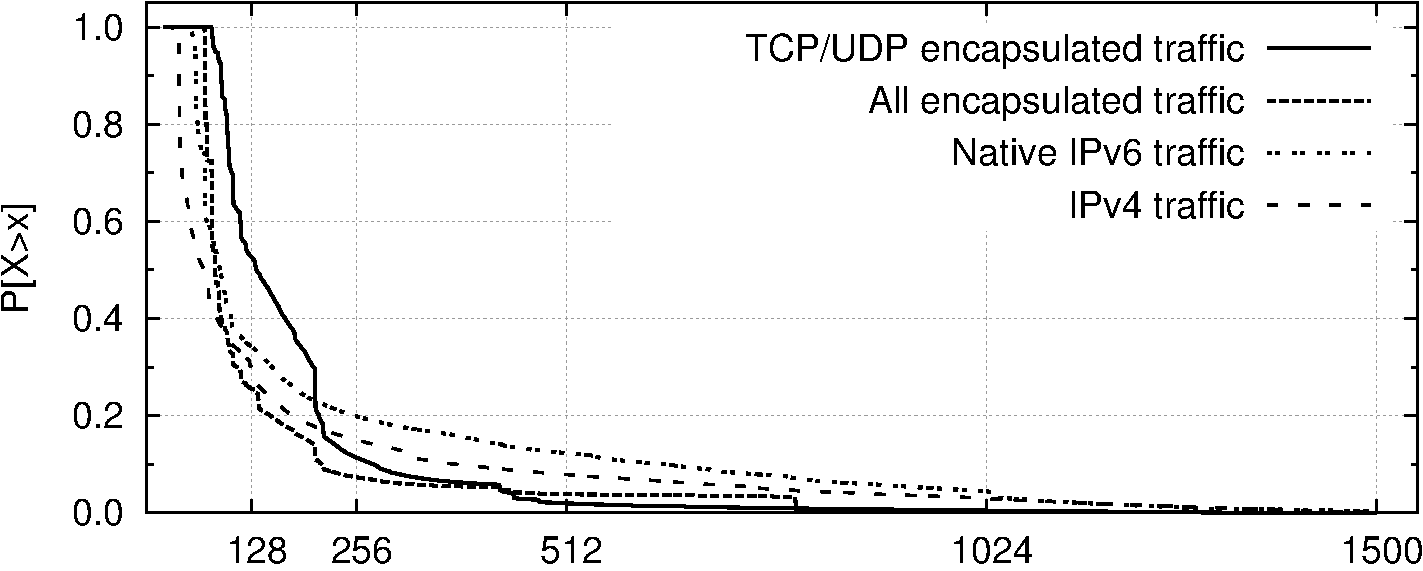
\includegraphics[width=1.00\textwidth]{figures/paper-tunnels/cdf_functions/cdf_bytes}
     \caption{CCDF of Packet Size}
     \label{fig:ipv6-tunnels-cdf_bytes}
\end{figure}

The majority of the flow duration of all subsets (Figure~\ref{fig:ipv6-tunnels-cdf_duration}) accounts for durations shorter than 10 seconds. The flow durations longer than 10 seconds represent only 11\,\% or less. The TCP/UDP contains much fewer short duration flows (TCP/UDP: 32.16\,\% $\leq$ 0.01 sec.; ALL: 54.66\,\%; IPv4: 59.84\,\%) which is explained by the absence of connection-maintaining flows necessary for other subsets. We can observe slightly increased frequencies of the flow duration between 7 and 11 seconds especially at TCP/UDP and ALL subsets. Hence, the tunneled traffic generally contains fewer short duration flows than IPv4 or IPv6 traffic.

The packets per flow distribution (Figure~\ref{fig:ipv6-tunnels-cdf_packets}) suggests that single packet flows form only 31.6\,\% in the case of TCP/UDP, 51.42\,\% in the case of ALL, 57.99\,\% and 55.82\,\% in other cases. We expected tunneled traffic to behave in a similar way as IPv6 traffic. Nevertheless, we can observe a vertical shift between ALL and IPv6 CCDF. This shift is caused by single packet flows and it is caused by DNS traffic to root DNS servers, which uses IPv6 protocol. The slope of CCDF for TCP/UDP and ALL is higher than the slope for other subsets, which states higher frequencies of certain packet counts. In conclusion, the distribution of the packet counts of the tunneled traffic is slightly different from the distribution of the IPv4 and IPv6 traffic.

The last characteristic described by CCDF is packet size (Figure~\ref{fig:ipv6-tunnels-cdf_bytes}). In the case of encapsulated traffic we consider the outer packet size including the encapsulation header. The earlier study of the packet size distribution mentions a significant difference between CCDFs of packet sizes. The authors of~\cite{Ciflikli-2012-Packet} state that the distribution of IPv4 traffic fits a heavy-tailed distribution, whereas IPv6 traffic does not. We expect the tunneled traffic to have similar characteristics as IPv6 traffic, and thus the CCDFs are expected to be similar, too. The Figure~\ref{fig:ipv6-tunnels-cdf_bytes} shows some discrepancies in this hypothesis. The packets larger than 400 bytes in the tunneled traffic represent only 5\,\%, while in the IPv6 the portion is still 15\,\%. Furthermore, packets smaller than 70 bytes are not present in the tunneled traffic, although they account for 26\,\% of IPv6. This is caused by a shift of graph to a higher packet size given by the encapsulation. The IPv4 header is usually 20 bytes long and in case of Teredo there are another 8 bytes for the UDP header. Even taking this shift into account there is still a noticeable drop at size of 200 bytes which is caused by a high share of ICMPv6 and BitTorrent control traffic.


\subsection{IPv6 Tunneled Traffic Analysis} \label{subsec:ipv6-tunnels-inner-traffic-evaluation}

In this section we focus on characteristics of encapsulated IPv6 traffic for which we use the same data set as in Section~\ref{subsec:ipv6-tunnels-outer-traffic-evaluation}. We show HOP limit statistics, detected Teredo servers and geolocation characteristics. We discuss the most used TCP and UDP ports inside the tunnels.

\subsubsection{Distribution of HOP Limits}
Figure~\ref{fig:ipv6-tunnels-tunnels-hop} shows HOP limit distribution for the encapsulated IPv6 traffic. The main difference from the TTL (Figure~\ref{fig:ipv6-tunnels-ipv4-ttl}) and HOP limit (Figure~\ref{fig:ipv6-tunnels-ipv6-native-hop}) statistics is that the values here are distributed with much less entropy. The limits 21, 64, 128 and 255 are achieved and also the most frequent ones. This is caused by the fact that most of the traffic never traversed the IPv6 network and the HOP limit was therefore never decreased. In fact, when the values are lower, we can be reasonably certain that the packets already traversed IPv6 network and are heading towards the IPv4 destination. The value 21 is used for Teredo bubbles by Windows 7 with Service Pack 1 and earlier.The Teredo bubbles are used as a special mechanism for NAT traversal, which is consistent with the fact that most of the clients are behind a NAT. We can see that some packets reach the value of the zero HOP limit, which is a known problem when the HOP limit is set as low as to 21. The value of 255 is used for IPv6 neighbor discovery messages, so that when host receives such packet with HOP limit lower than 255, the packet is considered invalid~\cite{rfc4861}.

\begin{figure}[!tb]
        \centering
        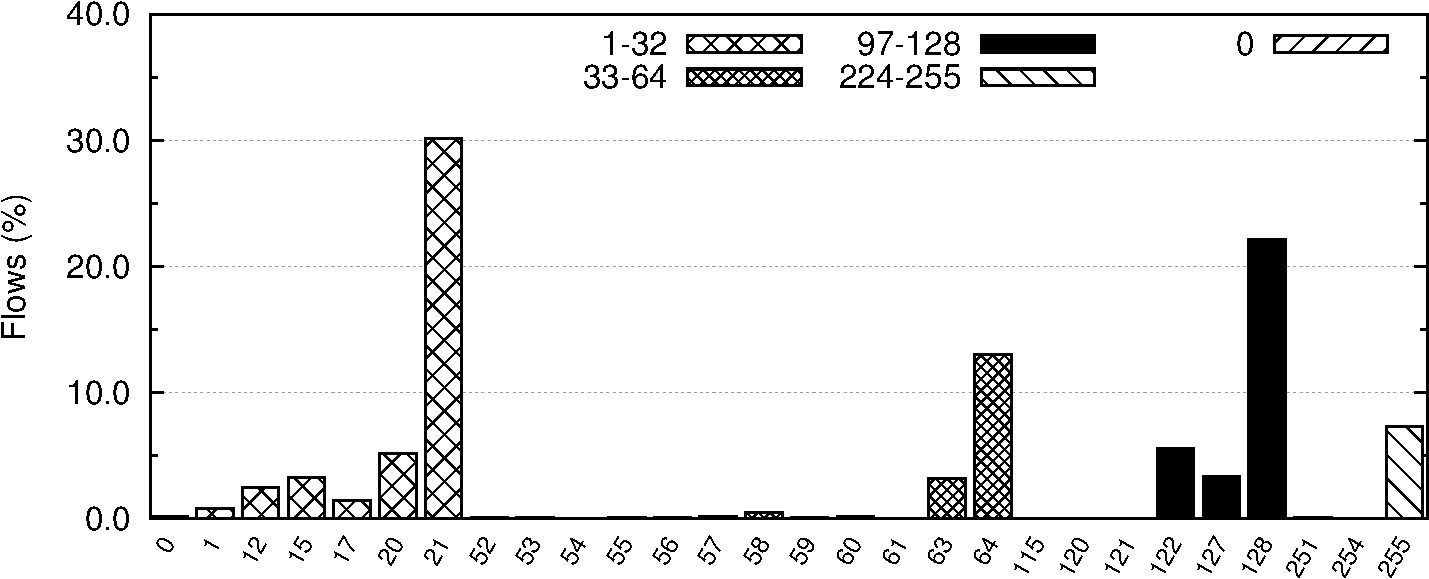
\includegraphics[width=1.00\linewidth]{figures/paper-tunnels/ttl/hop}
        \caption{HOP Value Distribution of Encapsulated IPv6 Traffic}
        \label{fig:ipv6-tunnels-tunnels-hop}
\end{figure}

\subsubsection{Teredo Servers}
There are two ways of detecting Teredo servers. Firstly, we can look at the traffic using UDP protocol on port 3544, which is a well-known Teredo port, and select the addresses that communicate most often. The shortcoming of this approach is that some other services might be using the Teredo port and therefore the results might not be accurate. Since we are able to decapsulate Teredo traffic, we can derive IPv4 addresses of Teredo servers directly from Teredo IPv6 addresses. This way we can even detect Teredo servers that are not communicating directly through our observation points. Table~\ref{tab:ipv6-tunnels-teredo-servers} shows Top 10 servers that were discovered in the encapsulated IPv6 addresses. Using the WHOIS database we confirmed that a majority of servers is operated by Microsoft, which is only to be expected since Teredo is a Microsoft technology. The most of Microsoft Teredo servers we identified are actually IP addresses of "teredo.ipv6.microsoft.com", which is the default Teredo server name configured under Windows. The address $83.170.6.76$ has a hostname indicating that it serves as a Miredo server (Teredo implementation for Linux and BSD). The last address belongs to CZ.NIC (Czech top level domain operator), which is known to promote IPv6 deployment in the Czech Republic and operates local Teredo and 6to4 servers.

Table~\ref{tab:ipv6-tunnels-teredo-servers-3544} shows Teredo servers discovered as the most active on Teredo port 3544. This way we detect only Teredo servers that are establishing connections through our observation points. We can see that most users use Teredo servers in the United States or Great Britain to get IPv6 connectivity. This is known to increase latency of such connections and therefore we would recommend using local servers to Czech users, such as the CZ.NIC servers.

\begin{table}
    \centering
    \begin{subtable}{\textwidth}
        \small
        \centering
        \begin{tabular}{rccc}
            \textbf{Server IP} & \textbf{Ratio} & \textbf{Owner} & \textbf{Country} \\ \toprule 
            65.55.158.118 & 28.33\,\% & Microsoft & US \\
            94.245.121.253 & 27.98\,\% & Microsoft & GB \\
            157.56.149.60 & 26.49\,\% & Microsoft & US \\
            157.56.106.184 & 10.18\,\% & Microsoft & US \\
            94.245.115.184 & 6.41\,\% & Microsoft & GB \\
            83.170.6.76 & 0.04\,\% & B. Schmidt & DE \\
            170.252.100.131 & 0.01\,\% & Accenture & US \\
            94.245.127.72 & 0.01\,\% & Microsoft & GB \\
            94.245.121.251 & 0.01\,\% & Microsoft & GB \\
            217.31.202.10 & 0.01\,\% & CZ.NIC & CZ \\ \bottomrule
        \end{tabular}
        \caption{Based on Teredo IPv6 Addresses}
        \label{tab:ipv6-tunnels-teredo-servers}
    \end{subtable}
    \par\medskip
    \begin{subtable}{\textwidth}
        \small
        \centering
        \begin{tabular}{rccc}
            \textbf{Server IP} & \textbf{Ratio} & \textbf{Owner} & \textbf{Country} \\ \toprule 
            94.245.121.253 & 43.24\,\% & Microsoft & GB \\
            65.55.158.118 & 18.91\,\% & Microsoft & US \\
            157.56.149.60 & 17.86\,\% & Microsoft & US \\
            94.245.115.184 & 10.00\,\% & Microsoft & GB \\
            157.56.106.184 & 6.50\,\% & Microsoft & US \\
            94.245.121.254 & 0.72\,\% & Microsoft & GB \\
            94.245.115.185 & 0.22\,\% & Microsoft & GB \\
            65.55.158.119 & 0.18\,\% & Microsoft & US \\
            83.170.6.76 & 0.18\,\% & B. Schmidt & DE \\
            157.56.149.61 & 0.17\,\% & Microsoft & US \\ \bottomrule
        \end{tabular}
        \caption{Based on UDP Port 3544}
        \label{tab:ipv6-tunnels-teredo-servers-3544}
    \end{subtable}
    \caption{Top 10 Discovered Teredo Servers}
\end{table}

\subsubsection{Location of Tunnel Endpoints}
The geolocation statistics of tunneled traffic are computed for Teredo and 6to4. We use encapsulated IPv6 addresses to determine the countries for each flow. Incoming and outgoing traffic is taken separately just as in Figure~\ref{fig:ipv6-tunnels-top-ten-geo}. The statistics are shown in Figure~\ref{fig:ipv6-tunnels-geo-tun-both}.
The tunneled traffic shows very different geolocation characteristics compared to native and decapsulated IPv6 traffic even though both are from the same link. 
Most of the native and decapsulated IPv6 communication takes place inside the EU, while large portion of tunneled traffic communication is performed with the USA and Russia. 

\begin{figure}[!tb]
    \begin{subfigure}{\textwidth}
        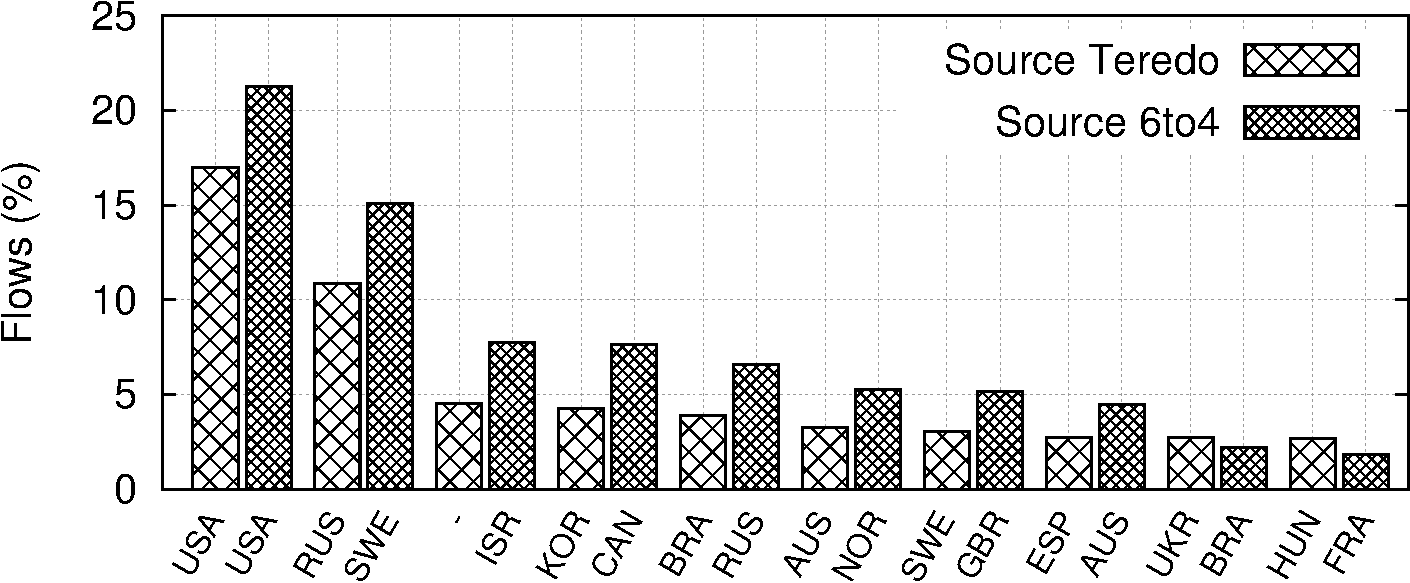
\includegraphics[width=0.97\linewidth]{figures/paper-tunnels/ctry_distribution/ctry_distribution-tun-in}
        \caption{Incoming Traffic}
        \label{fig:ipv6-tunnels-geo-tun-in}
    \end{subfigure}
    \begin{subfigure}{\textwidth}
        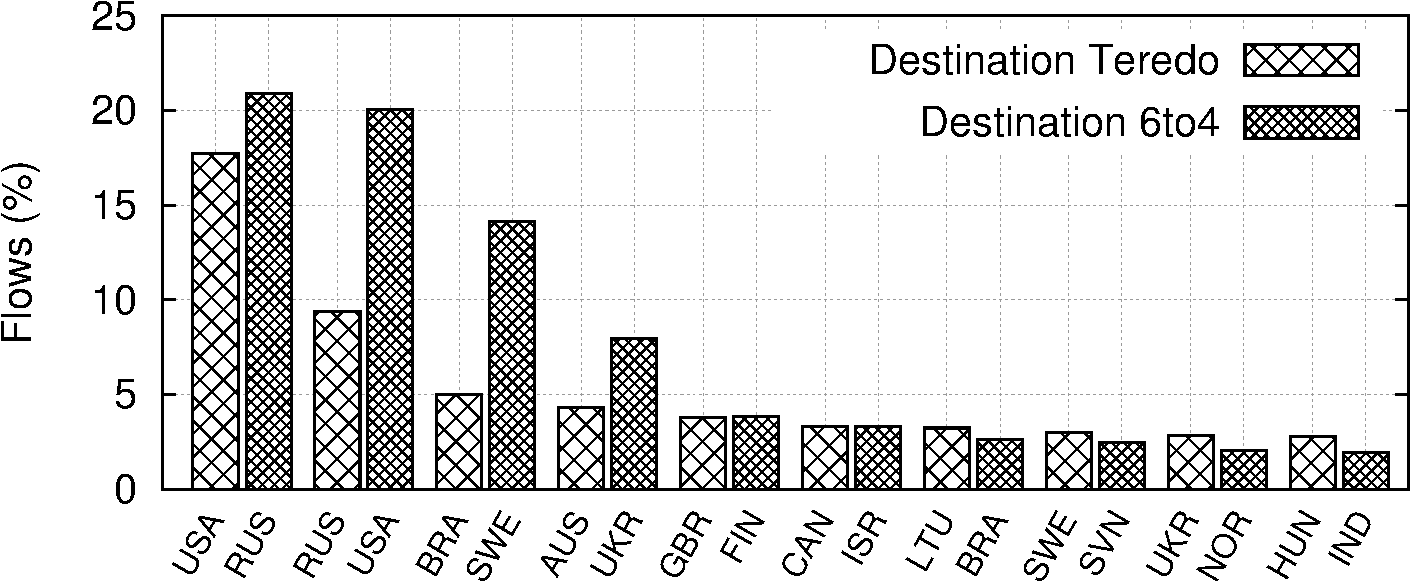
\includegraphics[width=0.97\linewidth]{figures/paper-tunnels/ctry_distribution/ctry_distribution-tun-out}
        \caption{Outgoing Traffic}
        \label{fig:ipv6-tunnels-eo-tun-out}
    \end{subfigure}
    \caption{Top 10 Country Distribution for Encapsulated IPv6 Addresses}
    \label{fig:ipv6-tunnels-geo-tun-both}
\end{figure}

To identify applications that are using IPv6 connection provided by transition mechanisms, we created a list of the most used encapsulated TCP and UDP ports. We observed several ports that can be found both in the source and destination port Top 10. The source and destination ports Top 10 represent 32.0\,\% and 40.5\,\% of the traffic respectively. The well-known ports are - \emph{HTTP - 80} (0.85\,\% of traffic as source port, 5.61\,\% as destination port), \emph{HTTPS - 443} (0.58\,\% and 1.48\,\%) and \emph{DNS - 53} (1.49\,\% and 1.48\,\%). Among the most frequent ports are ports 49001 (15.96\,\% and 9.91\,\%) and 51413 (10.12\,\% and 16.07\,\%) which are used by BitTorrent clients (namely Vuze
and Transmission). We discovered that these ports are heavily used within the 6to4 tunnel as mentioned in Section \ref{subsec:ipv6-tunnels-outer-traffic-evaluation}.

\subsection{Evaluation of IPv6 Adoption} \label{subsec:ipv6-tunnels-evaluation-of-ipv6}

In this section we describe the deployment of the IPv6 protocol with respect to tunneled traffic. The overall statistics of IPv6 and tunneled traffic are mentioned. We provide a historical comparison to our previous measurement~\cite{Elich-2011-Monitoring}. 

The network activity shows the correlation with human activity. Both IPv6 and tunneled traffic are considerably smaller during the weekend than during week days. As for the IPv6 traffic, the increase of traffic volume starts at 6 AM, reaches the peak around 11 AM and holds the high level till 4 PM. Then the traffic steadily decreases and reaches the minimum at 3 AM the next day. The tunneled traffic shows slow increase that starts at 6 AM and peaks around 6 PM. The decrease begins at 10 PM and reaches the minimum at 5 AM the next day. The possible cause of this shift from the IPv6 diurnal pattern is the fact that the tunneled traffic is widely made by BitTorrent clients.

We measured the tunneled traffic back in 2010 on three CESNET border links to SANET, PIONIER and NIX. We found that the tunneled IPv6 was responsible for 1.5\,\% of total flows, which is the same share as we measured today. But the relative amount of bytes transferred has almost doubled from 0.66\,\% to 1.28\,\% of total bytes today. The share of the native and decapsulated IPv6 was only 0.10\,\% (0.21\,\% of bytes) compared to 3.39\,\% (4.42\,\% of bytes) today. The known services by port (HTTP, HTTPS and DNS) had a share less than 1\,\% of total flows. Today's share of these services is significantly higher (see Section~\ref{subsec:ipv6-tunnels-inner-traffic-evaluation}). The measurements show that the overall usage of both tunneling IPv6 transition mechanisms and native IPv6 has been raising.

We distinguish between the encapsulated and decapsulated tunneled traffic, as mentioned in Section~\ref{subsec:ipv6-tunnel-traffic}. The decapsulated tunneled traffic is included in the measured IPv6 traffic. When we filter out the decapsulated Teredo and 6to4 traffic, they account together for 5.91\,\% of the measured IPv6 traffic. Teredo traffic takes part of 83.13\,\% of the decapsulated tunneled traffic and 6to4 16.87\,\%. Hence we should not consider all measured IPv6 traffic as native IPv6 traffic.

The main contributor to tunneled traffic was Teredo with an occurrence of nearly 89\,\% followed by 6to4 with over 11\,\%, therefore the relative amount of 6to4 traffic has increased. We then detected the use of 13 Teredo servers compared to 53 today. %The complete list of the detected servers can be downloaded at the project web page~\cite{web}. 

\subsection{Conclusion} \label{subsec:ipv6-tunnels-conclusion}

In this section we have taken a detailed look at the IPv6 transition mechanisms. We have provided an improved version of our tool for investigating IPv6 tunneled traffic. Considerable progress has been made with regard to understanding tunneled traffic behavior, especially concerning Teredo and 6to4 traffic. The results of this section suggest that encapsulated traffic differs from IPv4 and IPv6 in several characteristics including TTL values, geolocation aspect and flow duration. Moreover, we have provided the list of Teredo servers and described the evolution of IPv6 adoption.


%%%%%%%%%%%%%%%%%%%%%%%%%%%%%%%%%%%%%%%%%%%%%%%%%%%%%%%%%%%%%%%%%%%%%%%%%%%%%%%%%%%%%%%%%%%%%%%%%%%

\section{Large-Scale Geolocation for NetFlow}\label{sec:analysis-geolocation}

Geolocation of network traffic is the process of identifying the geographical location of hosts, by means of their IP addresses. The addition of this information to network traffic is useful for many activities, such as business advertisements, fraud detection and access control. Several types of geolocation can be identified. Active geolocation estimates the location of hosts mostly based on delay measurements~\cite{Katz-Bassett-2006-Towards, Eriksson-2010-Learning}. This results in a high accuracy, but comes at the expense of lack of scalability, and high measurement overhead~\cite{Poese-2011-IP}. On the other hand, passive geolocation relies on static datasets, such as databases, containing the geolocation information per IP address block. Online databases, such as geoPlugin~\cite{--geoPlugin}, can be accessed easily from Web applications and often apply rate or request limiting. This makes them less suitable for bulk geolocation and high-interaction applications. Offline databases, such as MaxMind GeoLite~\cite{MaxMind--GeoLite} and IP2Location~\cite{IP2Location--IP}, do not have these limitations. Both the fact that databases can become outdated and that the majority of data used by passive geolocation approaches refers only to a few popular countries, impact the accuracy of these approaches~\cite{Poese-2011-IP}.
 
Existing geolocation approaches are designed for on-demand, mostly small-scale purposes, where the geolocation is performed by analysis applications that retrieve the flow data from collectors. However, when geolocation needs to be performed in large, high-speed networks, these approaches are not scalable anymore. The main reason for this is that the dataset to be geolocated is too large for these applications, mainly because multiple flow exporters are typically exporting flow data to a single collector. Also, these applications are often developed for data visualization, rather than bulk processing.

The goal of this section is to demonstrate how flow-based geolocation can be performed in a large-scale fashion. As a first step, we propose a prototype for exporter-based geolocation, which adds geolocation data to flow records before they are sent to a collector. As such, the actual geolocation can be distributed over multiple exporters instead of being deployed on a single collector. Since data analysis is almost always done at a collector or by analysis applications that retrieve data from the collector, we also propose an extension to the state-of-the-art flow collection and analysis tool \textit{NfSen}~\cite{Haag-2011-NfSen} that adds native geolocation support. We define \textit{native geolocation support} as the ability to process geolocated flow data in the same way as non-geolocated flow data with respect to storage, filtering, aggregation and statistics generation. After presenting the two prototypes, we analyze the performance footprint of our approaches on the primary tasks of flow exporters and collectors, and present several use cases that demonstrate the practical applicability of large-scale geolocation.

The remainder of this section is structured as follows. Subsection~\ref{subsec:geo-related_work} provides an overview of related works in the field of flow-based geolocation. The main contribution of this work is described in Subsections~\ref{subsec:geo-exporter_based_geolocation} and~\ref{subsec:geo-collector_based_geolocation}, where we present how we perform large-scale geolocation on flow exporters and collectors, respectively. In Subsection~\ref{subsec:geo-prototype_deployment} we describe the deployment of our prototypes and in Subsection~\ref{subsec:geo-use_cases} we present several use cases, which demonstrate their viability. Finally, we close this section in Subsection~\ref{subsec:geo-conclusions}, where we draw our conclusions.

\begin{figure}[!tb]
    \centering
    \begin{subfigure}[t]{0.5\textwidth}
        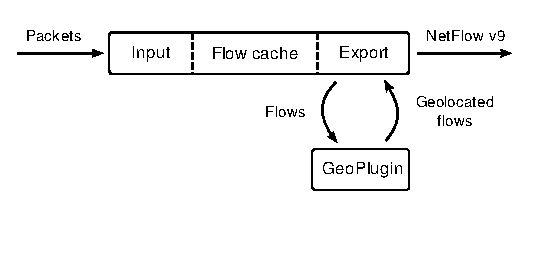
\includegraphics[width=\textwidth]{figures/paper-geolocation/exporter-arch}
        \caption{Exporter-Based Geolocation}
        \label{fig:geo-exporter-arch}
    \end{subfigure}%
    \begin{subfigure}[t]{0.5\textwidth}
        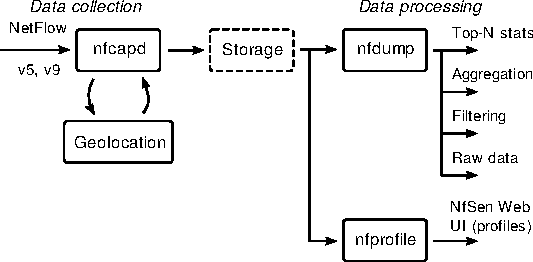
\includegraphics[width=\textwidth] {figures/paper-geolocation/collector-arch}
        \caption{Collector-Based Geolocation}
        \label{fig:geo-collector-arch}
    \end{subfigure}
    \caption{Prototype Architectures for Large-Scale Geolocation.}
    \label{fig:geo-architecture}
\end{figure}

\subsection{Related Work} \label{subsec:geo-related_work}

Due to the increasing number of application areas for geolocation, many related works have been developed in the past. Closest to our work is \textit{nProbe}, a NetFlow/IPFIX probe for exporting NetFlow data to a flow collector~\cite{--nProbe}. This flow exporter uses MaxMind GeoLite~\cite{MaxMind--GeoLite} for the conversion of IP addresses to geographical locations and AS numbers. The fact that geolocation by \textit{nProbe} is exporter-based makes it scalable for use in large-scale networks. However, by storing the geolocation information in special fields, software support by collectors and applications is required to access this data. Geolocation by \textit{nProbe} is therefore not transparent to any flow collector, which makes this approach different from our work.

Other related works, such as \textit{SiLK}~\cite{CERTNSAT--SiLK}, \textit{ntop}~\cite{--ntop} and \textit{Argus}~\cite{QoSient--ARGUS}, are collector-based. \textit{SiLK} and \textit{ntop} add geolocation information to flow data both in an on-demand fashion and as a post-processing step. As such, geolocation information is used purely for visualization and native geolocation is not supported. \textit{Argus} is more advanced, since it creates an extended dataset from the NetFlow data, in which it can also store geolocation data. As such, full geolocation support is provided as long as the geolocation data has been added as a post-processing step to the dataset before.

Besides exporter- and collector-based geolocation approaches, dedicated analysis applications have also been developed. These applications retrieve flow data from flow collectors and subsequently perform the geolocation. \textit{SURFmap}~\cite{Hofstede--SURFmap, Hofstede-2009-SURFmap}, a plugin for the flow collector \textit{NfSen}, uses geolocation to visualize network traffic on a map using the Google Maps API. Due to a dependency on the Google Maps Geocoder for translating location names to coordinates, only a limited number of queries can be executed per day. A \textit{geofilter} has been included since version 2.3, which aims to filter flow data based on country, region or city keywords as a post-processing step. The specification of this \textit{geofilter} is one of the core elements of our collector-based geolocation prototype. Another application is \textit{HAPviewer}~\cite{Blatter-2011-Extending}, which is able to provide flow-level statistics per country of communication partners. Both \textit{SURFmap} and \textit{HAPviewer} perform geolocation on-demand and do not provide native geolocation support.

\begin{figure*}[!tb]
    \centering
    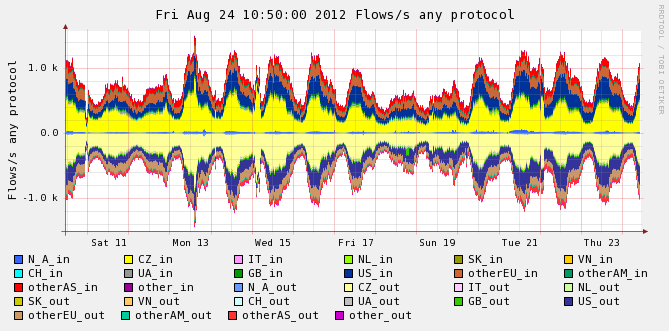
\includegraphics[width=\textwidth]{figures/paper-geolocation/nfgeodump.png}
    \caption{Screenshot of Collector-Based Geolocation Prototype.}
    \label{fig:geo-nfgeodump_screenshot}
\end{figure*}

\subsection{Exporter-Based Geolocation} \label{subsec:geo-exporter_based_geolocation}

Flow exporters can perform more tasks than only flow export nowadays, due to their increasing performance. We propose a prototype for exporter-based geolocation, which adds geolocation data to flow records in a way that is transparent to standard flow collectors. This means that the geolocation data can be accessed by any standards-compliant collector. Usually, multiple flow exporters send their data to a single flow collector. An exporter-based approach therefore aims to distribute the geolocation process over multiple devices. This improves the overall scalability in large networks and reduces the performance footprint on flow collectors.

Our exporter-based geolocation prototype has been developed as a plugin for the FlowMon~\cite{FlowmonNetworks--Flowmon} platform. Plugins can be used to alter flow creation, processing, filtering and export. The architecture of FlowMon is shown in Fig.~\ref{fig:geo-exporter-arch}. Packets on the line are received by \textit{input} plugins that store newly created flow records in the \textit{flow cache}. As soon as a record in the cache has been expired (\textit{e.g.} due to a timeout), it is removed from the cache, after which the \textit{export} plugin takes care of placing it in NetFlow packets. Our geolocation plugin is depicted as \textit{GeoPlugin}, which is executed by the \textit{export} plugin just before the record is exported. \textit{GeoPlugin} will do the actual geolocation and add the resulting data to the flow record.

To make sure that our exporter-based geolocation is transparent to any flow collector, NetFlow v9 has been chosen as the export protocol. It provides a fixed set of fields that can be used to store information about a flow. To add country-level information to flow records, we either have to use reserved (vendor proprietary) fields, or reuse some of the existing fields. Only country-level geolocation information is considered in this work, due to the poor accuracy of geolocation databases with respect to region- and especially city-level geolocation data~\cite{Poese-2011-IP}. NetFlow's reserved fields are typically not supported by collectors, which leaves the reuse of existing fields as the only option to ensure transparency, compatibility and early deployment. Since the \textit{SRC\_AS} and \textit{DST\_AS} fields are rarely used in typical flow monitoring setups (due to the lack of BGP data integration), we use these fields for storing the source and destination countries of IP addresses in flow records. After retrieving the geolocation data from the MaxMind GeoLite database, the resulting country-code is converted to a numerical value and stored in these fields. When flow collectors and analysis applications need to access the country-level information in the flow records, the \textit{SRC\_AS} and \textit{DST\_AS} fields need to be parsed and the values need to be translated to country codes.

There are many advantages of using the IPFIX protocol for exporting geolocation information. IPFIX is more flexible than NetFlow v9, supports more fields (named \textit{IPFIX Information Elements}) and makes it easier to define enterprise-specific fields. Several fields for adding location information to IPFIX have been proposed already in~\cite{draft-irtf-nmrg-location-ipfix-00}. However, those fields are only used for storing the location of an IPFIX flow exporter and are therefore not suitable for flow geolocation. Besides the flexible definition of fields, genuine IPFIX collectors are able to receive new fields and should be flexible enough to process them. However, no suitable IPFIX collectors were available at the time of writing and reusing NetFlow v9 fields served well for our purposes, even though this approach is highly discouraged. Note that switching to the IPFIX protocols is only a matter of adjusting flow exporter configuration.

\subsection{Collector-Based Geolocation} \label{subsec:geo-collector_based_geolocation}

Flow collectors typically aggregate flow data from multiple flow exporters, which makes them a suitable location to perform data analysis. \textit{NfSen} is a popular collector and analysis tool, used by many network administrators in large-scale networks where performance and stability are essential. \textit{nfdump}, an analysis tool included in \textit{NfSen} that takes care of the actual data analysis, uses a flat-file database with an extensible format\footnote{The extensible format is supported by \textit{nfdump} since version 1.5.7.} to read flow data. Several extensions have been included before, such as SNMP interfaces, AS numbers, MAC addresses and VLANs. We propose a new extension for storing source and destination country codes (based on ISO 3166-1) for IP addresses in flow records. For the same reason as explained for our exporter-based approach, only country-level information is considered. Besides the database extensions, also support for filtering, aggregating and statistics generation based on the geolocation data need to be added to \textit{nfdump}, to provide native geolocation support.

Besides \textit{nfdump}, \textit{NfSen} includes several other tools that need to be modified to provide native geolocation support in a flow collector. Among them is \textit{nfcapd}, which receives flow data from flow exporters, performs the actual geolocation (using MaxMind GeoLite) and writes the data to the disk. Obviously, \textit{nfcapd} also needs to support the new flat-file database format of \textit{nfdump}. Other modifications need to be made to \textit{nfprofile}, which performs the traffic profiling for \textit{NfSen}. The overall architecture of our collector-based geolocation prototype and the data flow between the various components is shown in Fig.~\ref{fig:geo-collector-arch}.

A screenshot of our prototype is shown in Fig.~\ref{fig:geo-nfgeodump_screenshot}, which demonstrates one aspect of the native geolocation support: The traffic is now automatically profiled by country names. The introduced geolocation support is completely transparent to and compatible with other parts of \textit{NfSen}, and provides near real-time, long-term traffic profiling based on geolocation. No additional tools are required. There are ongoing discussions with Peter Haag, the developer of \textit{NfSen} and \textit{nfdump}, about integration of our geolocation modifications in the main source tree of these tools.

\subsection{Prototype Deployment} \label{subsec:geo-prototype_deployment}

The two previous sections have discussed our approaches to exporter- and collector-based geolocation. Both approaches aim to translate IP addresses to geographical locations in a scalable manner, for deployment in large-scale networks. To validate whether this aim is fulfilled, we have deployed both prototypes on the 10\,Gbps Internet connection of the Masaryk University (CZ), which connects the campus network to the Czech national research and education network CESNET.

The primary tasks of flow exporters and collectors are data export and collection, respectively. Although geolocation adds a useful new dimension to this data, it should never interfere with the primary tasks of these devices. To analyze the performance footprint of our geolocation, we have measured the number of geolocation queries that could be performed per second. MaxMind GeoLite provides four data retrieval types, namely one file system-based (\textit{standard}) and three memory-based (\textit{memory cache}, \textit{check cache} and \textit{MMAP cache}) ones. Besides them, both IPv4 and IPv6 address geolocation have been tested, since they use different databases with different schemas. The measurement\footnote{We have used a machine with the following configuration: Intel Xeon E5410 CPU at 2.33\,GHz, 12\,GB RAM, SATA disk with 7200\,RPM and Linux kernel 2.6.32 (64 bit).} results are shown in Fig~\ref{fig:geo-mm-perf} and reveal a clear performance increase when either \textit{memory cache} or \textit{MMAP cache} is used: Up to $15.7 \cdot 10^7$ IPv4 and $5.4 \cdot 10^7$ IPv6 addresses could be geolocated per second. Since flow records consist of two IP addresses, roughly $7.8 \cdot 10^7$ IPv4 and $2.7 \cdot 10^7$ IPv6 flow records can be geolocated per second. However, geolocation using memory-based retrieval methods is CPU-intensive and consumes up to 100\,\% of the CPU time. The derived numbers for the geolocation performance can therefore never be reached in practice. In a theoretical case where either the flow export or collection process may consume 50\,\% of the CPU time, roughly $3.9 \cdot 10^7$ IPv4 and $1.4 \cdot 10^7$ IPv6 flow records can be geolocated per second. As a result, the performance of exporters and collectors in our deployment setup is not affected in any way, as we have up to $6.0 \cdot 10^3$ flow records per second to process. Neither will it on backbone links of CESNET, where up to $45 \cdot 10^3$ flow records are exported and collected per second.

\begin{figure}[!tb]
    \centering
    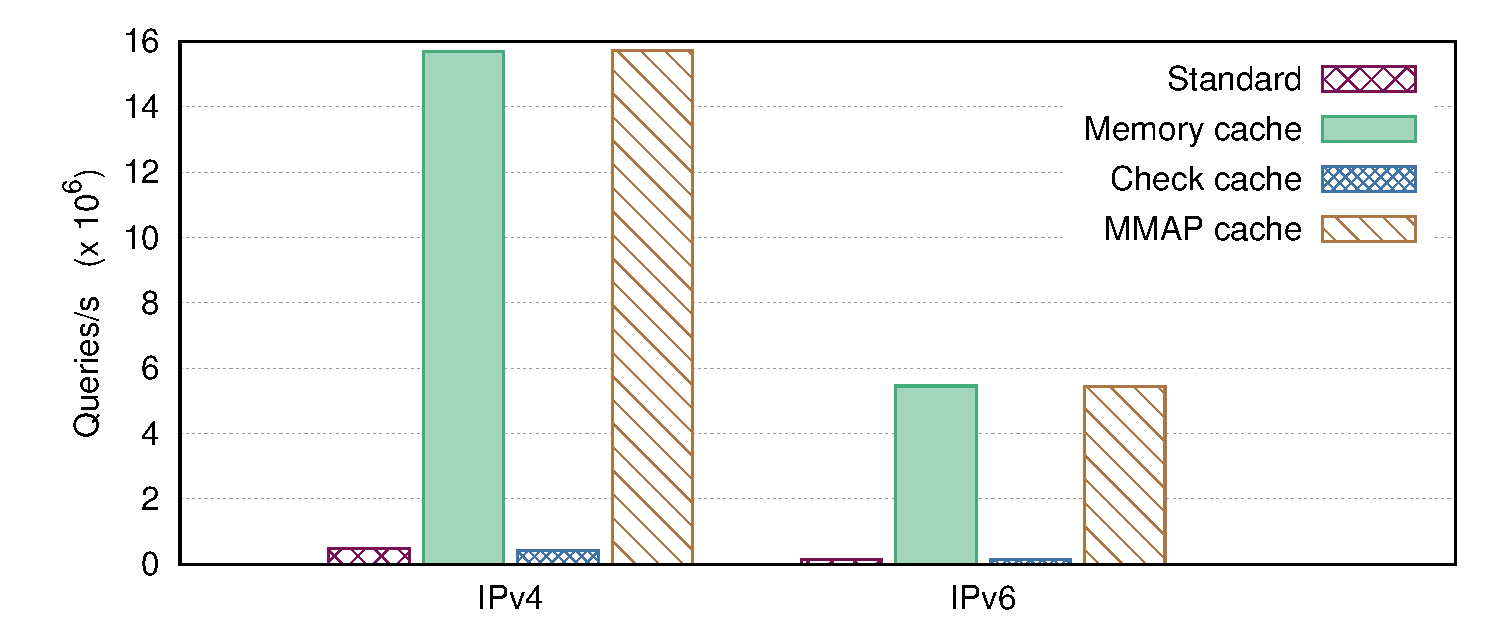
\includegraphics[width=\textwidth]{figures/paper-geolocation/performance/performance}
    \caption{MaxMind GeoLite Country Database Performance}
    \label{fig:geo-mm-perf}
\end{figure}

\begin{figure}[!tb]
    \centering
    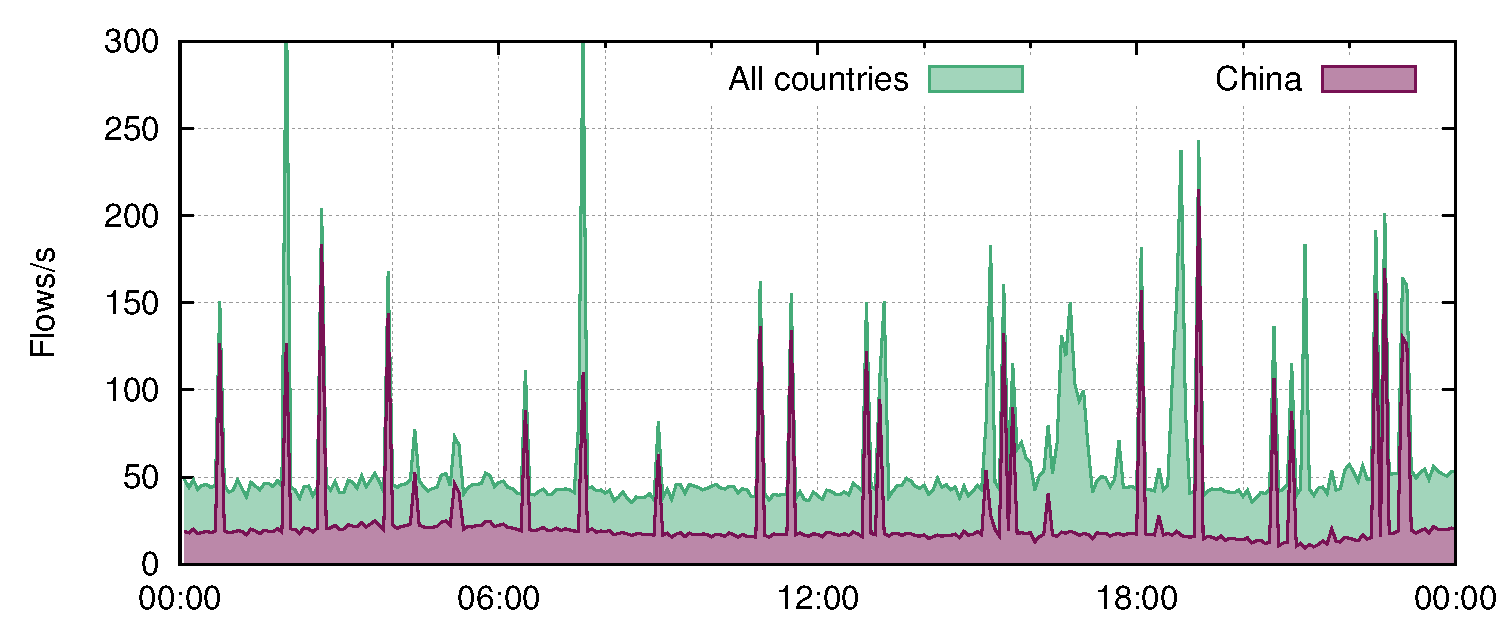
\includegraphics[width=\textwidth]{figures/paper-geolocation/ctry-cn-tw/flows}
    \caption{Incoming TCP SYN-Only Flows}
    \label{fig:geo-tcp-syn}
\end{figure}

\subsection{Use Cases} \label{subsec:geo-use_cases}

In this section, we present analysis results from our collector-based geolocation prototype, organized by two use cases. It is based on the deployment described in Subsection~\ref{subsec:geo-prototype_deployment}. The first use case demonstrates the applicability of our (pre-processed) geolocation approaches for the sake of anomaly detection. The second use case presents week-long traffic profiling at the country-level.

\begin{figure}[!tb]
    \centering
    \begin{subfigure}[t]{\textwidth}
        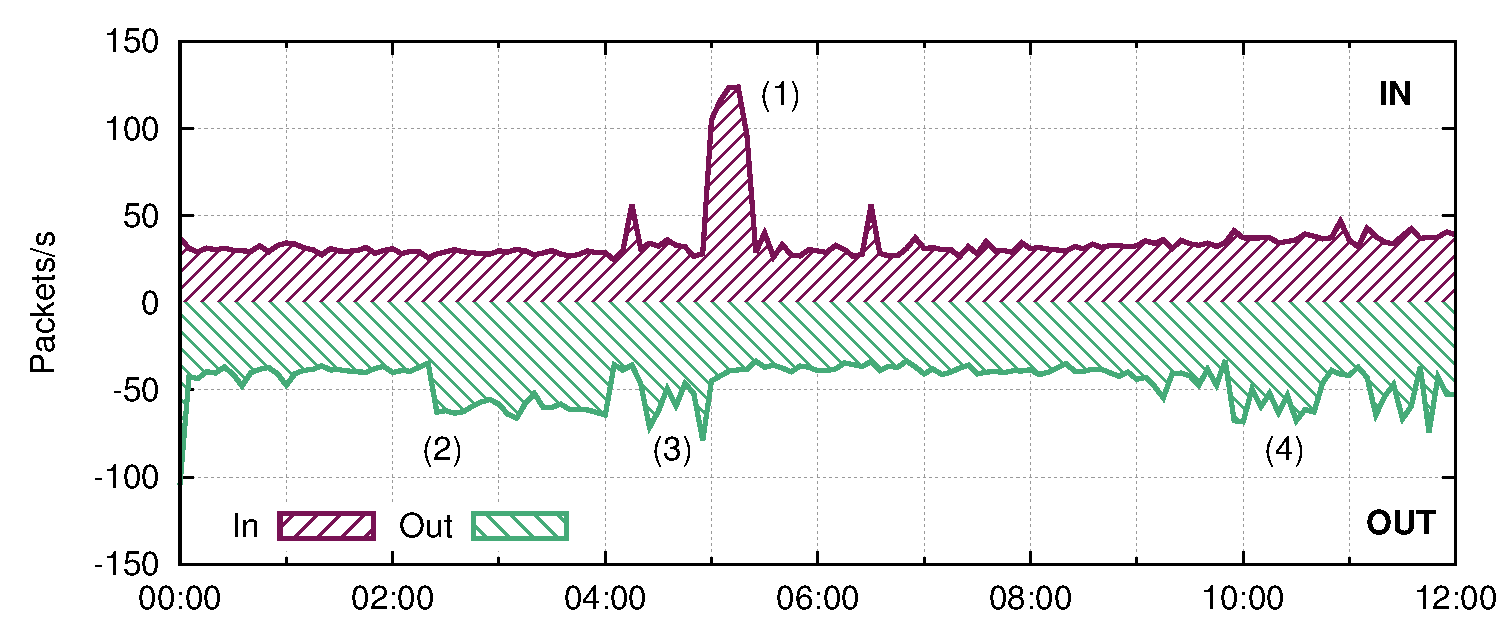
\includegraphics[width=\textwidth]{figures/paper-geolocation/icmp/packets}
        \caption{ICMP}
        \label{fig:geo-icmp-traffic}
    \end{subfigure}%
    \hfill
    \begin{subfigure}[t]{\textwidth}
        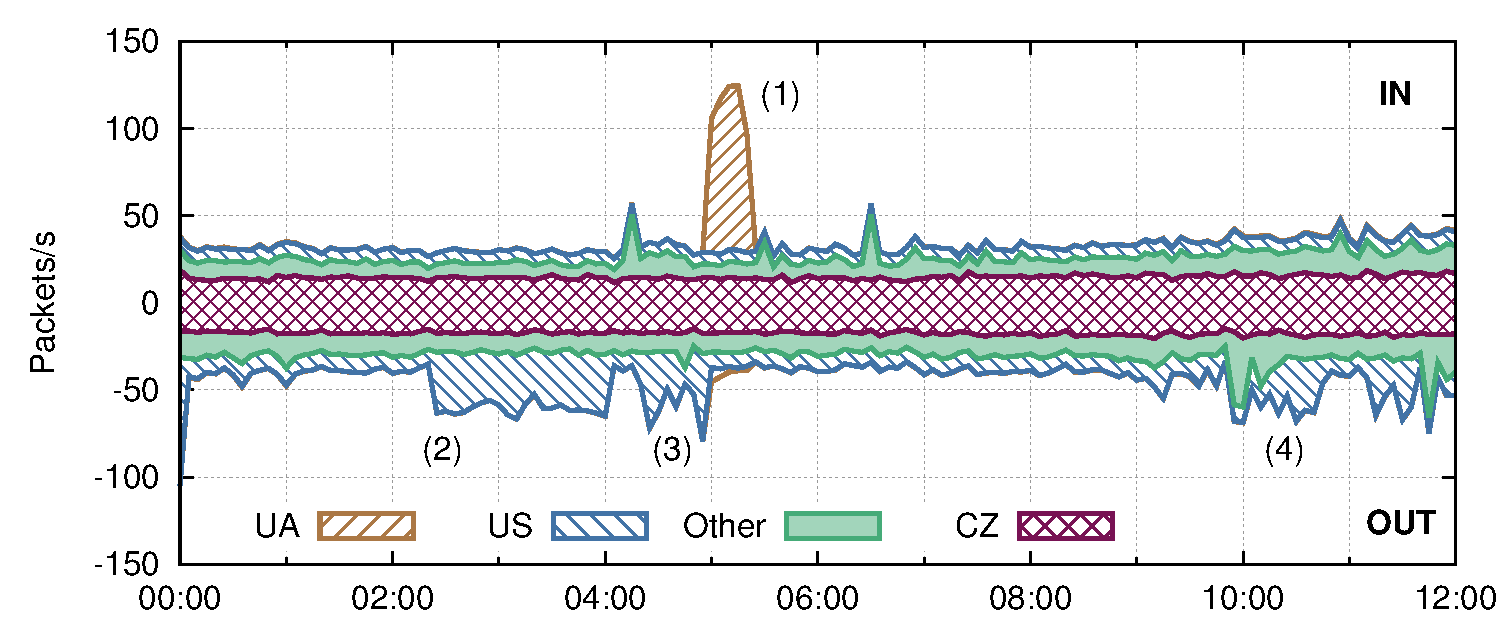
\includegraphics[width=\textwidth]{figures/paper-geolocation/icmp-geo/packets}
        \caption{Geolocated ICMP}
        \label{fig:geo-icmp-geo-traffic}
    \end{subfigure}
    \caption{Geolocated and Non-Geolocated ICMP Traffic}
    \label{fig:geo-icmp}
\end{figure}

\begin{figure}[!tb]
    \centering
    \begin{subfigure}[t]{\textwidth}
        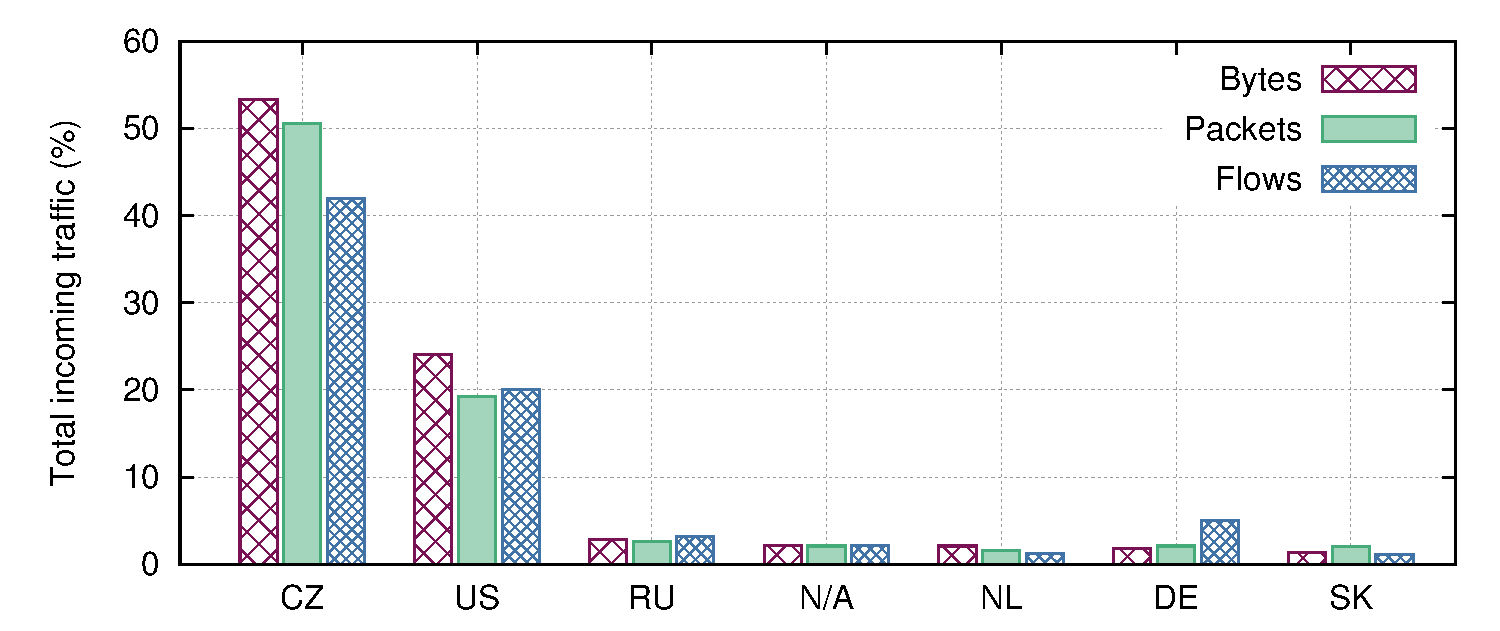
\includegraphics[width=\textwidth]{figures/paper-geolocation/ipv4-ctry-breakdown/ipv4-ctry-breakdown-in}
        \caption{IPv4}
        \label{fig:geo-ipv4-traffic}
    \end{subfigure}%   
    \hfill
    \begin{subfigure}[t]{\textwidth}
        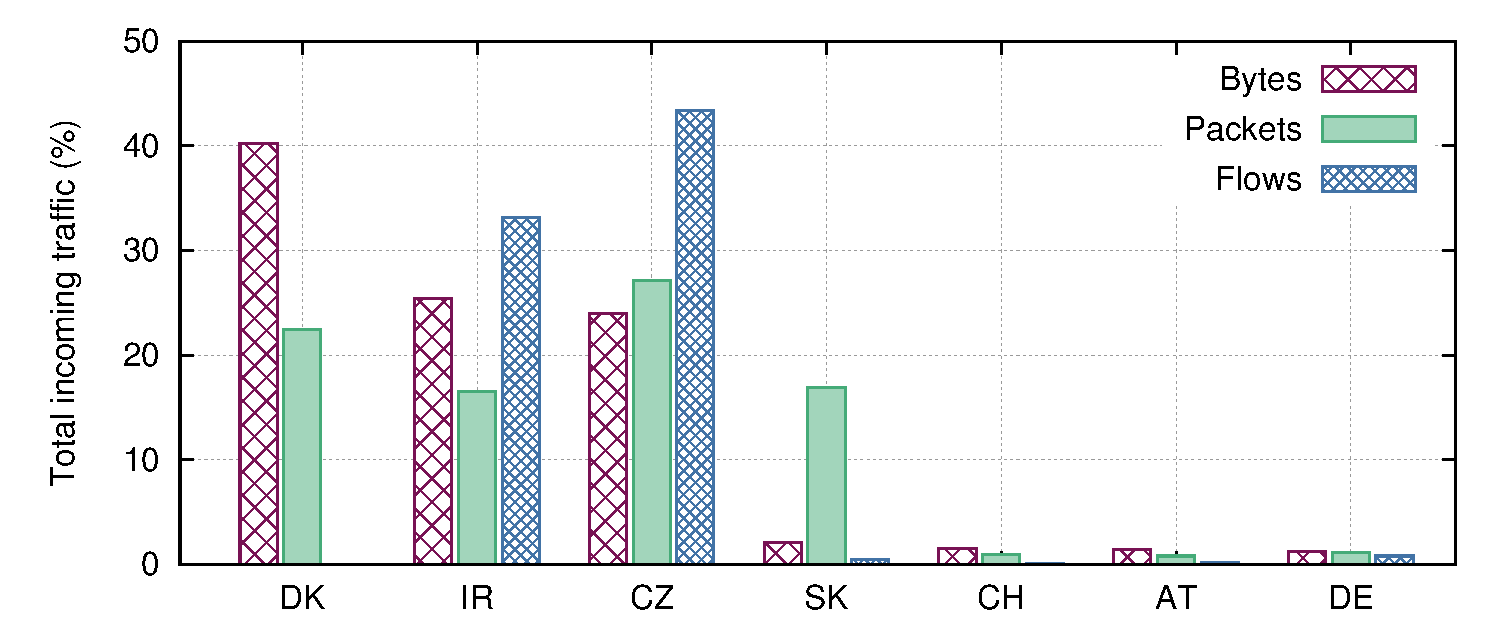
\includegraphics[width=\textwidth]{figures/paper-geolocation/ipv6-ctry-breakdown/ipv6-ctry-breakdown-in}
        \caption{IPv6}
        \label{fig:geo-ipv6-traffic}
    \end{subfigure}
    \caption{Distribution of Incoming Traffic over Countries (1 Week)}
    \label{fig:geo-ip_ctry_breakdown}
\end{figure}

\subsubsection{Anomaly Detection}

It is a difficult task for network administrators to ensure security awareness in the daily barrage of scans, spamming hosts, zero-day attacks and malicious network users, hidden in huge traffic volumes crossing the Internet. When security teams use geolocation for incident analysis, it is usually applied as a post-processing step. In contrast, our approaches perform geolocation as a pre-processing step, which allows to use geolocation data in the detection process, among others.

An example is shown in Fig.~\ref{fig:geo-tcp-syn}, where the number of TCP SYN-only flows\footnote{We denote TCP-flows that consist of a single packet with the SYN-flag set by \textit{TCP SYN-only flows}.} per second during a period of one day is shown. These flows are typically created during the propagation phase of malware. We have identified that more than 40\,\% of them is originating from China. Also, the vast majority of traffic spikes is caused by Chinese connection attempts and only 22\,\% of Chinese TCP traffic completed the TCP-handshake. These findings demonstrate that this particular Chinese traffic is an interesting dataset for anomaly detection and malware analysis. Further investigation has revealed that using geolocation as a pre-processing step for anomaly detection can yield a dataset to be analyzed that is only 40\,\% of its original size in this particular case, resulting in faster and less complex data analysis. This allows to detect anomalies that normally stay below the thresholds of anomaly detection systems. By creating traffic profiles for countries that are known to generate a higher than average amount of malicious traffic, such as China, Russia, Taiwan, Korea and Thailand~\cite{vanPolen-2011-Finding}, we have been able to detect long-term stealth attacks.

Another example that demonstrates the advantages of native geolocation support in a flow collector is shown in Fig.~\ref{fig:geo-icmp}. Fig.~\ref{fig:geo-icmp-traffic} shows an ordinary time-series of ICMP traffic for a period of twelve hours, while Fig.~\ref{fig:geo-icmp-geo-traffic} shows the same traffic but geolocated. Several anomalies - marked by numbers in the figures - can be identified, where the geolocated traffic makes the identification clearer due to the larger relative differences between anomalous and non-anomalous traffic. Peak~1 (incoming traffic) is caused by a Ukrainian host, scanning the complete university network using ICMP ECHO. Replying hosts were later contacted on TCP port 4899. Peaks~2, 3 and 4 (outgoing traffic) are caused by foreign hosts, which are sending spoofed UDP traffic to the university's DNS server to perform an amplification attack. This traffic is blocked by the firewall and ICMP Destination Unreachable is returned to a spoofed source IP address located in the United States.

When network administrators need to find and analyze anomalies using plots as in Fig.~\ref{fig:geo-icmp-traffic}, they can identify the peaks and start to filter the data to determine the hosts involved in an anomaly. However, plots as in Fig.~\ref{fig:geo-icmp-geo-traffic} make these tasks faster and simpler: Since the traffic is already pre-processed by country names, only the datasets related to a specific country need to be analyzed. In the case of Peak~2, for example, this results in a dataset that is only half of its original size.

\subsubsection{Traffic Profiling}

Traffic profiling is the process of analyzing the distribution of services and protocols in a network, such as the number of packets related to Web traffic or the number of flows of a certain type. When geolocation is applied, also statistics related to geographical locations can be generated, such as the number of connections to a certain country. Although this is also possible using existing geolocation approaches based on post-processing, our approach is able to generate these statistics in real-time and for the complete traffic mix. In this subsection, we provide two examples of geolocation-based traffic profiling: IPv4 vs. IPv6 usage statistics and HTTPS profiling.

One method for measuring the world-wide spread of IPv4 and IPv6 deployment is based on counting the number of IPv4- and IPv6-enabled ASNs, respectively. Another method is to measure the percentage of IPv4 and IPv6 traffic per country. For our measurement point in the Czech Republic, the distribution of IPv4 traffic source countries is shown in Fig.~\ref{fig:geo-ipv4-traffic}. The fact that the United States are the source country generating the second most IPv4 traffic is not a surprise, given the fact that US-based social networks (Facebook, Twitter, LinkedIn) and content providers (Akamai, Google, Microsoft) generate a significant portion of the world-wide traffic~\cite{Gehlen-2012-Uncovering}. This is confirmed by both manual inspection of the traffic and Fig.~\ref{fig:geo-https-traffic}, which shows that almost half of the HTTPS traffic, which is commonly used by those services, is going to and coming from the United States. Although the headquarters of these companies are all in the United States, their data is usually hosted closer to the service users, in regional data centers. This is achieved by using geolocation-aware-DNS (GeoDNS), which provides a means for service users to connect to the server that is closest to them from a geographical point of view. By probing the remote hosts in our data sets actively using ICMP ECHO, it is easily verified that the hosts are definitely not located in the United States, due to resulting non-transatlantic round-trip times. This is an example of a major inaccuracy of geolocation databases, which geolocate IP addresses to the companies' headquarters, instead of the real location of hosts.

The distribution of source countries of IPv6 traffic is shown in Fig.~\ref{fig:geo-ipv6-traffic}. Next to Czech Republic, much traffic is received from Denmark and Ireland. Closer analysis has revealed that the Danish traffic is caused by large repository synchronization (using FTP) by two data hosting providers. On the other hand, the Irish traffic is generated mainly by Google and Facebook. Surprisingly enough, this traffic is now geolocated to their real physical location. Google is known to have a large datacenter in Ireland and some Facebook partners, such as Zynga, host their services in the Amazon datacenter in Ireland as well.

\begin{figure}[!tb]
    \centering
    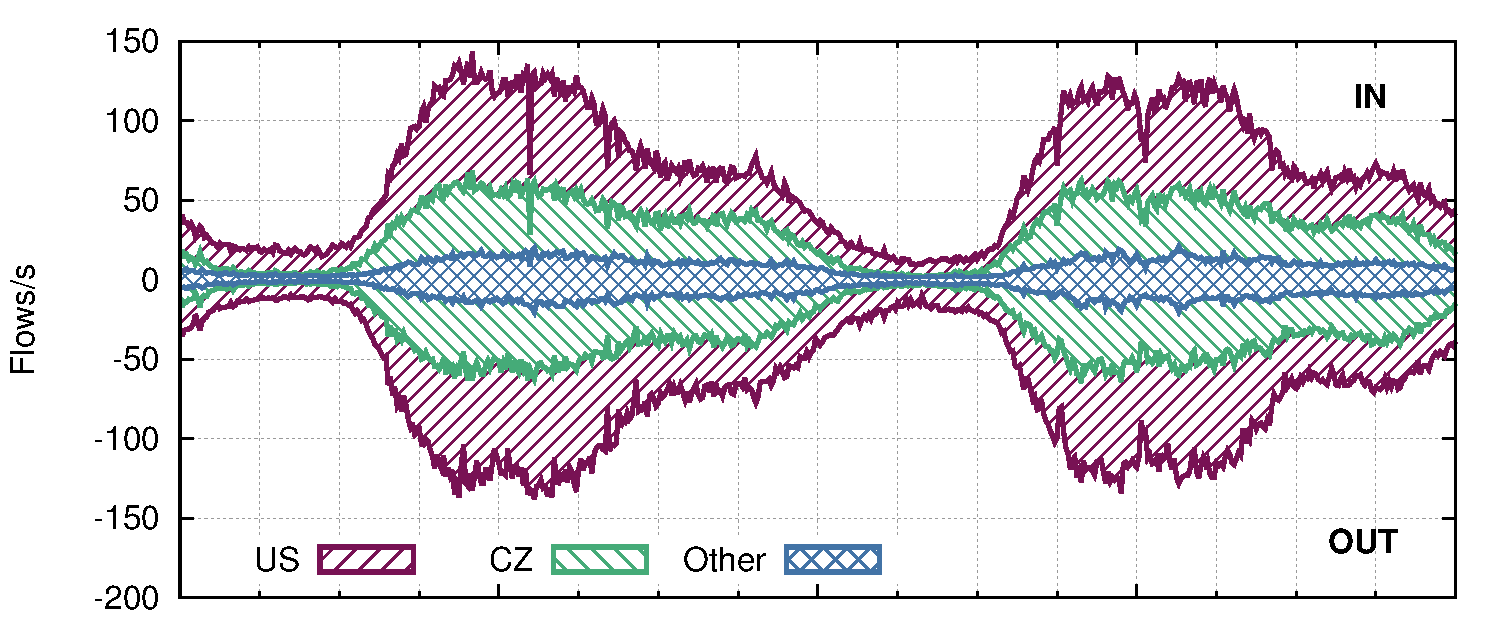
\includegraphics[width=\textwidth]{figures/paper-geolocation/https/flows}
    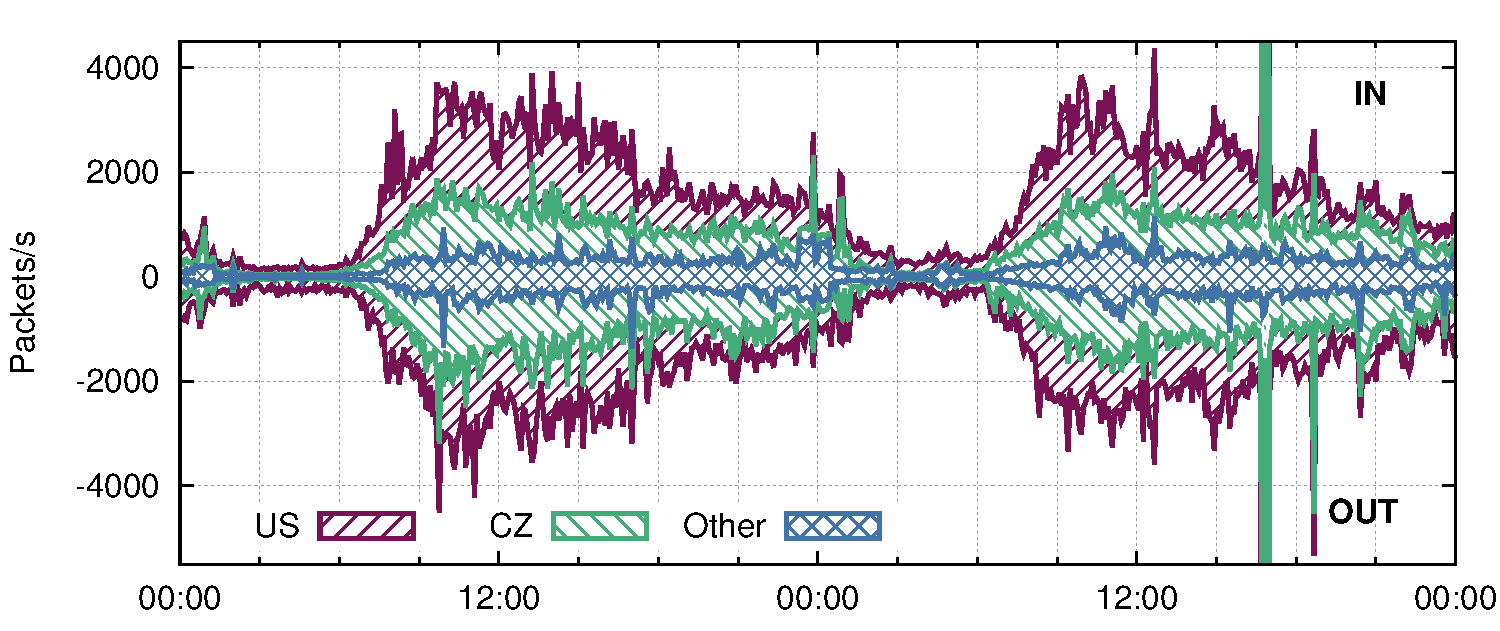
\includegraphics[width=\textwidth]{figures/paper-geolocation/https/packets}
    \caption{Distribution of HTTPS Traffic over Countries}
    \label{fig:geo-https-traffic}
\end{figure}

\subsection{Conclusions} \label{subsec:geo-conclusions}

In this section we presented two prototypes for flow-based geolocation in large-scale networks. Existing approaches to flow-based geolocation have shown not to be suitable for deployment in those networks or to be non-transparent to flow collectors. By integrating geolocation into flow exporters and collectors, we include country-level information in flow data before the actual data analysis takes place. As such, geolocation is performed in real-time as a pre-processing step, instead of the usual post-processing. This allows network administrators to filter, aggregate and generate statistics based on the geolocated data in a continuous fashion. Measurements have shown that the performance footprint of the geolocation process on the actual flow export and collection is negligible.

To demonstrate the applicability of real-time geolocation in large-scale networks, we have shown several examples by means of two use cases. For example, the use case on anomaly detection has shown that geolocation can help reducing the dataset to be analyzed by analysis applications dramatically. If certain countries are expected to generate more malicious traffic than others, traffic from these countries can be pre-filtered. Analysis applications, such as anomaly detection systems, can then analyze the smaller dataset, which results in shorter detection times.

All implementations used in this work are available at \url{http://ics.muni.cz/~celeda/geolocation/}.


%%%%%%%%%%%%%%%%%%%%%%%%%%%%%%%%%%%%%%%%%%%%%%%%%%%%%%%%%%%%%%%%%%%%%%%%%%%%%%%%%%%%%%%%%%%%%%%%%%%


\section{Network Traffic Characterisation Using Flow-Based Statistics}\label{sec:analysis-characterisation}

%% motivation
A lot of research is being performed in the areas of network traffic classification, anomaly detection, and network security in general. Researchers involved in these areas often evaluate their methods using live network traffic. However, performing research on live network traffic includes several caveats. First, repeating experiments on live traffic is infeasible. Second, the traffic has to be thoroughly described, since most methods heavily depend on the properties of the observed traffic. Last but not least, the network traffic's properties can change during the research cycle, which can lead to suboptimal results. Although this work does not directly utilize application flow monitoring, it provides a method of ensuring repeatability of flow monitoring experiments, which is useful both for basic and application flow monitoring.

% repeatability
To be able to repeat the experiments, a packet trace must be captured. Considering the speed and utilisation of current uplinks of the research organisations, hundreds or even thousands of gigabytes of network data would have to be stored. Together with privacy issues, this makes sharing such data sets almost impossible. 

% traffic description & changes
A description of data sets is an important part of any work concerning network traffic. The properties of the traffic highly correlate with the results of any experiments. When the researchers are not able to share their data set, its description should allow other researchers to find a similar data set which would exhibit similar results. Moreover, such a description can be checked for consistency thus ensuring that the results do not unduly fluctuate over time.

%% goals
The goal of this work is to provide a simple method for discerning different types of network traffic. This method allows us to compare network traffic from live networks and even packet traces and determine which traffic samples show similar properties. Finding similar traffic is highly desirable as it allows the independent evaluation of published experiments. Moreover, when applying the method continuously to a specific network, changes in the properties of the network can be not only observed, but also quantified.

Flow-based characteristics~\cite{Hofstede-2014-Flow} are used by our method as they are easier to obtain than packet-based characteristics. Moore et al.~\cite{Moore-2005-Discriminators} list a number of discriminators that can be used for classifying traffic. We select a small subset of discriminators obtained from NetFlow v5~\cite{CiscoSystems-2007-NetFlow} records, that are available from most network devices. Our approach is generic and the set of discriminators can be extended for specific purposes. We show that the chosen discriminators provide enough information to distinguish between various networks.

We analyse the traffic of five campus networks within the Masaryk University. The networks have different properties as they contain a different number of servers, workstations, personal client stations, and portable devices. The networks and the methodology are described in detail so that other researchers can repeat our steps and evaluate their own network traffic.

%% results
We show that it is possible to distinguish between networks based on simple characteristics derived from flow information. Day-night and weekday patterns in the traffic are important phenomena that need to be taken into consideration when deriving characteristics. The characteristics used in this section do not show any significant correlation which indicates that all of them contribute to the description of the network traffic.

%% paper structure
The rest of the section is structured as follows. Related work is surveyed in Subsection~\ref{subsec:characterization-related_work}. We describe the methodology for characterising network traffic in Subsection~\ref{subsec:characterization-methodology}. Results of applying the proposed method on several different networks are shown in Subsection~\ref{subsec:characterization-results}. The section is concluded in Subsection~\ref{subsec:characterization-conclusions}.


\subsection{Related Work} \label{subsec:characterization-related_work}

Statistical properties of Ethernet traffic were studied by Leland et al.~\cite{Leland-1993-Self}. They discovered that the traffic is statistically self-similar, which was later confirmed by several studies~\cite{Crovella-1997-Self, Paxson-1995-Wide}. These studies also showed that detailed characteristics, such as packet inter-arrival times, show large deviations and burstiness. Our study makes use of traffic flow properties which are aggregated over the whole network traffic and therefore much more stable.

Fraleigh et al.~\cite{Fraleigh-2003-Packet} performed packet-level traffic measurement on the Sprint IP backbone. They showed that the measurement interval affects peaks in packet rate and bit rate. Using flow-based analysis makes it possible to normalise the data. Otherwise, it would be more difficult to compare the results from different networks. The authors also showed that different networks have different week and day-night patterns, as well as traffic types and packet size distribution. There was also a discrepancy between flows per second and bits per second for different networks. The authors argued that the network properties depend on the customer type of the link and its location.

Fomenkov et al.~\cite{Fomenkov-2004-Longitudinal} studied network traffic behaviour on long-term data samples. The samples were captured from different networks, one to eight times a day, once per month for 60 to 120 seconds. Only packet headers were stored. The authors used packet, byte and flow rates as well as a number of \mbox{source-destination} IP~addresses to describe long term changes in Internet traffic characteristics. The burstiness of the traffic in combination with short measurement intervals impeded the day-night and weekday patterns. Even the expected long term growth of the traffic was not observed. This advocates using longer measurement intervals in our own work. Despite the intricate nature of the samples used, the authors reported that the average packet length increases with traffic growth. They also observed differences in the composition of traffic transport protocol usage between different networks.

Report of traffic properties measured on a single backbone network link was given by John and Tafvelin in~\cite{John-2007-Analysis}. They collected 148 traces of 20 minutes duration in a single month. The report focused on IP and TCP protocol usage, namely the distributions of IP transport protocols, IP protocol properties, IP and TCP options and flags. Authors also confirmed that the packet size distribution became bimodal as reported by some of the previous researches. A DoS attack was discovered in the collected sample, which caused an anomaly in the number of UDP packets in one of the samples. The report implies that knowing the composition of network traffic is important for the research of anomaly detection and network security.

Benson et al.~\cite{Benson-2010-Network} described traffic characteristics of data centres. They performed a top-down analysis of ten data centres identifying applications used and their communication patterns. The authors observed flow-level and packet-level communication characteristics such as active flows per interval, the distribution of flow sizes and lengths, packet sizes and packet inter-arrival times. They noticed day-night and weekly patterns in the communication and that there is a difference between core and edge links as well as some of the data centres. Their analysis supports our belief that it should be possible to differentiate between network links based on traffic characteristics.

A characterisation of ISP traffic was performed by García-Dorado et al.~\cite{Garcia-Dorado-2012-Characterization}. The authors attempted to provide accurate, extensive, and quantitative measurements of application usage, bandwidth utilisation, and user preferences. They compared customers of different networks and access technologies for long periods of time. Unlike previous findings the daily patterns are reported to be quite invariant, although the weekdays were different from weekends in a campus network. Application traffic shares differed significantly between the individual networks. Moreover, notable changes were observed on the same link during the measurement period. This supports our assumption that measurements on live networks should be well documented and validated.

All of the above-cited works focus on describing the properties and characteristics of network traffic. The key difference to our work is that we identify characteristics that vary between the networks and show that they can be used to differentiate and describe the networks in a uniform manner.

\subsection{Methodology} \label{subsec:characterization-methodology}

To be able to describe network traffic and find key properties that allow us to discern different networks, we collected data from several different parts of our campus network. Understanding the purpose of each network is imperative for the correct interpretation of the data collected, therefore we describe the networks used for collecting the data in detail. This section describes the processes and tools used to collect the data and the collected data itself. 

\subsubsection{A Description of the Networks}

We continually collect data from individual networks in our campus. We chose five networks that are very different by their nature and utilisation. For each network we selected two months of data, January and March. The networks are expected to exhibit different characteristics between the two months, since there is an exam period at Masaryk University in January and March is a standard midterm month. A summary of networks and the collected data is presented in Table~\ref{tab:characterization-measured-networks}.

\begin{table}[!t]
        \centering
%         \small
        \renewcommand{\arraystretch}{1.1}
        \begin{tabular}{|l|r|r|r|} \hline
            \textbf{Network} & \textbf{Packets} & \textbf{Bytes} & \textbf{Flows} \\ \hline
            Faculty of Informatics & 227.1\,G & 236.4\,T & 3.6\,G \\ \hline
            Institute of Computer Science & 107.3\,G & 106.2\,T & 0.7\,G \\ \hline
            University Campus Bohunice & 449.8\,G & 473.9\,T & 4.1\,G \\ \hline
            Virtual Switching Segment & 1\,119.2\,G & 1\,158.3\,T & 11.7\,G \\ \hline
            Masaryk University & 1\,366.6\,G & 1\,427,7\,T & 20.1\,G \\ \hline
        \end{tabular}
%         \smallskip
        \caption{Measured Networks}
        \label{tab:characterization-measured-networks}
\end{table}

The \textbf{Faculty of Informatics} (FI) network represents a network of a university faculty. It connects staff offices, computer labs, and faculty servers. The faculty has its own Eduroam infrastructure which can be observed in the network. The network also contains servers with the information system for the entire Masaryk University.

The \textbf{Institute of Computer Science} (ICS) has its own network connecting staff offices and a small server infrastructure to support office computers such as remote storage or update servers. Unlike the Faculty of Informatics, it does not connect to computer labs. 

\textbf{University Campus Bohunice} (UCB) is a large campus building with hundreds of offices, computer labs and a large library. The faculty of Sports Studies and Faculty of Medicine are situated in the campus building. The Central European Institute of Technology (CEITEC) is also located on these premises and it generates a large volume of data due to intensive scientific computing.

The \textbf{Virtual Switching Segment} (VSS) contains a server segment and also the Eduroam wireless network concentrator. Every Eduroam connection at the university goes through this network. Servers supporting the Masaryk University IT infrastructure, such as the Economic and Administrative Information System of Masaryk University or digital libraries, are also located in this network.

\textbf{Masaryk University}'s (MU) network is measured as a whole at the uplink to ISP. The communication of every university subnet is observed at this point with the exception of internal communication.

% Add network topology schema?

\subsubsection{Data Collection}

We have a flow probe~\cite{Hofstede-2014-Flow} monitoring each of the networks in our campus. The data from the probes is sent to a flow collector where it is stored for further processing. The flow monitoring architecture is depicted in Figure~\ref{fig:characterization-monitoring-architecture}.

\begin{figure}[!t]
        \begin{center}
                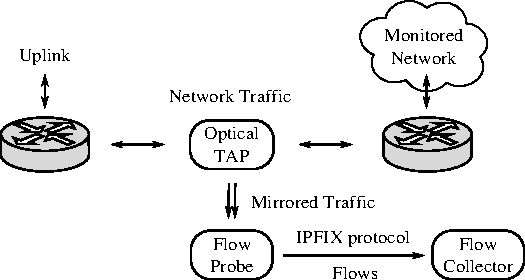
\includegraphics[width=0.8\textwidth]{figures/paper-characterization/monitoring_architecture}
                \caption{Flow Monitoring Architecture Schema} \label{fig:characterization-monitoring-architecture}
        \end{center}
\end{figure}

Flow exporters are configured to create flows with an active timeout of 300 seconds and an inactive timeout of 60 seconds. The flows are terminated using only these timeouts, TCP FIN and RST flags are not used for the flow termination. The exporters use a standard flow key consisting of IP addresses, L4 protocol and its ports. It is important that exporters have the same configuration, since different configurations may result in a different number of exported flow records. As we will show, the number of flow records is an important characteristic of the network.

The flows from all probes are collected on a single collector. No sampling is used in the flow creation or collection process; therefore we have a complete flow trace of the measured network in a given period of time.


\subsubsection{Data Preprocessing}

This subsection describes how the raw flow data was processed. First, we generate statistics for short intervals so that the amount of data is reduced. These statistics do not carry any personal information, therefore they can be shared with other researchers without privacy concerns. Then we process these statistics, look at daily and weekly patterns, their averages and deviations. We identify characteristics which differ between the networks, describe them and use them to differentiate between the networks. To be able to compare the traffic characteristics of different networks, we need to normalise the volumetric properties of the traffic.

Individual flow records are not needed to describe network traffic. Instead, the records must be aggregated and statistical indicators must be derived from the raw data. Since most flow-based frameworks process data in 5 minute intervals~\cite{Haag-2011-NfSen}, we chose the same interval for generating aggregated statistics.

We generate five types of statistics from the original flow records: \emph{Basic volume}, \emph{Advanced volume}, \emph{Layer 3}, \emph{Layer 4} and \emph{Layer 7} statistics. These statistics are listed in Table~\ref{tab:characterization-collected-statistics}. There are 41 collected statistics in total when the bytes, packets and flows statistics are counted separately. 

\begin{table}[!t]
        \centering
        \renewcommand{\arraystretch}{1.1}
        \begin{tabular}{|c|l|} \hline
            \textbf{Type} & \textbf{Statistic} \\ \hline
            \multirow{3}{*}{Basic Volume} & Bytes per second \\
            & Packets per second \\
            & Flows per second \\ \hline
            \multirow{2}{*}{Advanced volume} & Flow size in packets, bytes \\
            & Flow connection length \\ \hline
            \multirow{3}{*}{Layer 3} & Source host count \\
            & Destination host count \\
            & IPv4 / IPv6 bytes, packets, flows \\ \hline
            \multirow{4}{*}{Layer 4} & IPv4 / IPv6 TCP bytes, packets, flows \\
            & IPv4 / IPv6 UDP bytes, packets, flows \\
            & IPv4 / IPv6 ICMP bytes, packets, flows \\
            & IPv4 / IPv6 other protocol bytes, packets, flows \\ \hline
            \multirow{1}{*}{Layer 7} & Top 10 ports by packets, bytes, flows \\
            \hline
        \end{tabular}
        \caption{Collected Statistics}
        \label{tab:characterization-collected-statistics}
\end{table}

The Advanced volume statistics represent the detailed volumetric characteristics of the network. Therefore, we compute mean, variance, standard deviation, median and all percentiles from 0.55 to 0.95 with increment of 0.05. Percentiles lower than the median are superfluous since half of the flows in every network are composed from single packet flows, which amount to zero length flows with small packet sizes (typically 40 bytes). We also computed covariance and correlation for each pair of these statistics. The port statistics are stored as a table of top 10 ports sorted by either packets, bytes or flows. We also the computed overall top port statistic for our analysis.

\subsection{Results} \label{subsec:characterization-results}
We carefully considered all the acquired data and divided it into seven areas of network behaviour that are studied in more detail. This section describes our findings and decisions taken when analysing the collected data.


\subsubsection{Day-night Pattern}

The day-night pattern is a key element of change in every network with human users. It is evident that we cannot compare traffic captured during the day with traffic captured at the night. The reason is that the traffic pattern during the night generally contains much less user generated traffic and the properties are very different, as we present further in our analysis. The day-night pattern is best observed in flows per second since it expresses the number of connections. Using bytes or packets per second distorts the pattern since there are heavier flows during the day than at the night~\cite{Quan-2010-Characteristics}. It is possible to use the number of hosts to show the day-night pattern but the results are very strongly correlated, therefore we decided to use flows per second.

\begin{figure}[!t]
        \begin{center}
                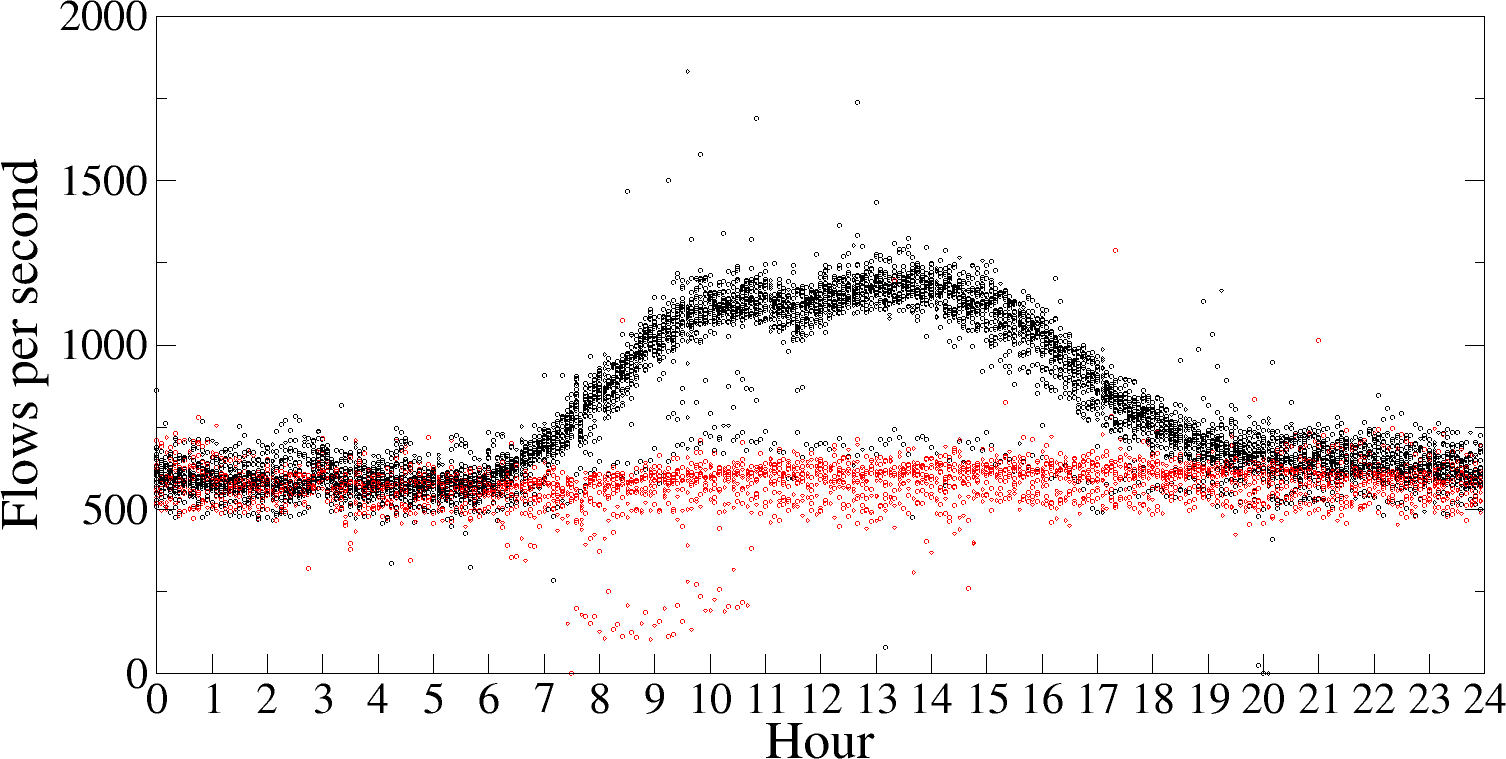
\includegraphics[width=\columnwidth]{figures/paper-characterization/flows-ukb-jan}
                \caption{Flows per Second in the UCB Network} \label{fig:characterization-flows-ukb-jan}
        \end{center}
\end{figure}

The day-night behaviour of the network discloses a lot of information about the purpose of the network. Figure~\ref{fig:characterization-flows-ukb-jan} shows flows per second in University Campus Bohunice network in January. The data from all the days is superimposed in the graph so that the day-night pattern is clearly visible. The red colour shows the weekends and the black is for workdays. It is possible to even see a lunch break in the data at half past eleven. The weekends are flat and do not exhibit the day-night patterns since there are not many users at the weekend.

\begin{figure}[!t]
        \begin{center}
                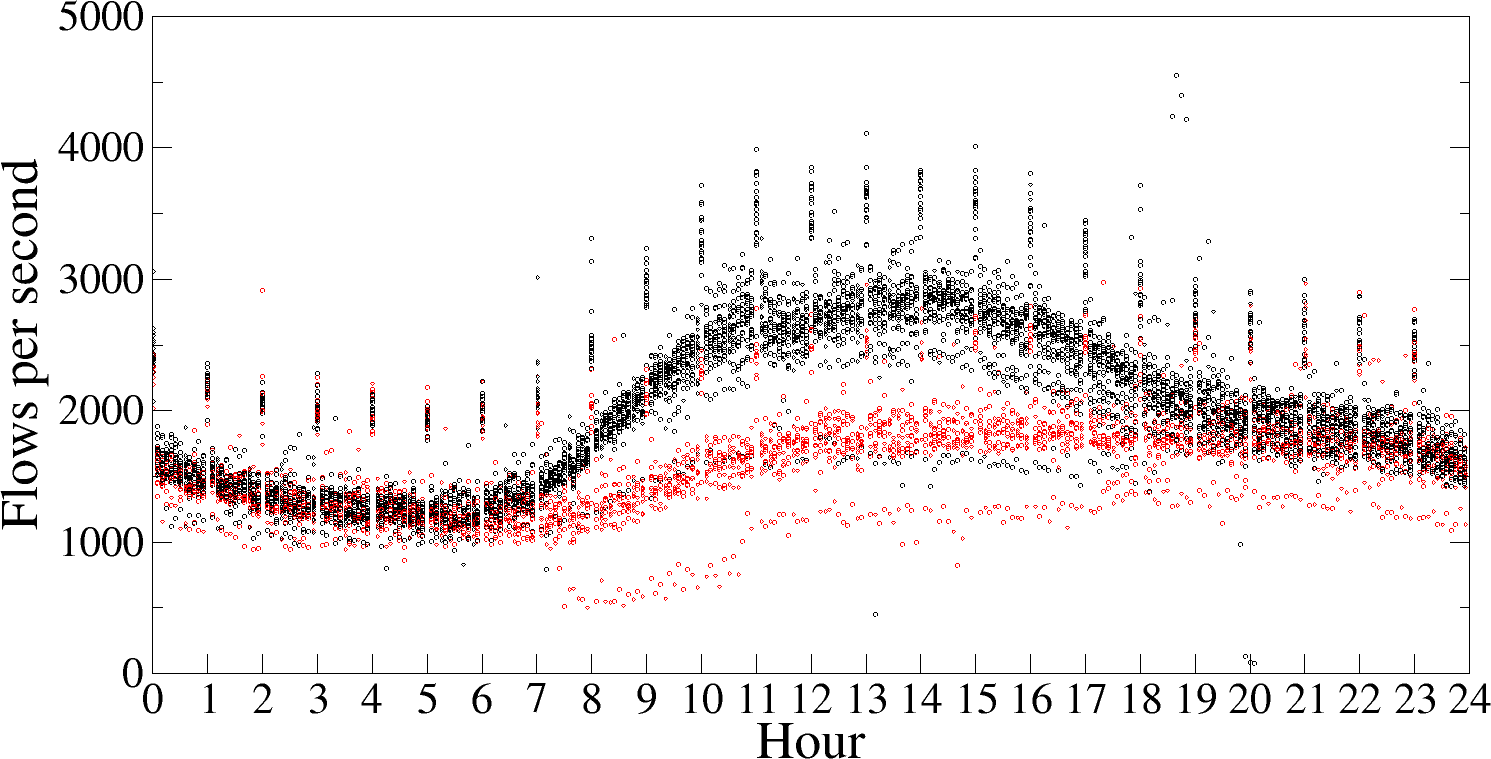
\includegraphics[width=\columnwidth]{figures/paper-characterization/flows-vss-jan}
                \caption{Flows per Second in the VSS Network} \label{fig:characterization-flows-vss-jan}
        \end{center}
\end{figure}

Figure~\ref{fig:characterization-flows-vss-jan} shows the Virtual Switching Segment network which has quite different properties. Since there are Eduroam users and servers that are accessed from outside the university, we can see that there is a day-night pattern visible even at the weekends. Moreover, we can see periodical communication which is caused by automated server backups and updates.

%Darkest night (5) brigtest day (12 ukb, ics,  14 fi, mu, vss) in January, March is different for ics night and fi day
\begin{table}[!htb]
        \centering
        \renewcommand{\arraystretch}{1.1}
        \begin{tabular}{|l|r|r|r|r|r|r|} \hline
                \multirow{2}{*}{\centering\textbf{Network}}  & \multirow{2}{*}{\centering\textbf{Day}} & \multirow{2}{*}{\centering\textbf{Night}} & \multicolumn{2}{c|}{\textbf{Day-night Ratio}}  & \multicolumn{2}{c|}{\textbf{Week Ratio}}  \\ \cline{4-7}
                & & & \textbf{January} & \textbf{March} & \textbf{January} & \textbf{March} \\ \hline
                \textit{UCB} & 13 & 5 &  1.96 & 2.08 & 1.85  & 1.87 \\ \hline
                \textit{ICS} & 13 & 1 & 2.25  & 1.70 & 2.24 & 1.52 \\ \hline
                \textit{MU} & 14 & 5 & 3.08 & 3.62 & 1.45 & 1.95 \\ \hline
                \textit{FI} & 10 & 5 & 2.04 & 2.16 & 1.47 & 1.64 \\ \hline
                \textit{VSS} & 14 & 5 & 2.16 & 2.73 & 1.43 & 1.77 \\ \hline
        \end{tabular}
        \caption{Day to Night and Workday to Weekend Ratio According to Flows per Second}
        \label{tab:characterization-day-night-ratio}
\end{table}

For each network the most and the least busy hour of the day according to flows per second was determined (as shown in Table~\ref{tab:characterization-day-night-ratio}). Given the property of the network, the \textit{day-night ratio} will be, from now on, computed as a ratio between the average of the property during the busiest hour in the day and the least busy hour at night. Using day-night ratios specific to each network allows us to compare the behaviour of each network regardless of the absolute size of the network. 
%Otherwise, we would have to propose a \emph{standard day} and apply a timezone correction before computing the ratios. Unfortunately, we do not have access to a network in different timezone to compare the results and we present all data in the Europe/Prague timezone for simplicity.

Table~\ref{tab:characterization-day-night-ratio} also describes the day-night pattern for all networks. We processed the data from January and March 2015 separately to show the difference between the exam period and the teaching period. The day-night ratio expresses the ratio of flow count as described earlier. The largest difference between the day-night ratios in January and March is in the traffic from the entire university and the VSS traffic. This is a seasonal change caused by students leaving the campus and returning only for their exams. The traffic from faculty networks (FI, VSS) increases only slightly in the teaching period, indicating that the faculty networks are not highly utilised by students. The ICS network shows the opposite trend, which is likely caused by project deadlines and people working harder after the Christmas vacation to meet them.

We also computed an interval which has the maximal ratio of average flows per second to the rest of the day. We have observed two types of network. The activity in networks FI, MU and VSS start at circa 7:00 and ends at 23:00, while the activity in networks UCB and ICS start at 8:00 and ends at circa 17:00. This can be attributed to the fact that that UCB and ICS networks are used while people work and the rest of the networks are used while people are awake.

The day-night pattern provides important information about the networks and their usage. We can use figures from Table~\ref{tab:characterization-day-night-ratio} to describe the day-night pattern of these networks.

\subsubsection{Weekday Pattern}

Another significant pattern that can be observed in network traffic is the weekday pattern. Figures~\ref{fig:characterization-flows-week-ukb-jan} and~\ref{fig:characterization-flows-week-vss-jan} show the weekday pattern in January for UCB and VSS. The graphs are constructed by superimposing the data from individual weeks. There are significant differences between the networks. The weekend traffic at UCB is almost flat but VSS shows behaviour that suggests that there is a significant number of users communicating over the network even at weekends.
%
\begin{figure}[!t]
        \begin{center}
                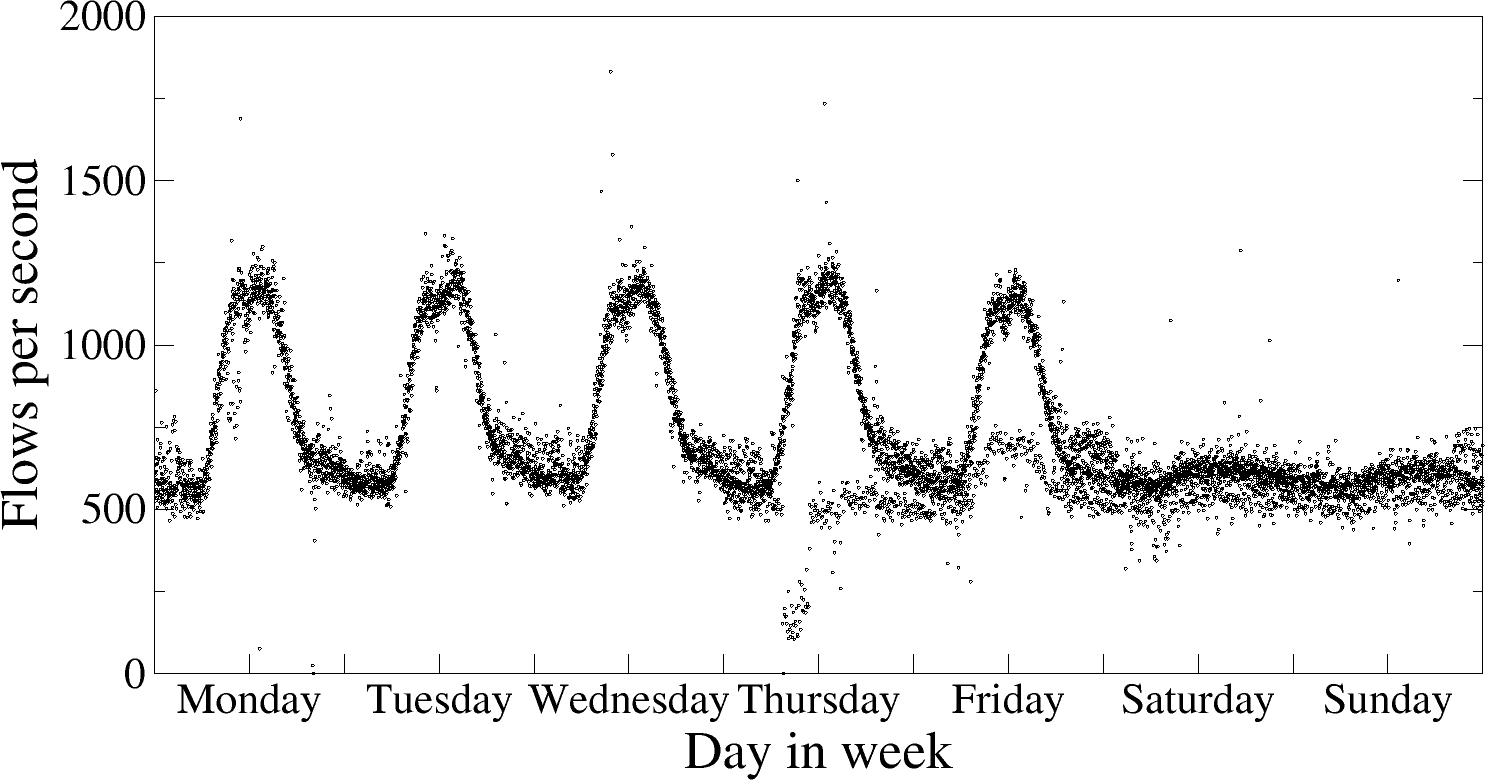
\includegraphics[width=\columnwidth]{figures/paper-characterization/flows-week-ukb-jan}
                \caption{Flows per Second in the UCB Network} \label{fig:characterization-flows-week-ukb-jan}
        \end{center}
\end{figure}

\begin{figure}[!htb]
        \begin{center}
                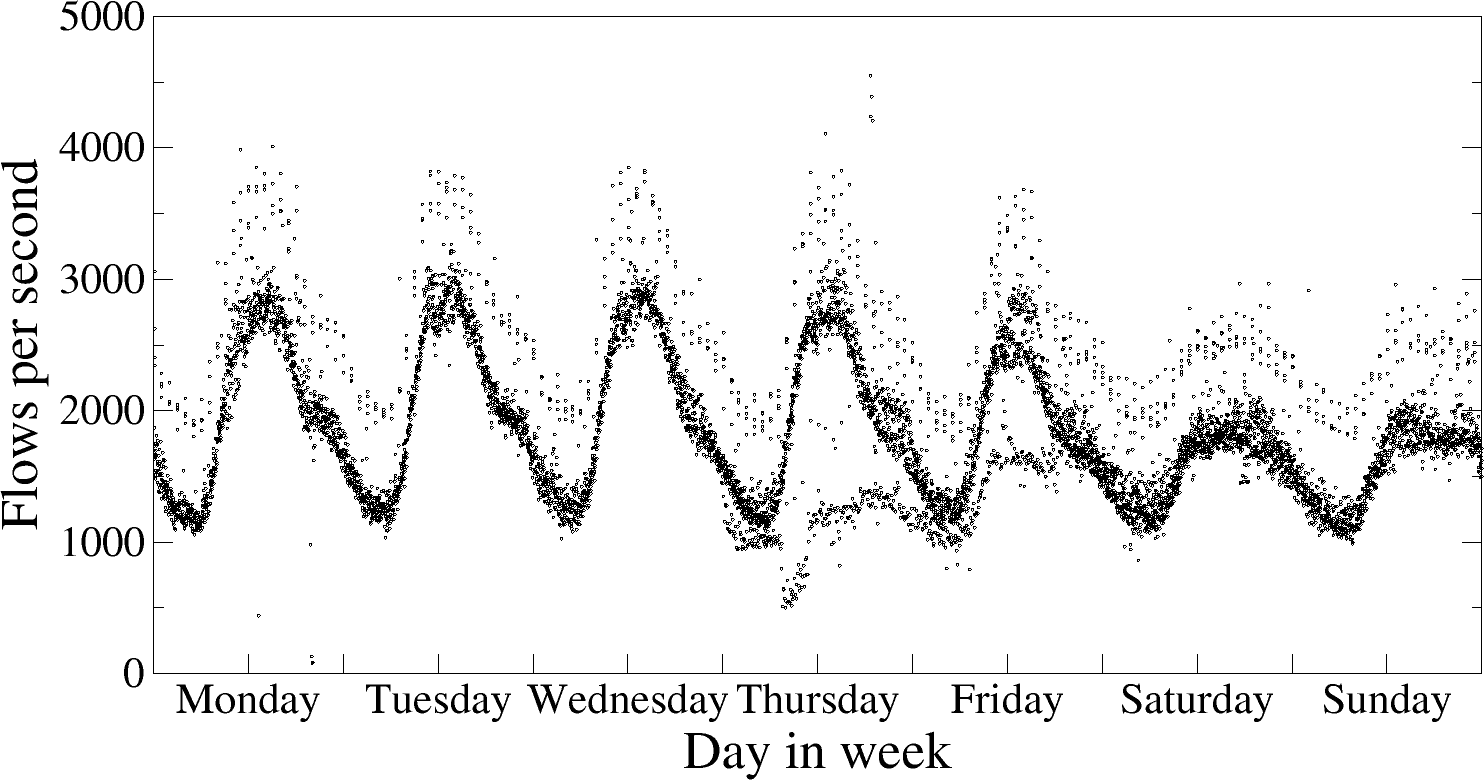
\includegraphics[width=\columnwidth]{figures/paper-characterization/flows-week-vss-jan}
                \caption{Flows per Second in the VSS Network} \label{fig:characterization-flows-week-vss-jan}
        \end{center}
        \vspace{-1mm}
\end{figure}

The difference between work days and weekends can be expressed as a ratio of average flows per second measured during the busiest hours on workdays and at weekends. Table~\ref{tab:characterization-day-night-ratio} shows the results for January and March. This characteristic shows a correlation with the day-night pattern. 
We presume that if the network is accessed by other users, such as students, outside working hours, it will probably be accessed also on weekends by the same users.
% We presume that this is caused by the fact that when the network has other users than employees, such as students, these user will generate network traffic in night hours as well as during the weekends. 
However, we can still employ this statistic to differentiate between networks, since the correlation is not strong and the statistic still adds new information.

\subsubsection{Flow Characteristics}

Using basic network characteristics such as packets per flow, bytes per packet, flow length or number of hosts is difficult due to day-night and weekly patterns. The variance of these variables renders averaging the values useless. Therefore, we have taken another approach. Average values are computed for whole weeks and the averages are used as base values. The variance of week averages computed over the months is on average less than 10\,\%, which is low enough to use these values to characterise the networks. 

\begin{table}[!t]
        \centering
        \renewcommand{\arraystretch}{1.1}
        \setlength{\tabcolsep}{5pt}
        \begin{tabular}{|l|r|r|r|r|} \hline
                \multirow{2}{*}{\centering\textbf{Network}} & \multicolumn{2}{c|}{\textbf{Length of The Flow}} & \multicolumn{2}{c|}{\textbf{Packets per Flow}} \\ \cline{2-5}
                  & \textbf{Week avg.} & \textbf{Day-night rat.} & \textbf{Week avg.} & \textbf{Day-night rat.} \\ \hline
                \textit{UCB} &  10.07 s & 2.18 &  112.86 & 1.28 \\ \hline
                \textit{ICS} & 10.34 s & 1.68 & 205.36 &  0.66 \\  \hline
                \textit{MU} & 13.09 s & 2.13 & 71.79  & 0.81 \\  \hline
                \textit{FI} & 5.40 s & 1.77 & 67.60 & 0.70 \\  \hline
                \textit{VSS} & 7.14 s & 2.04 & 106.25 & 0.94 \\  \hline
        \end{tabular}
        \caption{Average Length of Flow and Packets per Flow}
        \label{tab:characterization-avg-lengths}
\end{table}

Bytes per packet statistic had little variance over the measured networks and it gives almost no information to discern the networks. We found that flow length and packet per flow statistics differ more significantly, as shown in Table~\ref{tab:characterization-avg-lengths}, and can be used to discern the networks. The day-night ratios show that the networks with similar averages might have different day-night behaviour for the same statistics. Therefore, the ratios add new information to the week averages.

\begin{table}[!t]
        \centering
        \renewcommand{\arraystretch}{1.1}
        \begin{tabular}{|l|c|c|c|c|} \hline
                \multirow{2}{*}{\centering\textbf{Network}} & \multicolumn{2}{c|}{\textbf{Source Hosts}} & \multicolumn{2}{c|}{\textbf{Destination Hosts}} \\ \cline{2-5}
                  & \textbf{January} & \textbf{March} & \textbf{January} & \textbf{March} \\ \hline
                
                \textit{UCB} & 2.66 & 2.51 & 1.91 & 1.90 \\ \hline
                \textit{ICS} & 2.76 & 3.11 & 1.99 & 2.35 \\ \hline
                 \textit{MU} & 2.49 & 2.66 & 1.65 & 2.08 \\ \hline
                \textit{FI} & 1.24 & 1.35 & 1.22  & 1.31 \\ \hline
                \textit{VSS} & 2.93 & 4.93 & 2.48 & 4.12 \\ \hline
        \end{tabular}
        \caption{Source and Destination Hosts Day-Night Ratios}
        \label{tab:characterization-day-night-hosts-ratio}
\end{table}

The average number of hosts is a statistic directly related to the size of the network and cannot be used to describe the type of the network without normalisation. Therefore, we use only the day-night host ratios, as shown in Table~\ref{tab:characterization-day-night-hosts-ratio}, which are independent of the absolute number of hosts. Source and destination directions are determined by the direction of the flow. There is a significant difference between host ratios in January and March for the VSS network. The UCB is quite indifferent in comparison, as the ratios remain almost the same. This shows that the statistic can be used to find differences between the networks.

We have shown that comparing basic characteristics on networks must be done in sufficiently large intervals that are the same for all networks. In our case the average values taken over an entire week proved to be stable enough to be used as a network characteristic. The ratio between characteristics measured during the day and night period also provides relevant information about the behaviour of the network and can also be used as an important network characteristic.


\subsubsection{IPv6 Utilisation}

The utilisation of the IPv6 protocol in the network is a Layer 3 characteristic that indicates the technological readiness of the network. The adoption of IPv6 is slow and IPv4 traffic is still dominant. We use this fact to differentiate between networks with different levels of IPv6 readiness. The amount of IPv6 traffic is affected by IPv6 ready servers in the networks and IPv6 services accessed by users outside the network. Table~\ref{tab:characterization-ipv6-utilization} shows the ratio of IPv6 to total traffic in flows, packets and bytes. The packets and bytes ratios are strongly correlated, however, they differ from the flows statistic. The UCB, ICS and MU networks clearly stand out in these characteristics.

\begin{table}[!t]
        \centering
        \renewcommand{\arraystretch}{1.1}
        \begin{tabular}{|l|r|r|r|} \hline
 \textbf{Network} & \textbf{Flows} & \textbf{Packets} & \textbf{Bytes} \\ \hline
 \textit{UCB} & 0.02\,\% & 0.01\,\% & 0.00\,\% \\ \hline
 \textit{ICS} & 5.58\,\% & 12.35\,\% & 13.57\,\% \\ \hline
 \textit{MU} & 12.98\,\% & 1.94\,\% & 1.41\,\% \\ \hline
 \textit{FI} & 3.22\,\% & 2.04\,\% & 2.10\,\% \\ \hline
 \textit{VSS} & 4.66\,\% & 0.23\,\% & 0.17\,\% \\ \hline
        \end{tabular}
        \caption{IPv6 Utilisation}
        \label{tab:characterization-ipv6-utilization}
\end{table}


\subsubsection{Protocol Share}

We investigated the differences in Layer 4 protocol usage in the data sets. TCP and UDP are the dominating protocols in all networks and the shares of ICMP and other protocols are so negligible that they can hardly be used to describe the networks. The shares of TCP and UDP differ significantly between day and night time. Table~\ref{tab:characterization-tcp-udp-share-flows-table} shows the average TCP and UDP shares during the day and night in flows.

\begin{table}[!t]
        \centering
        \renewcommand{\arraystretch}{1.1}
        \begin{tabular}{|l|r|r|r|r|} \hline
                \multirow{2}{*}{\textbf{Network}} & \multicolumn{2}{c|}{\textbf{Day}} & \multicolumn{2}{c|}{\textbf{Night}} \\ \cline{2-5}
                 & \textbf{Tcp} & \textbf{Udp} & \textbf{Tcp} & \textbf{Udp} \\ \hline
                \textit{UCB} & 38.52\,\% & 59.76\,\% & 19.44\,\% & 77.66\,\% \\  \hline
                \textit{ICS} & 41.26\,\% & 56.88\,\% & 28.20\,\% & 68.84\,\%\\  \hline
                \textit{MU} & 55.55\,\% & 43.03\,\% & 42.99\,\% & 54.25\,\% \\  \hline
                \textit{FI} & 49.96\,\% & 49.07\,\% & 25.15\,\% & 73.49\,\% \\  \hline
                \textit{VSS} & 30.67\,\% & 67.76\,\% & 19.30\,\% & 78.00\,\% \\  \hline
        \end{tabular}
        \caption{TCP and UDP Share in Day and Night in Flows}
        \label{tab:characterization-tcp-udp-share-flows-table}
\end{table}

The increase in TCP traffic during the day is caused by users since most of the services use the TCP protocol. We also investigated protocol shares in packets and bytes and found that they match the overall packet to flow and byte per packet ratio. The results show that the TCP to UDP ratio differs between the networks and can be used for their description.

\subsubsection{Most frequent ports}
Traffic analysis by port numbers provides evidence of application usage in the network. Although the port numbers are not considered to be accurate enough for application identification~\cite{Moore-2005-Toward}, most of the traffic adheres to well-known port numbers, which is accurate enough for our purpose. We computed the top 10 port statistics by flows and packets in January and March for all networks. The flows statistic is more stable and more suitable for analysing the behaviour of the network. We selected ten well-known ports that were most often observed in the statistic. Table~\ref{tab:characterization-ports} shows the percentage of flows that belong to these ports. We can observe that the networks have very different usage of the ports which makes port usage an important characteristic of the network. Note that we did not study day-night variance of port usage, but we expect that its fluctuation may be used to refine the results.

\begin{table}[!t]
        \centering
        \renewcommand{\arraystretch}{1.1}
        \begin{tabular}{|c|c|r|r|r|r|r|} \hline
                \multicolumn{2}{|c|}{\textbf{Port / Network}} & \textbf{UCB} & \textbf{ICS} & \textbf{MU} & \textbf{FI} & \textbf{VSS} \\ \hline
                \textbf{DNS} & \textbf{53} & 9.7\,\% & 30.2\,\% & 21.5\,\% & 12.2\,\% & 42.7\,\% \\ \hline
                \multirow{2}{*}{\textbf{HTTP(S)}} & \textbf{80} & 9.2\,\% & 7.4\,\% & 20.2\,\% & 16.8\,\% & 5.9\,\% \\ \cline{2-7}
                & \textbf{443} & 6.5\,\% & 8.3\,\% & 14.7\,\% & 20.1\,\% & 4.0\,\% \\ \hline
                \multirow{2}{*}{\textbf{Mail}} & \textbf{25} & -- & -- & 1.0\,\% & 0.6\,\% & -- \\  \cline{2-7}
                & \textbf{993} & -- & 1.7\,\% & -- & 0.6\,\% & -- \\ \cline{1-7}
                \textbf{Samba} & \textbf{445} & 1.0\,\% & -- & -- & -- & 0.7\,\%  \\ \hline
                \textbf{SSH} & \textbf{22} & -- & -- & 1.4\,\% & 0.3\,\% & -- \\ \hline
                \textbf{NTP} & \textbf{123} & -- & 0.9\,\% & 7.1\,\% & 43.9\,\% & -- \\ \hline
                \textbf{SNMP} & \textbf{161} & 52.8\,\% & 11.9\,\% & -- & -- & 23.5\,\% \\ \hline
                \textbf{Telnet} & \textbf{23} & 1.0\,\% & 1.3\,\% & 1.6\,\% & 0.4\,\% & -- \\ \hline
        \end{tabular}
        \caption{The Most Common Ports by Flows in January}
        \label{tab:characterization-ports}
\end{table}

\subsection{Conclusions} \label{subsec:characterization-conclusions}

We have presented an analysis of network traffic measured at five different campus networks at Masaryk University. Our goal was to show that the properties of the networks can be extracted and quantified and that we can use the results to differentiate and describe the networks. We have made several observations during our analysis which affect the derivation of network characteristics.

\begin{itemize}
    \setlength\itemsep{4pt}
    \item Flow-based statistics are more stable than byte or packet based statistics. Therefore it is more practical to use flow statistics to track long-term changes in network behaviour.
    \item Day-night and weekday patterns must be taken into consideration when computing network characteristics.
    \item Long enough samples of the traffic must be available.
    \item Using ratios between day and night helps to compensate for the day-night pattern and the size of the network. However, there is still a slight correlation between network size and the day-night ratios.
    \item To describe a network used to perform an experiment, the description of behaviour using network characteristics should be complemented with absolute volumetric information.
\end{itemize}

Our measurements have confirmed that it is possible to differentiate between networks based on the observed characteristics. Moreover, the campus networks showed quite stable characteristics over time even though the measurements were taken during the winter exam and spring teaching periods. Furthermore, we tested the correlation of the described characteristics and found that they are only very weakly correlated. This shows that each of the characteristics is valuable and carries information about the network. However, the presented characteristics are not by any means complete. We analysed a subset of possible characteristics derived from flow records, which can be easily measured on a network. Thus we believe that more work is required to identify other useful characteristics and utilise them to describe the behaviour of the networks.


\section{Summary}\label{sec:use-cases-summary}

% HTTP security monitoring
In the first section, we presented an analysis of HTTP traffic in a large-scale environment which uses application flow monitoring with HTTP protocol processing. In contrast to previously published analyses, we were the first to classify patterns of HTTP traffic which are relevant to network security. We described three classes of HTTP traffic which contain brute-force password attacks, connections to proxies, HTTP scanners, and web crawlers. Using the classification, we were able to detect up to 16 previously undetectable brute-force password attacks and 19 HTTP scans per day in our campus network. The activity of proxy servers and web crawlers was also observed. Symptoms of these attacks may be detected by other methods based on basic flow monitoring, but detection using the analysis of HTTP requests is more straightforward. We, thus, confirm the added value of application flow monitoring in comparison to the traditional method.

% IPv6 tunnels
The exhaustion of IPv4 address space increases pressure on network operators and content providers to continue the transition to IPv6. The IPv6 transition mechanisms such as Teredo and 6to4 allow IPv4 hosts to connect to IPv6 hosts. On the other hand, they increase network complexity and render ineffective many methods to observe IP traffic. In Section~\ref{sec:analysis-ipv6-transition}, we extended our flow-based measurement system to involve transition mechanisms information to provide full IPv6 visibility. Our traffic analysis focuses on IPv6 tunneled traffic and uses data collected over one week in the Czech national research and education network. The results expose various traffic characteristics of native and tunneled IPv6 traffic, among others the TTL and HOP limit distribution, geolocation aspect of the traffic, and list of Teredo servers used in the network. Furthermore, we show how the traffic of IPv6 transition mechanisms has evolved between 2010 and 2013.

% Geolocation
The importance of IP address geolocation has increased significantly in recent years, due to its applications in business advertisements and security analysis, among others. Current approaches perform geolocation mostly on-demand and in a small-scale fashion. As soon as geolocation needs to be performed in real-time and in high-speed and large-scale networks, these approaches are not scalable anymore. To solve this problem, we propose two approaches to large-scale geolocation in Section~\ref{sec:analysis-geolocation}. Firstly, we present an exporter-based approach, which adds geolocation data to flow records in a way that is transparent to any flow collector. Secondly, we present a flow collector-based approach, which adds native geolocation to NetFlow data from any flow exporter. After presenting prototypes for both approaches, we demonstrate the applicability of large-scale geolocation by means of use cases. Our prototypes have shown to be scalable enough for deployment on the 10\,Gbps Internet connection of the Masaryk University.

% Traffic characterization
Performing research on live network traffic requires the traffic to be well documented and described. The results of such research are heavily dependent on the particular network. Section~\ref{sec:analysis-characterisation} presents a study of network characteristics, which can be used to describe the behaviour of a network. We propose a number of characteristics that can be collected from the networks and evaluate them on five different networks of Masaryk University. The proposed characteristics cover IP, transport and application layers of the network traffic. Moreover, they reflect strong day-night and weekday patterns that are present in most of the networks. Variation in the characteristics between the networks indicates that they can be used for the description and differentiation of the networks. Furthermore, a weak correlation between the chosen characteristics implies their independence and contribution to network description.
